\documentclass[english]{yMasterThesis}

\usepackage[
  backend=biber,
]{biblatex}
\addbibresource{2022-06-15_master_thesis.bib}

\title{GitDAO, Blockchain Primitives for Open Source}
\author{Harvey Sheppard}

\makeatletter%
\hypersetup{%
  pdfauthor=\@author,
  pdftitle=\@title,
  pdfkeywords={Governance, Open source, Blockchain, DAO, Decentralization},
  pdfsubject={Building blockchain-based primitives to improve collaboration in the open source ecosystem.},
}%
\makeatother%

% \includeonly{tex/titlepage}

\begin{document}

\begin{titlepage}
  \symmetricalPage%
  \begingroup%
    \tikzset{external/export=false}%%
    \begin{tikzpicture}[
        overlay,
        remember picture,
      ]
      \node[anchor=center] at (current page) {\printImageToMinArea{\paperwidth}{\paperheight}{images/sectioning/titlepage/1/img.jpg}};
    \end{tikzpicture}
  \endgroup%
  \sffamily%

  \vspace*{2cm}%
  \begingroup%
    \bfseries%
    % \scshape%
    \begingroup%
      \Huge%
      \color{gray_30}
      GitDAO\\[8mm]
    \endgroup%
    \begingroup%
      \huge%
      \color{gray_30}%
      Blockchain Primitives\\[2mm]
      for Trustless Open Source%
    \endgroup%
  \endgroup%

  \vfill%
  \parbox[b]{\linewidth-6cm}{%
    \begingroup%
      \bfseries%
      \color{gray_90}%
      A Master Thesis.

      \vspace*{7mm}%
      Supervised by\\
      Yann \textsc{Vonlanthen}, Robert \textsc{Ott},\\
      and Prof. Dr. Roger \textsc{Wattenhofer}.
    \endgroup%
  }%
  \hfill%
  \parbox[b]{4cm}{%
    \includesvg[width=\linewidth]{images/sectioning/titlepage/eth_logo_kurz_neg.svg}
  }
\end{titlepage}
\restoregeometry%

\pageBackground%
\marginElement{
$\uparrow$ Photo by \href{https://unsplash.com/@dearjamie?utm_source=unsplash&utm_medium=referral&utm_content=creditCopyText}{Jamie Hagan} on \href{https://unsplash.com/}{Unsplash}.
}
Realized between March and September 2022.

\null\vfill

\begingroup%
% \begin{fullwidth}
  \yTitleContrasted{Abstract}
  \renewcommand{\strong}[1]{{\bfseries\textcolor{gray_20}{#1}}}

  Open source software has become a crucial infrastructure in contemporary societies which is why it is important to protect it.
  This work aims to design blockchain primitives that make open source \strong{trustless}.
  We explore a key element of trustlessness: \strong{decentralization}; why we care about it, and how to achieve it.
  The main proposal of this work is a voting system based on \strong{tokens with time-decreasing power}, which opens a new design space for voting systems, including creating incentives for recurrent contributions and lowering power entrenchment.
  Additionally, we propose a \strong{rewarding scheme} to define the power of the tokens that should be awarded for contributions to an open source project, as well as a \strong{strategy to distribute the money} received by the project to its contributors using the same tokens, aligning value creation and value extraction.
  We propose a \strong{voting workflow} specifically targeted at merge requests that improves security, by providing a challenge mechanism that deters adversarial proposals.
  Finally, we propose a scheme to \strong{back issues} with money for improved community feedback.
  All these features build a coherent specification, called \strong{GitDAO}, that improves the guarantees provided by any open source project that uses it.
% \end{fullwidth}
\endgroup%

\vfill%

\forcedMarginElement{
\includegraphics[width=\linewidth]{images/sectioning/titlepage/switch_logo.png}}%
In collaboration with SWITCH.

\vspace*{1cm}
\forcedMarginElement{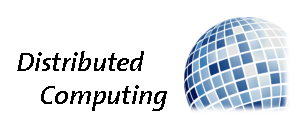
\includegraphics[width=\linewidth]{images/sectioning/titlepage/disco_logo.eps}}%
Done at the Distributed Computing Group,\\[2pt]
Computer Engineering and Networks Laboratory,\\[2pt]
ETH Zürich



\printtableofcontents

\justifying%
\setlength{\parindent}{0ex}

% https://tex.stackexchange.com/questions/51263/what-are-penalties-and-which-ones-are-defined
\clubpenalties=3 1000 500 0 % extra penalty for breaking after first line of a paragraph.
\widowpenalties=3 1000 500 0 % extra penalty for breaking before last line of a paragraph

% \tolerance sets the maximum "badness" that tex is allowed to use while setting the paragraph, that is it inserts breakpoints allowing white space to stretch and penalties to be taken, so long as the badness keeps below this threshold. If it can not do that then you get overfull boxes. So different values produce different typeset result.
% \tolerance 1000

% \emergencystretch (added at TeX3) is used if TeX can not set the paragraph below the \tolerance badness, but rather than make overfull boxes it tries an extra pass "pretending" that every line has an additional \emergencystretch of stretchable glue, this allows the overall badness to be kept below 1000 and stops TeX "giving up" and putting all stretch into one line. So \emergencystretch does not change the setting of "good" paragraphs, it only changes the setting of paragraphs that would have produced over-full boxes. Note that you get warnings about the real badness calculation from TeX even though it retries with \emergencystretch the extra stretch is used to control the typesetting but it is not considered as good for the purposes of logging.
% \emergencystretch 4em
\sloppy

\nomargintoc%
\nomarginimagecaption%
\chapter{Introduction}
\label{sec:introduction}

\leavevmode\marginElement{The \enquote{Affaire Maudet}}%
\marginElement{\input{images/sectioning/horizontal/\arabic{image_sectioning_horizontal}/readme.tex}}%
August 30\textsuperscript{th}, 2018, Geneva, Switzerland, the public ministry announces that it wants to investigate an elected official of the executive branch for illegally accepting benefits from a sheik in Abu Dhabi.
This is only the opening of the so-called \enquote{Affaire Maudet}, which will see many developments, and still be instructed at the federal level four years later.
In the face of public criticism and pressure, the magistrate refuses to resign, even after multiple bodies such as the executive chamber of the government and his party ask for his resignation letter.
There is no legal basis to revoke an elected official during its mandate, and so the magistrate will keep his position for two more years.
During this time, the other members of the executive create a new department with almost no influence over the conduct of the state, specifically for the suspected official.
The department he was previously assigned to, the police and justice department, is reassigned to the other magistrates thus impeding the smooth working of the body.
A law making it possible to revoke a magistrate is proposed and accepted by the people of Geneva during the November 21\textsuperscript{st}, 2021 votation.

\leavevmode\marginElement{The Yellow Vests}Winter 2018, the French yellow vests, a movement composed mostly of the lower classes, manifests every Saturday against their government by blocking roads.
They want the new proposed tax on fuel dropped, ask for more transparency from the state, more accountability, and the instauration of the citizens' initiative referendum among other revendications.
The protest makes the divide and lack of trust between the people and the French government explicit.
The movement sparks violent demonstrations; the Champs-Élysées and the Arc de Triomphe are ransacked on December 1\textsuperscript{st}, 2018.

\leavevmode\marginElement{Attack on the Capitol}January 6\textsuperscript{th}, 2021, supporters of Donald Trump attack the capitol in Washington, D.~C. after repeated allegations by the former president that the election has been \enquote{stolen} by the Democrats.
Trust in an established institution like the American voting process eroded at a speed that surprised many.

\leavevmode\marginElement{\textit{Roe v. Wade}}June 24\textsuperscript{th}, 2022, the supreme court overturns \textit{Roe v. Wade}, and so suppresses the federal right to abortion in the United States of America.
The decision has since been dubbed \enquote{one of the most undemocratic decisions} of the court, as 61\% of the American people think that it should have remained part of the law \cite{smith_mockery_2022}.

\leavevmode\marginElement{Democratic Issues}Many well-established democracies seem to be facing democratic crises.
Most governments that exist today were created centuries ago, at times during which the technological limitations were more drastic than today.
The ensuing systems had to be designed around those limitations, and therefore provide fewer guarantees than what might be possible and expected today.

\leavevmode\marginElement{The Open Source}When exploring new frontiers of governance systems, the open source ecosystem is inspirational material, as it has been at the forefront of technology, and thus explored new ways to coordinate enabled by modern means.
One of the key properties of open source is the ability to \textit{fork} a project.
Forking is the process of branching off from a project to start your own using the same starting code.
Many projects try to avoid forks as they split the community and the developer time each project receives.
Coordination is generally a better survival strategy in the open source.
This creates incentives for communities to have a governance process satisfying enough.
Note that it is much easier to fork an open source project than to ignite a revolution and bootstrap a new state.
As such, governance systems need to be more optimal in the open source, and when they are not, experiences are conducted at a much faster rate; projects fork, try, rise, and fall over a few months, not a few centuries.
Additionally, there are many more open source projects than there are states, and so the combination of plurality, and fast evolution in this ecosystem implies that it was subjected to a much more strenuous Darwinian selection.

\leavevmode\marginElement{The Blockchain}Blockchain is another domain worthy of attention when it comes to governance systems.
Because blockchains are well suited to transferring value, they enabled a new generation of governance systems that used this primitive to align individual incentives with the greater good more efficiently, than what could be achieved in the open source.
Coordination systems on the blockchain have experimented with various forms and colors, using fungible and non-fungible tokens, having explicit voting procedures or not, and featuring various token distribution mechanisms.
They have been applied to various goals ranging from coordinating a newsletter (BanklessDAO), to managing communities planting trees in Brazil (Toucan Protocol), to deciding the value of obscure protocol parameters of decentralized exchanges (MakerDAO).

\leavevmode\marginElement{Blockchain Speed}Because funds have been injected so quickly into the blockchain ecosystem, hitting an all-time high total value locked of more than 240 billion dollars in December 2021 \cite{noauthor_defillama_nodate}, the ecosystem evolved at an unrivaled speed.
Take for example the \textit{loot} project, an NFT collection of text strings describing adventure game gears, e.g. \emph{Bone Wand} or \emph{Pain Glow Scimitar of Brilliance}.
Brainstormed over a weekend, launched with a single tweet, after a week, the loot NFTs were traded at a staggering minimum value of 15 ETH (\$59'600)...
On the blockchain, the unit to measure the evolution of projects is the week, sometimes it's days.

\leavevmode\marginElement{Blockchain Narratives}The narratives related to blockchain are another reason it is a worthy experimentation ground.
In November 2018, the blockchain was invented by the cypherpunk movement, which notoriously distrusts everybody, especially nation states and banks.
To make a monetary system work without a trusted third party, they came up with various game theoretical mechanisms that make it possible to trust the correctness of a ledger without having to trust any single entity: the blockchain.
This defined the core values of the movement: \emph{decentralization}, \emph{trustlessness}, and \emph{permissionlessness} which all have wide-reaching consequences when applied in the context of governance.
Trustlessness: the system will work as intended without having to trust anyone.
Remember the attack on the American Capitol and the \enquote{stolen} election?
Decentralization and permissionlessness: distribute power in a more egalitarian fashion, and avoid having a minority holding all the power.
Remember \emph{Roe v. Wade}, remember the yellow vests?
Transparency; when everything is open, cheating becomes much harder.
Remember the \enquote{Affaire Maudet}?

\leavevmode\marginElement{Improve Governance of Open Source using Blockchain}We propose in this work to take a new look at governance systems, and what they can bring to open source projects.
How can we use blockchain functionalities to create provably net positive primitives to coordinate open source?
Is it possible to get feedback from users or the community?
Can we ensure that the governance system is inclusive for new contributors?
Can we guarantee that the outcome of the system maximizes the benefit of the entire community, not just a few members?
This work will investigate the use of \emph{decreasing value tokens}, and the limits imposed by the required \emph{sybil resistance}.

\leavevmode\marginElement{Improve Open Source Security}Blockchain can unlock new possibilities in other domains as well.
Take security; a single piece of software generally relies on dozens of libraries.
This creates the software supply chain, and it has been hacked: instead of attacking a well-watched program, corrupt its undefended dependencies.
Some of the most notorious hacks targeted a very simple Javascript library that was left abandoned, but which was used by many blockchain wallets \cite{noauthor_how_nodate}.
Can we provide mechanisms to improve security, like better code reviews or stronger guarantees that useful projects\\are not abandoned?
This work proposes a \emph{voting workflow}, that penalizes adversarial actors.

\leavevmode\marginElement{Improve Monetary Incentives for Open Source}Today, some open source software is embedded in every digital component that exists.
Open source creates priceless value for humanity.
Yet there are almost no developers in the open source ecosystem that are paid for the work they do or the value they create.
This lack of alignment between value creation and value extraction dissuades people from contributing, this is a coordination issue.
Can a blockchain-based system provide means to compensate developers?
This work proposes a \emph{rewarding scheme} and a \emph{monetary distribution mechanism} that incentivizes people to contribute to open source and realigns value creation and value extraction.

\leavevmode\marginElement{Structure of this Work.}
In this work, we will first analyze governance systems, the open source, and blockchain movements to understand them better.
Then, we will propose some blockchain primitives, what we call a \emph{GitDAO}, to improve various aspects of open source and make it more trustless.
Finally, we discuss our attempts at implementing GitDAO.



\part{Theoretical Discussion}

\partSecondPage%
We begin this work with some discussions about governance systems, open source, and blockchain-related topics, as inspiration and guiding lines to create new governance systems for open source projects.
Why these three topics?

Governance systems are the building block required to make decisions and coordinate members of an open source project.
Yet coordination is hard.
Can we create truly decentralized systems?
Does a system exists, that ensures decisions are always satisfying for the participants?
Are there systems that impose little additional friction on users?

Because we are targeting open source projects, exploring their specifics enables us to build systems that are well suited to them.
Some specificities of open source can be exploited; for example, the fact that code is processed through merge requests enables us to limit governance systems to binary decisions.

Finally, we will turn our attention to the blockchain, how it works, what its associated narratives are, how those integrate within the open source philosophy, and what functionalities blockchains can bring to the open source.

\chapter{Governance Systems}
\label{sec:theoretical_governance_system}

\section{Definitions}

We start with a few useful definitions and notations.

\begin{definition}[Decision]
  A decision is an event that must have an outcome fixed by a voting system.
  Decisions are indexed by a counter $i$.
\end{definition}

\begin{definition}[Possible Outcomes]
  The set of possible outcomes for a given decision $i$ is denoted $O_i$.
\end{definition}

\begin{definition}[Users]
  The set of users is denoted $U$.
\end{definition}

\begin{definition}[Votes]
  Let $\Theta_u(i)$ be the vote of user $u$ on decision $i$.
  This is expressed as the preferences of user $u$ over the possible outcomes $O_i$ of decision $i$.
  How preferences are expressed is defined per type of governance system.
\end{definition}

\begin{definition}[Power]
  Let $p_u(t)$ be the absolute power that user $u$ has over the governance system at time $t$, expressed as a floating point number.
\end{definition}

We now define a voting system.

\subsection{Voting Systems}

\begin{definition}[Voting System]
  \label{def:voting_system}
  A voting system is a function $F(\Theta, p, i)$.
  It is applied to the preferences of the users of the system, the power that each user has on the system, and the decision for which to produce an outcome.
  The function returns one outcome from the set of possible outcomes $O_i$.
\end{definition}

Little is specified about how participants should specify their preferences $\Theta$ over the outcomes, and this can be done in different ways: through an ordering (\textit{ranked voting systems}%
\marginNote{%
  In a ranked voting system with three options, a participant might provide the preference $A > C > B$.
}), by assigning some score to each outcome(\textit{cardinal voting system}%
\marginNote{%
  In a cardinal system with three options and where scores are in the range $[-1, 1]$, given that you hate both options $A$ and $B$, but are very much in favor of option $C$, you could submit a preference similar to $\lbrace A: -0.98, B: -0.97, C: 0.85\rbrace$.
}), by distributing a set amount of points among the outcomes, etc.

The power of each user is an important metric.
The power distribution $p$ is defined in absolute terms, yet what interests us is the power that each user has normalized to one, i.e.\ its relative power over the system.

\begin{definition}[Relative Power]
  The relative power of a user $u$ of a voting system on this system at time $t$, denoted $q_u(t)$, is the amount of influence that a particular member can have on an outcome of the system at time $t$ compared to the power of the others, normalized to $1$.
  Mathematically speaking, the relative power is defined as:

  \begin{equation}
    \label{eqn:relative_power}
    q_u(t) = \frac{p_u(t)}{\sum_{v\in U}p_v(t)}
  \end{equation}
\end{definition}

And it holds that $\forall t,\sum_{u\in U} q_u(t) = 1$.

In essence, someone with relative power $1$ has full power over the system, having relative power $0$ means you have no power, and having power $\sfrac{1}{n}$ means that the power is distributed equally among all members.

The definition above can be applied to many real-life examples.
\textit{Binary voting systems} impose $\forall i, |O_i| = 2$.
In most democracies today $\forall u\forall t, p_u(t) = 1$.
In essence, all users have the same, time-independent power over the outcomes of the decision function.
A dictatorship is a voting system in which one user, the dictator, has a power equal to $1$ and all others have a power equal to $0$.
When considering DAOs and token-based voting, evaluating $p_u(t)$ amounts to counting the amount of \textsc{erc20} tokens owned by each participant (or sum the power of the \textsc{erc721} token owned).
Let us denote the set of token owned by user $u$ at time $t$ as $T_u(t)$.
In \textsc{erc20} token-based voting systems, the power of each participant is equal to the number of \textsc{erc20} token owned by the user: $p_u(t) := |T_u(t)|$.
In \textsc{erc721} token-based voting, the \textsc{erc721} token will generally provide a way to evaluate the power that a given token provides.
For example, each token might have a property called \texttt{power}\\in which case:

\begin{equation}
  \label{eqn:power_in_token_based_voting_systems}
  p_u(t) := \sum_{\tau\in T_u(t)}\tau\mathtt{.power}
\end{equation}

These examples highlight the versatility of the definition of a voting system.

Yet, does this definition encompasses governance systems that we know like states?
How can we formalize indirect democracy, also called representative democracy, which can be seen as a two-stage voting process?
What about specifying how the executive and legislative branches work?
Can we describe referendums with the above definition of a voting system?
No.
A voting system only applies once there is a clear decision to make, a fixed set of outcomes, a fixed set of users, a defined way to express preferences, and a fixed power distribution.
Coming up with a good voting system, e.g.\ one that takes into account the preferences of the users, is already a hard problem (see \cref{sec:arrow_impossibility_theorem}).
But a good voting system is not enough.
Take for example the presidential elections in the United States, even if we assume that the voting process of the Electoral College is perfect, gerrymandering makes it possible to end up with Electoral Colleges that do not represent the opinion of the population, and thus to elect a president that lost the popular vote%
\marginNote{This happened five times in history \cite{noauthor_list_2022}.}.
We need to consider more aspects, so we define a broader concept: \emph{governance processes}.

\subsection{Governance Systems}

\begin{definition}[Governance System]
  \label{def:governance_systems}
  We define a governance system to be any system that uses at least one voting system as a subroutine.
\end{definition}

Note that the outcomes of a governance system might be plural and take many forms, from laws to executive decisions, to judiciary decisions.
Also, the voting system used for each of these domains can vary a lot.

Many systems of interest are \emph{governance systems}, not \emph{voting systems}; a human government is a governance system for example.
Defining the power that a user has over a governance system can be a complex, or even intractable, task.
Take a direct democracy for example.
In such a system, a user, i.e.\ a citizen, will have a power equal to that of every other citizen to decide the laws of the country, but how do we account for the executive and judiciary decisions made using some other systems?
In an \emph{indirect} democracy, what is the power that a user has over laws?
More complex even, consider the Swiss governance system and the ability to start referendums on laws voted by Parlament: once a law is voted by our representatives, a subset of the population can come together to challenge the law.
Not being able to evaluate the power of a user over a governance system is an issue, especially when we try to formalize what democracies are.
Do you remember the \enquote{most undemocratic decision} taken by the American supreme court when it overturned \textit{Roe v. Wade}?
What does it mean to be undemocratic in this case?
Most blockchain-based systems are much simpler, because their scope is a lot more limited, and so they are easier to analyze.
Happily enough, this work focuses on creating a blockchain system.

Let's consider for a brief moment what we mean by democracies.
What does it mean to give power to the people?
Most people define a democratic system as a majority system, where the majority opinion is computed using the same weight for each citizen.
This explains well the \enquote{undemocratic} aspect of \textit{Roe v. Wade}.
But how does this definition integrate with the rule of law?
Laws evolve rather slowly; can a law \emph{become} undemocratic if citizen change their mind about a topic?
And what about giving a lot more power to some individuals that can use it to influence the system without having strong accountability (think \enquote{Affaire Maudet}, the executive branch and the legal immunity that it grants, or any judge in the legal system)?
Are those undemocratic ways of conducting a state?
Is democracy the ultimate goal?
We leave it Open to find a more satisfying definition of \emph{democratic}, and to define then whether it is a goal worth pursuing.

\section{Properties}

In the next sections, we look at desirable properties, or on the contrary, that we would like to avoid for voting systems and governance systems.

\subsection{ Arrow's Impossibility Theorem}
\label{sec:arrow_impossibility_theorem}

Let's first come back to voting systems.
Many functions fulfill the requirements of \cref{def:voting_system}.
For example, the function that always returns the first outcome in $O$ is a valid voting system that does not take user preferences into account.
Of course, this is not so interesting, so we define a few additional properties that we want our voting system to fulfill.

\begin{property}[Pareto Efficiency]
  \label{prop:pareto_efficiency}
  If every participant prefers option $A$ over option $B$, then the system should prefer option $A$ to option $B$.
\end{property}

\begin{property}[Nondictatorship]
  \label{prop:non_dictatorship}
  The system must take the preferences of multiple participants into account.
  It cannot mimic the preferences of a single user, called the dictator.
\end{property}

\begin{property}[Independence of Irrelevant Alternatives]
  \label{prop:independence_irrelevant_alternatives}
  Adding irrelevant outcomes to a decision, i.e.\ outcomes that no one like, should not change the outcome of the system.
\end{property}

All the properties above seem rather reasonable to expect.
Unfortunately, Arrow's Impossibility Theorem \cite{noauthor_arrows_2022} proves that there exists no ranked voting system that can fulfill all three when there are more than two options to vote on.
So coming up with good voting systems, we are \emph{not} even talking about governance systems, might be harder than expected.

\subsection{Tyranny of the Majority}
\label{sec:tyranny_of_the_majority}

This is a problem that any majority voting system has.
By performing majority votes, up to 50\% of the participants may be left unsatisfied.
If there are 50\% of people that always agree, then the remainder of the population can end up being tyrannized, and live under a set of rules it disagrees with.

In the specific case of binary votes, i.e.\ votes in which there are only two possible outcomes, which do not suffer from Arrow's impossibility theorem, you can require different thresholds to accept a proposal while preserving nondictatorship, Pareto efficiency, and independence of irrelevant alternative.
For example, you can request that at least 60\%\\of votes are in favor to accept a proposal.
Any percentage preserves the three properties above.
Which should we use?
We now show that any percentage different than 50\% can potentially lead to a situation with even more unsatisfied people.
If you use a 60\% threshold---or, by symmetry, a 40\% threshold---, then you can have up to 60\% of people that are dissatisfied with the vote outcome.
Plus, the formulation of the question, i.e.\ \enquote{Are you in favor of adopting law $x$?} or \enquote{Are you in favor of \emph{not} adopting law $x$?}, now has an impact on the outcome.
Who decides how questions are formulated?
Those will have more power than the others.
So the 50\% threshold is the one that maximizes the guaranteed number of satisfied people and avoids introducing more unfairness in the system.

But having potentially 50\% of totally unsatisfied people is a bad situation to be in.
Can we do better?
Maybe voting systems are not well suited to coordinate humans?
Can we find an alternative system that has better properties?
To find an answer to this question we propose to explore a few existing systems in sections \cref{sec:consensus} and \ref{sec:bicameral_systems}.

\subsection{Making Informed Decisions}
\label{sec:making_informed_decisions}

How can we make sure that people vote based on informed, rational judgments and not just some biased preconceptions?
This is of value if we want the outcomes of the governance system to lead its users to an optimal situation.
To distinguish between a good and a bad decision, people need at least to be knowledgeable about the topic they are voting on.
One will generally need to invest time and effort into a topic to become knowledgeable about it.

If votes are held frequently, then it is probably not realistic to expect everyone to invest the time and energy necessary to become knowledgeable about the topics voted on.
This is a problem well known in Switzerland, where votations are held approximately four times a year and where topics can be varied.
So people often resort to not voting at all, or voting along the lines of a party they feel close to.

Are there alternatives to ensuring that the voting users are well informed about the topic?
Here are a few proposals:

\begin{description}
  \item[Expert Groups]
    Each participant is assigned to one or multiple topical groups based on their competencies.
    When a decision is required, a first vote about which expert group should decide for the matter at hand is held, then the selected expert group vote on the question.
    
    Getting this approach right is hard as the process can be attacked in various ways.
    For example, you can vote to assign questions to expert groups that you expect to be of your opinion, or you can join expert groups that get assigned to questions you have opinions about, even if you are not an expert.
    Further, this approach mostly makes sense when there is an unambiguous answer to a technical question for which experts are best suited to answer.
    But there are questions to which there are no optimal answers, either because a lack of data makes it impossible to know \textit{a priori} what the best outcome is, or because it is fundamentally a question of values.
  \item[Liquid Democracies]
    See \cref{sec:liquid_democracy}.
    
    The problem with this strategy is that entities with popular opinions will probably centralize a lot of power, even though those opinions might be ill-informed.
    So it does not increase the chances of the outcome of a vote to be informed.
  \item[Educated Direct Democracies]
    In this system, people vote directly, but before the voting period, a debate period is created, with various experts that come and share their point of view so that every participant can build their opinion.
    This is somewhat similar to what the Swiss system does with its red booklets distributed before each votation and with the debates held on television.
    But unless people are incentivized to inform themselves, for example by paying them to do so, this approach does not solve voter fatigue, and so might have limited results.
  \item[Sortition]
    Elect a group of people that will handle a specific question at random in the population.
    By electing voters at random in the population, less bias is introduced, than when using expert groups for example.
    If the chosen voters are incentivized to inform themselves well, for example by enforcing that the time used for\\this purpose be considered as paid vacations (not deducted from the amount of vacation you are entitled to per year), then this is a reasonable approach.

    Additionally, the number of people to include in the vote might be decided proportionally to the importance of the vote.
    The underlying idea is that your incentive to vote on a topic is proportional to the importance of the vote and the influence you have over the outcome.
    For important votes, more people can be included, and vice-versa, unimportant topics will be voted upon by a few people.
    That way, if you are selected to vote on something somewhat unimportant, you still have an interest to vote, because you have a lot of power over the outcome.

    This approach provides a lot of benefits, unfortunately, many people are against the idea of leaving it to chance to select who can vote on a topic.
    Also, while it is not a big issue to have absentees in a vote that includes every user of a system (for example, participation rates in Switzerland are often close to 50\%), it is a bigger problem to have absentees when using sortition.
    An efficient means to contact the selected voters is desirable, but not always reasonable to assume.
    Indeed, while states might have little issue contacting randomly selected citizens, this might be more of a challenge on pseudonymous blockchains.
\end{description}

\subsection{Coordinating At Various Scales}
\marginElement{
  \enquote{%
    If you want to go fast, go alone.
    If you want to go far, go together.
  }
  \\\null\hfill--- African proverb.
}

The systems required to coordinate groups might vary a lot based on the size of the group.
When there are only a few people, no system at all might work perfectly, and coordination emerges organically.
If a system is introduced it should add as little friction as possible, because the friction it generates is probably not worth the benefits it brings, and people might stop using it.

But when groups start to grow, a more formal coordination scheme is generally required to ensure a fair distribution of the power, accountability, etc.
Finding a good balance, using a system that provides more valuable guarantees, than adds friction, is a difficult search.

\subsection{Voter Fatigue}
\label{sec:voter_fatigue}

Voters are fatigued when they stop voting in a system they are a member of.
Voter fatigue is generally caused by voting systems requiring more work from its participant than the value that voters draw from participating in the system.
This includes voting too often, voting on topics too complex or technical, and not having an impact big enough on the outcomes of the system.
Voter fatigue is of course bad for systems that aim to be decentralized, as a system can only be decentralized if there are many participants.

\subsection{Plutocracy}
\label{sec:plutocracy}

A plutocracy is a governance system in which the wealthiest have the most power.

The reasons why you might end up with a plutocracy are diverse, but a common one is that wealth grants its owner more means to \emph{do}, more economical power.
Economical power can sometimes be translated into political power in a way that was not specifically intended by the governance system, e.g.\ lobbying, and sometimes systems are designed to give political power to the wealthy.
This works like a reinforcement circle: the richer you are, the more power you will get, which in turn allows you to get richer.

Many plutocracies have existed throughout history, for example, the Ro\-man Empire, the Japan empire before the Second World War, or modern days Russia \cite{noauthor_plutocracy_2022}.
Most democracies today try to prevent plutocratic forms of governance.

Is it desirable to use plutocracies as governance systems?
Some might argue that if people are rich, it is because they provide a lot of value to society, which might be a good proxy to find good leaders.

We see some problems with the statement that people are rich because they provide a lot of value.
There is a difference between producing value, and extracting value.
Multiple examples highlight that both are not always identical, like open source software.
They provide billions of dollars in value (e.g. Python, Linux, and the C programming language combined).
Yet, the developers behind those pieces of code have not received billions of dollars.
We further do not think that extracting a lot of economical value, i.e.\ being rich, is a good proxy for being a good leader, but are interested in any argument in favor of this theory.

Some studies showed that power corrupts \autocite{antonakis_does_2014}, whatever the character of a person that is bestowed with power (men, women, smart, corrupt, honest, etc.).
In this case, corruption means taking decisions that benefit oneself and preterit the common good.
So centralizing power likely produces bad results when it comes to creating common goods.
For these reasons, we will consider that creating a plutocracy is an anti-goal in this work.

\subsection{Decentralization}
\label{sec:decentralization}

We can generalize from the previous section, and define \emph{decentralization}.

\begin{definition}[Decentralization]
  \label{def:decentralization}
  Decentralization is a metric that measures how distributed the voting power is in a given system.
  Informally, decentralization is the Gini coefficient of voting power (as opposed to wealth).
  Formally, the decentralization at time $t$ of a governance system marked $D(t)$ is:
  \begin{equation*}
    \begin{split}
      D(t) &= 1 - \frac{\sum_{u\in U}\sum_{v\in U}|p_u(t) - p_v(t)|}{2\sum_{u\in U}\sum_{v\in U}p_v(t)}\\
        &= 1 - \frac{\sum_{u\in U}\sum_{v\in U}|p_u(t) - p_v(t)|}{2n^2\bar p(t)}
    \end{split}
  \end{equation*}
\end{definition}

A visualization of decentralization is given in \autoref{fig:decentralization_metric}.

\begin{figure}[ht]
  \includesvg[pretex=\small, width=0.75\linewidth]{images/decentralization_metric.svg}
  \caption{%
		\label{fig:decentralization_metric}
		Graphical representation of the decentralization metric.
  }
  \floatfoot{%
		The decentralization metric is equal to the ratio between area $B$ and area $A+B$.
		The $45^\circ$ line is the cumulative distribution of governance power representing perfect equality between all members.
    The $P_u(t)$ line is the cumulative distribution of power in the system whose decentralization is being evaluated.
		\textit{This graph is a modification on} \cite{noauthor_fileeconomics_2012}
  }
\end{figure}

As the power of any individual can only be nonnegative, the decentralization metric can take values between $0$ and $1$ included, $0$ indicates a fully centralized state, i.e.\ one individual owns all the power, everyone else has none; $1$ means that every member of the system has the same governance power.

\subsection{Progressive Decentralization}

\begin{property}[Progressive Decentralization]
  \label{prop:progressive_decentralization}
  A governance system that features progressive decentralization is a system that creates incentives or mechanisms to distribute power evenly to its member.
\end{property}

The difference between being decentralized and being progressive decentralization is that the former concerns itself with how decentralized the governance power of a system \emph{is} at a given point in time, while the latter regards the \emph{dynamic} of the governance power, its evolution.
This is similar to talking about a value and its derivative.
A system that is decentralized, but not progressive decentralization might end up centralized if the power distribution changes for some reason.
A centralized system that features progressive decentralization will end up decentralized if you wait for long enough.
Generally speaking, a system that is progressive decentralization provides stronger guarantees about\\the decentralization of a system over time, than creating a decentralized system and hoping that it remains so.

Progressively decentralizing the voting power can happen in multiple ways.
It can be that the governance system tries to correct inequalities intrinsically, e.g.\ through a tax on voting power to limit disparities.
We will call a governance system featuring such a decentralization mechanism \textit{intrinsically progressive decentralization}.
It can also be that the governance system creates external incentives for participants to distribute the power of their own volition.
Such a system depends on user actions to become more decentralized.
We will call them \textit{extrinsically progressive decentralization}.

\subsection{Achieving Decentralization}

Open source projects almost always start in a centralized configuration: there is generally one or a few people that initiate a project.
So the project begins with a dictator or a few oligarchs, then the project might attract other contributors.
The goal is to progressively decentralize the control as new contributors take part.
This highlights the importance of creating \emph{progressive decentralization} governance systems for open source, as there is no hope anyways for a system that is decentralized from the start.

There are two aspects of progressive decentralization.
One is to attract new members.
The second is to decentralize the power over these users.
When discussing decentralization, we often forget the first aspect, and indeed, for many systems, attracting new members is not required.
A state, for example, does not need to attract new members: its users are clear from the start and include the population living on its territory.
But this is not the case in the open source world, and so the first step is to make it as easy as possible, or even better, advantageous, for people to onboard a project.

The second step is to decentralize power over the set of users.
Previous users might not desire to lose their relative power over the project or see the rewards they get grow smaller if developer rewards are enabled.
And so they will have an incentive to prevent the decentralization of power, so power decentralization might be hard to achieve.
Setting up a system that decentralizes power from the start, so that any new member joining the project knows that power decentralization is an explicit goal, which might make it more acceptable.

Note that Governance does not scale well, i.e.\ it is hard for a large number of humans to govern a single project, because it is hard to make many humans agree, and similarly, it is hard for a single human to take part in multiple governance processes because it takes a lot of time and energy.

\section{Examples}

\subsection{Bicameral Systems}
\label{sec:bicameral_systems}

Is there any other solution that prevents minorities from being left behind too much?
Bicameralism is a type of system composed of two independent organs that must find a consensus.
Bicameral systems are rather widespread in the legislative organs of governments: they represent approximately 40\% of them (the rest being mostly comprised of unicameral systems) \cite{noauthor_ipu_2022}.
But how are those two chambers generally constituted?
And what are the tasks, responsibilities, and powers of each organ?

If both chambers are constituted in identical ways, then there is no point in having two chambers; one is enough.
So, generally, each chamber represents the interest of different entities of the state.
Most countries have at least one of their chambers that represents the people of the country.
But how should the other chamber be constituted?
Who should it represent?

In Switzerland for example, the National Council represents the people\\(if canton $A$ contains 50\% of the population of Switzerland, then 50\% of the member of the National Council will come from canton $A$), while the Council of States represents the various cantons (two representatives per canton).
This provides for an overrepresentation of the people living in cantons with smaller populations: from the National Council, they get the same power as the rest of the population; but from the Council of State, they get more power per head than people living in highly populated cantons.
The Swiss decided to represent cantons in the second chamber, an idea taken from the American constitution from which the Swiss one is inspired.
Some other countries, with older constitutions, have decided to elect aristocrats.
For example, the House\\of Lords in the United Kingdom is constituted of individuals that are appointed by the Queen upon a recommendation from the Prime Minister or that have a hereditary right to sit there.

But many kinds of minorities could be represented.
We could choose the various skin colors, religions, diets (vegan, keto, carnal, etc), or social classes.
Why choose one over another?

\subsection{Liquid Democracies}
\label{sec:liquid_democracy}

Democracies often are systems that give equal power to all citizens when it comes to certain decision raking systems.
They are often divided into two categories:

\begin{description}
  \item[Direct Democracies]
    The people decide its laws.
  \item[Indirect Democracies]
    The people elect representatives that decide the laws.
    In essence, people delegate their power to a subset of the people.
    Note that the rules describing how the subset is selected vary from country to country.
\end{description}

Liquid democracy is a variant of democracy featured by some projects on the blockchain in which participants are allowed to delegate their vote to any other participant.
In turn, this participant can further delegate their vote and all the votes that were delegated to them to some other participant.
Delegation is not restricted to a single level anymore.
Participants can revoke their delegation at any time, they can also vote on specific instances which will override any delegated vote.

This strategy lowers voter fatigue because people can delegate by default their vote to someone that votes in a similar way to them.
There is full transparency on what the vote is used for as this is a blockchain system.
Also, there is full accountability: as soon as the person you delegated your vote to behaves in a way you do not agree with, you can override their vote in the specific instance by voting yourself, and you can revoke the delegation altogether.

However, liquid democracies are still voting systems, so they suffer from the tyranny of the majority (see \cref{sec:tyranny_of_the_majority}).

Also, it might be hard to find entities to delegate to, because you might need to form an opinion about many topics in the first place to know which entities have similar opinions to yours, which defeats the purpose of delegating (if you have an opinion on everything, then you are better off voting).
Are there efficient ways to discover entities that have similar opinions?
In Switzerland, the Easyvote app proposes, during votation, to measure your opinion about eight values and to show the politicians that have given answers similar to yours.
Even in the likely case that this approach is a good way to find people with similar opinions, it remains that answering the many questions takes a lot of time, so people might go back to simpler approaches like picking a party.

Because of voter fatigue, we do not expect people to change their delegated vote often, even when their opinion might have been different than that of the entity they delegated to.
So there are fewer guarantees that the outcome of a vote represents the opinion of the people.

Multilevel delegation can lead to a lot of centralization.
In the case of the blockchain called the Internet Computer which invented this system, the vast majority of all votes ended up being delegated to the foundation that created the Internet Computer.
And centralization is a problem: you have fewer nodes to hack to change the outcome of the vote.
Or a few nodes pretending to vote in a certain way to attract voters can vote the opposite as a way to steal votes from natural opponents.
Or even a well-intentioned, non-hacked entity can end up voting a suboptimal outcome because it is not well informed on the specific topic, i.e.\ centralization leads to more bias (see also \cref{sec:making_informed_decisions}).

\subsection{Consensus}
\label{sec:consensus}

We now turn our attention to consensus-based systems.
By definition of consensus%
\marginNote{
  \marginTitle{Consensus}
  Reaching a consensus means making decisions once \emph{every} participant agrees with the decision.
  \marginPar
  This is different from a middle ground, which means adopting an intermediate solution.
  Middle grounds tend to prevent taking extreme decisions.
  Also, when the outcome of a decision is a middle ground, the more extreme your position is the more impact you potentially have on the outcome, i.e.\ the system might not be resistant to outliers.
}, 100\% of the participants must be satisfied with the decisions taken.
If we use such a system, can we guarantee that the system makes progress, i.e.\ that decisions can still be made?
Being only able to make a decision when everyone agrees implies that every single participant has a veto right.
Any individual can prevent all progress.
Those are rather adversarial conditions to provide progress guarantees of any form.
Let's now consider a few historical examples.

At the international politics level, there are a few systems that feature consensus like various bodies of the European Union \cite{boffey_eu_2020} and \textsc{nato} \cite{nato_consensus_2022}.
Those systems have recently been rather criticized because even only one country could block all decisions.
Such cases happened when Poland and Hungary vetoed the \textcquote{boffey_eu_2020}{€1.8tn budget and coronavirus recovery plan over attempts to link funding to respect for democratic norms.}
This also happened when Turkey vetoed the applications of Finland and Sweden to \textsc{nato}.
So we might cast some doubt about whether consensus is the best-suited system when there are no clear incentives to find a common ground.

Some examples of successful consensus-based governance exist, for ex\-ample, the Northwest Territories in Canada use a consensus government.
Civil disobedience movements often organize themselves using consensus and manage to reach consensus regularly.
In such groups, the interests of the participants are likely more aligned than those of different countries.
We remark that in all the examples above, whether working or not, the set of users was always small: either a few hundred countries or a few hundred humans.
What if we want to coordinate thousands or millions of individuals?
We postulate that consensus systems provide fewer progress guarantees when the number of parti\-ci\-pants scales.

This leaves us with at least two important aspects to consider when deciding if consensus is appropriate for a decision system:

\begin{enumerate}
  \item Having participants with aligned incentives.
  \item Having a limited number of participants.
\end{enumerate}

In the context of coordinating open source projects on the blockchain, the nature of the participants is important to determine if incentives are aligned.
If we restrict the participants to the developers of the project, then maybe using the consensus rule can yield satisfactory results.
But including other stakeholders, like users of the program and investors/donors, might be of interest: a program is not created for its own sake; it is created to provide value to users.
At this point, it becomes less clear that all these individuals might ever reach a consensus.

What is the number of users of governance systems of open source projects?
Developers can range from a few to several hundred (for example for the Linux kernel).
When it comes to users, the number can range from a few to billions (think Wikipedia or users of the C standard library).
So, the scale of open source might rapidly make it impractical to use consensus-based systems.

\chapter{Open Source}
\label{sec:open_source}

The open source ecosystem%
\marginNote{%
  \marginTitle{Open Source}
    Open source is a philosophical movement that originated as a reaction to the restrictions imposed by proprietary software.
    It encourages collaboration when building software.
    Generally speaking, an open source software will provide the four following freedoms:
    \begin{enumerate}
      \item Freedom to run the program.
      \item Freedom to see the source code.
      \item Freedom to change the source code.
      \item Freedom to distribute the code, modified or not.
    \end{enumerate}
    Generally speaking, open source favors a decentralized software development system.
}
features diverse participants: nerds coding in their basements, and megacorporations with revenues larger than the GDP of entire countries like Google and Facebook.
Reasons for participating to open source projects vary also; from benefiting humanity by developing public goods, to having some fun coding during Sunday evenings, to benefiting from contributions from the community to lower maintenance costs, to making profits with paid services sold on top of open source projects.

Many of the thoughts, models, and ideas proposed here are drawn from a famous essay on management styles in the open source: \citetitle{raymond_cathedral_2001} \cite{raymond_cathedral_2001}.

\section{Business Model}

The vast majority of open source projects do not make money.
This general lack of a business model is an intriguing aspect of this ecosystem.
Many prophesized that it would be the downfall of open source: if you don't make money by contributing, why contribute at all?
In this sense, open source is a public good.
Everyone benefits from the existence of the good, but no one has a personal incentive to make the good exist.
Those that produce the value, i.e.\ the developers, are not the ones that extract it.
This is a case of the tragedy of the commons.
Yet, surprisingly, open source has never been stronger.

Some argue that the lack of monetary incentives is what gives strong quality assurance about the code.
People that contribute to the open source, doing it for free, must care about the software.
And because the quality is better, open source is more successful.
But does caring ensure quality?
And today, billions of dollars depend on open source software, so the reasons to contribute to the open source can be a lot more diverse than only caring about the software.
Some companies pay developers to contribute to open source software they depend on.
And since so much value depends on open source software, some contributors are also adversarial agents, trying to perform supply chain attacks to steal some of that value.

We do not know of a good explanation for the open source miracle.
Why does it strive when there is no business incentive?
Maybe, the fundamental semantics of computer sciences have something to do with it.
In the digital realm, creating copies is almost free.
Therefore, it is enough that a single individual decides to create open source software for everyone to benefit, and through the great diversity in humankind, there are enough people ready to contribute for reasons personal to themselves.

Yet open source faces new challenges today, like supply chain attacks.
Open source software comes with no guarantees: you do not have to pay to use them, but there will be no one either to help you when your business is out, because of a technical issue in the open source library you use.
The quality of the documentation and the tests are up to the developers.
There are no contracts to provide financial counterparties in the event of failure, no one that you can sue.
One uses open source at its own risk.

A recent, yet highly damaging, example of this issue is the security issue in the logging library called \texttt{log4j}.
Logging, especially in corporate software running 24/7, is an important feature, as it gives insight into what is happening inside the program.
This, in turn, enables debugging, tracing and gives visibility in real time over the potential problems a program might be experiencing.
It is the voice of a program.
And when \texttt{log4j} was released, it introduce a plethora of concepts and features that did not exist at the time, yet were highly valuable (like logging to a distant server, rotating logging files, logs formatting, outputting to various sinks, etc.).
So the library was soon used by many Java programs, especially corporate programs.
Time passed by, and new libraries were created on top of \texttt{log4j} so that developers were often using \texttt{log4j} without even knowing it.
Yet, at the core of the library was a security issue that enabled running arbitrary code on the machine running the program, i.e.\ a security breach of the worst, most dramatic kind.
On December 9\textsuperscript{th}, 2021, the breach was discovered.
To give an idea of the problem, the director of the \textsc{cisa}%
\marginNote{%
  \marginTitle{\textsc{cisa}}
  The Cybersecurity and Infrastructure Security Agency is the American body responsible for analyzing cybersecurity threats in the United States of America.
} described the flaw as the \enquote{most serious} she had seen in her career \cite{noauthor_cisa_nodate}, and Google analyzed soon after that it impacted around 8\% of all the packages on the most popular Java package repository, Maven \cite{noauthor_understanding_nodate}.
Those packages are used by millions of servers throughout the Internet.
Among some of the most widely known services that could be exploited: Cloudflare, iCloud, Minecraft, Steam, Tencent, and Twitter.
The exploit received the highest CVSS severity rating of 10.
The breach is particularly easy to exploit, but patching the vulnerability is complex, also because changing existing features might break some software using them.
And the \texttt{log4j} library was maintained by a single individual, \texttt{rgoers}, that had three sponsors on GitHub.

\begin{figure*}[ht!]
  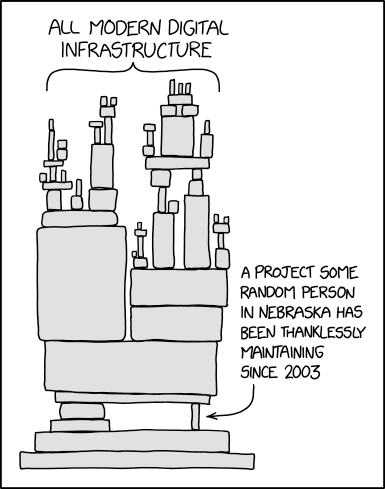
\includegraphics[width=0.5\linewidth-0.5\columnsep]{images/dependency.png}\hspace*{\columnsep}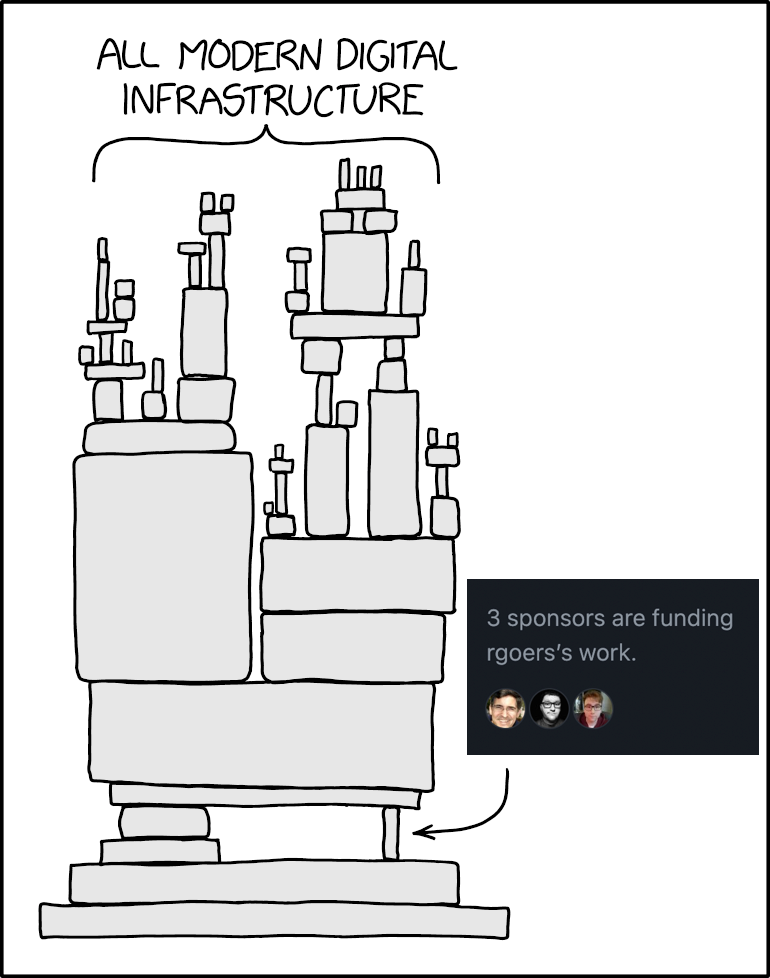
\includegraphics[width=0.5\linewidth-0.5\columnsep]{images/sponsors.png}
  \caption{\label{fig:log4j_dependency}A well-known \texttt{xkcd} meme about modern days software, and a variation of it created specifically for the \texttt{log4j} security breach.}
\end{figure*}

In such circumstances, it is not so surprising that quality assurances are not a top priority for the maintainer of the code.
Filippo Valsorda, a member of the \texttt{golang} team at Google, wrote on this topic that \textcquote{filippo_valsorda_professional_2021}{the role of open source maintainer has failed to mature from a hobby into a proper profession. The catastrophic consequences are almost a daily occurrence. [...] [T]he status quo is unsustainable.}

Maybe open source does not need a business model to survive, live on and thrive, but the world needs open source to have one.

\section{Key Aspects of Open Source}

\subsection{Stakeholders}

In any open source project, there are multiple stakeholders.
The two stakeholders which are always present are:

\begin{description}
  \item[Developers]
  	They create, improve and maintain the project.
  \item[Users]
  	They draw some value from the project.
  	Users can be other developers that use the current project as part of their project, e.g.\ in the case of a software library; or users can be nontechnical people like users of an open source app on a phone.
\end{description}

There is a fundamental imbalance in the open source ecosystem, which is that it is often much easier to get some feedback from developers that know the platforms used to collaborate on code (like GitHub) than it is to get feedback from users.
When users are developers, this is not such a big issue.
But when users are nontechnical, getting some feedback to prioritize the most valuable features can be harder.
Corporate products will often measure in some capacity user behaviors.
This is done much more seldomly in the open source world, first, because it requires a server to receive and store those data for which someone needs to pay (but the projects generally do not make any money), and second because tracking users goes against the open source narrative.
Finding ways to get feedback from the users might make the open source provide more value to humanity.

\subsection{Scales of Open Source Projects}

Open source can operate at various scales.
Many projects have one developer and few users.
Some others attract hundreds of developers and have millions of users like the Python library \texttt{pandas}.

Hereafter we outline three developer community scales that are useful to keep in mind when developing management systems for open source.
Whatever the system, it should adapt well to all three, or it should be specified to which category it applies.

\begin{description}
  \item[Small]
    One to three developers, strong vision, tight coordination, and intentional core design.
    No need for explicit management; it will most probably happen in an organic way, or through the original leader of the project.
  \item[Medium]
    Four to fifteen people, traditional management might bring more benefits than drawbacks at this scale, e.g.\ avoiding duplication of effort, making sure no detail is forgotten, etc.
  \item[Large]
    Management becomes unmanageable.
    Better to embrace anarchy at this point.
\end{description}

\subsection{Core and Halo Developers}

Open source relies strongly on its developer community to make progress.
Yet, not all developers contributing to the project are equal.
Some are more involved, others are less.
As proposed in \citetitle{raymond_cathedral_2001}, developers can generally be divided into two categories:

\begin{description}
  \item[Core]
  	Those are the developers which are highly involved in the project.
  	They generally know the codebase well and contribute regularly.
  	Being at the center of the project, they often coordinate the project in some way.
  \item[Halo]
  	Halo developers are those that contribute a couple of times, maybe only once.
  	They have a specific feature that they want to be implemented or a bug that they want to be fixed.
  	However, they generally don't know the codebase well and it might be hard for them to know where the feature that they want to build needs to go.
  	Having some guidelines for contributors to help them find their way is often useful.
\end{description}

\subsection{Management Styles}

There are probably as many management styles for open source as there are open source projects.
However, the book called \citetitle{raymond_cathedral_2001} \cite{raymond_cathedral_2001}, a famous essay on this topic, describes the models used by two different projects and uses them as general categories:

\begin{description}
  \item[Cathedral]
    Centralized, one or few leaders that coordinate the work of many subordinates, also called \textit{top-down}.
    Coordination happens \textit{a priori}.
    Access to the project's development might be restricted to only trusted developers.
    The leaders provide/impose their vision for the project.
    Code is released once a coherent set of tested features have been added, which generally happens at fixed deadlines.
    A famous program developed using this framework is GCC, the GNU C Compiler.
  \item[Bazaar]
    No management of who should do what.
    Everyone can contribute, the development process is completely public and somewhat anarchistic, also called \textit{bottom-up}.
    Coordination happens \textit{a posteriori}.
    Code is released continuously, at no set deadlines.
    This model was spearheaded by Linus Torvald, and is still used to develop the Linux kernel.
    This model is probably the most cited reason for the kernel's success.
\end{description}

For the bazaar development style to work efficiently, a large enough base of developers needs to be involved.
\citeauthor{raymond_cathedral_2001} proposes, to bootstrap a bazaar-managed project, that developers be attracted by providing a vision and some working prototype.
Providing a clear vision ensures that only align people take part in the project, in the beginning at least.
Having less aligned people later is much less of an issue that having unaligned people in the beginning, as it causes a lot of disruption.
Further, building a working prototype, even if very poor, gives something tangible that people can play with.
It gives some insight into what the finished product might look like, which helps bring people on board.
The book further postulates that a flat organization with only a few project maintainers for the project's coherence is the better way forward.
The power of a large decentralized community beats a single mind, however brilliant it is.

Note that \citetitle{raymond_cathedral_2001} was written in 1997.
Git was released in 2005, so the book describes a time when mailing lists were used commonly for coordination of software developers and \emph{git did not exist}.

\subsection{\textsc{Snafu} Principle}

Some further argument in favor of having as little hierarchy as possible is named the \textsc{snafu} principle:
\blockcquote{noauthor_snafu_nodate}{True communication is possible only between equals because inferiors are more consistently rewarded for telling their superiors pleasant lies than for telling the truth.}

\textsc{Snafu} predicts a progressive disconnection of decision-makers from reality, which is an argument regularly used by hackers and proponents of flat hierarchies why strongly hierarchical systems often fail.
A fable illustrating the \textsc{snafu} principle is included in \cref{sec:snafu_fable}.

\section{GitHub's Influence on Open Source}

A major actor in the open source ecosystem today is GitHub \cite{noauthor_github_2022}.
The platform was created in 2008 and provides free, centralized hosting of git remotes, plus many social coding features.
The company was acquired in 2018 by Microsoft for \$7.5 billion.

The original vision behind \texttt{git} was not to use walled, single, centralized remotes as we do today.
The initial vision was actually extremely flexible; \texttt{git} should be able to fit any workflow.
This makes using \texttt{git} difficult for newcomers because \texttt{git} can be used in so many different ways.
Of course, humans like simplicity, and so we deeply associated using \texttt{git} with using some socially-enabled remote because it was simpler; so much, so that many people now confuse \texttt{git} and GitHub.
But the design of \texttt{git} makes it possible to collaborate on code using decentralized workflows.
Only, as those workflows are generally more complex both technically and for the mind, they are not widespread.
There are also no mature technical solutions to working in a decentralized fashion on code as of August 2022.
But some projects are trying to implement a decentralized way to collaborate on code using \texttt{git}, like Radicle (see \cref{sec:radicle} for more details).

GitHub's offering was a game changer, it changed the face of open source.
The interface enabled people to build faster, provided new features like \textsc{ci/cd}%
\marginNote{%
  \marginTitle{\textsc{ci/cd}}
  Continuous Integration/Continuous Deployment is an umbrella term that designates many things, but it generally boils down to having some scripts automatically executed every time a commit is made on a git branch, or every time a merge request is initiated.
  This idea is powerful because it enables developers to automate many boring tasks, like executing tests before merging which increases the assurances on code quality a lot.
  This idea can be pushed further, for example, it is possible to package and deploy your code whenever you commit to the release branch.
  In the world of microservices and web-based products, this means that developers can stop worrying about putting their code online: the code hosting platform will automatically execute a script that will do it for them.
}, merge requests%
\marginNote{%
  \marginTitle{Merge Request}
  A \textit{merge request} is a process to submit code for merging on a protected branch.
  The process can include or mandate code proofreading, successful execution of \textsc{ci/cd} pipelines, including tests, and acceptance by a quorum of permissioned members.
  It often also features a discussion thread which enables people to comment on and discuss about the code.
}, issues%
\marginNote{%
  \marginTitle{Issues}
  Issues are threads that people can use to ask for new features or to report bugs.
  It enables getting some feedback from the community and the users, although nontechnical users probably do not use this channel as it often requires a technical background to be used (an account on GitHub, adding some trace of the bug, tagging correctly, abiding by the contributing guidelines, etc.).
}, comments, stars%
\marginNote{%
  \marginTitle{Stars}
  Developers can give a \emph{star} to the repositories that they like.
  This feature created a reputation system for open source repository: many stars indicate a software used and liked by many.
  Having few stars means that the community behind a project is smaller, hence the code might not receive enough attention to provide strong quality assurances.
}, sponsors%
\marginNote{%
  \marginTitle{GitHub Sponsor}
  GitHub Sponsor is a program created by GitHub whose goal is to provide funding to the open source ecosystem.
  Projects can register on the program, then a \enquote{Sponsors} button will appear on the project's page, enabling people to make one-time or recurring donations to the project.
  While the intention is good, the effects of the functionality have so far been negligible.
}, and so it has become the largest database of open source code in the world with more than 40 million public repositories listed.
Because GitHub is used so much, the functionalities provided by GitHub shaped the history of open source development.
People now regularly conflate \texttt{git} and GitHub, are not so sure which of the two provides what functionalities; this is the extent to which GitHub has become the \textit{de facto} standard.

Among the features offered by GitHub is a permission system.
When a repository is created, its initiator originally has every right on it, and others have none.
Afterward, the repository owner can grant various additional rights to GitHub accounts.
Some of the permissions include: pushing to the repository (can be set per branch) and merging branches (can be set per branch too).
This is a centralized approach to permissions, similar to what is used in the corporate world, but it goes somewhat against the narratives associated with open source, like anarchy and decentralization.
More democratic management systems, like voting systems, were never offered by GitHub, and so the recent history of open source never featured decentralized, permissionless, or trustless governance systems.

\section{Trustlessness Open Source}

Why do we care about governance of open source projects being or becoming decentralized?
Because it enables users of the project to trust the project as a whole, even if some members mean harm to the project or its users.
It makes open source trustless, by improving the following properties:

\begin{description}
  \item[Security]
  	More people involved also implies that it will be more difficult to include some adversarial code in the project.
  	One would need to circumvent code reviews so that no one discovers the adversarial code in the codebase in the future.
  \item[Longevity]
		Having more active contributors gives stronger guarantees that the project will live on because it increases the probability that someone will maintain the project in the future.
    If we consider the Linux project, which is highly centralized around Linus Torvald, one might ask what will happen if Linus dies suddenly in a car accident.
    It is possible that the community behind the project finds a new governance process rapidly and the project only suffers a minimal impact.
    But it can also be that the community explodes and we end up with multiple subcommunities, each maintaining their fork of the Linux kernel.
    Are you willing to take such a risk?
    A decentralized approach features better properties in our opinion.
  \item[Faster Progress]
    People are generally more involved in a project if they have a say in it.
		More people involved means more features built, more bugs discovered, more bug fixes, etc.
\end{description}


\chapter{Blockchains}
\label{sec:blockchain}

\section{Blockchain Basics}

The blockchain was invented by to this day anonymous people from the movement called cypherpunk%
\marginNote{%
  \marginTitle{Cypherpunks}
  Cypherpunks advocate for the preservation of privacy through the use of strong cryptography.
  They value privacy as a fundamental requirement of open societies.
  They propose that privacy is achieved by using strong cryptography, which guarantees privacy by mathematical properties.
  This movement started in the 1980s when cryptography was only the thing of states and was heavily guarded as a national secret.
  \marginPar
  Cypherpunks are a \enquote{punk} because they are anti-establishment, against governments, and do not trust the systems already in place.
  They can be related to anarchists.
}, with ideas that tie into anarchy.
Today, blockchain is mostly known as a speculation market, for high price volatility that can make you rich (or poor) overnight, as a new playing field for Wall Street and the riches.
The original goal of the blockchain was to create a new kind of money, i.e.\ cryptocurrencies, that would not be controlled by the state.
Yet today states are regulating cryptocurrencies%
\marginNote{%
  An example of a state trying to regulate the world of cryptocurrencies is given by the United States blacklisting in August 2022 the Tornado cash smart contract.
  The smart contract allowed to make anonymous transactions on Ethereum.
  This was used both to launder money and by privacy-conscious users of Ethereum (all transactions performed on Ethereum are public).
  But what does it mean to blacklist a smart contract?
  The blockchain is immutable, so it is not possible to delete or stop the Tornado smart contract.
  Instead, the United States is requiring exchanges to prevent any transactions with accounts that interacted with Tornado cash.
  So people that interacted with the smart contract are now locked in the blockchain world, i.e.\ they cannot convert their cryptocurrencies into fiat currencies, nor can they add new cryptocurrencies bought using fiat on some exchange to their account.
  As long as cryptocurrencies cannot be used to pay in day-to-day life, this action from the US government has a strong impact on the crypto community.
} and most of them are now looking into Central Bank Digital Currencies (CBDC), i.e.\ digital currencies similar to cryptocurrencies, but fully controlled by central banks.
Blockchain is a strange and varied ecosystem.

Let's first define what a blockchain is; it is an immutable, distributed ledger, an append-only list of transactions shared by many computers.
Modern blockchains also offer computing capabilities through smart contracts and as such are sometimes called world computers, i.e.\ they are not limited to only storing data, they can perform computations also.
The revolution that blockchains brought is that they are digital and mathematical constructs that guarantee that each computer will eventually have the same database as the other computers, \emph{without the need for centralized coordination}.
To achieve this property, blockchains were created in a game-theoretical conscious way that ensures that computers that try to cheat the database lose in the end.
The mathematical tool that was key in enabling this is \emph{public key cryptography}.

Building a digital, append-only, trustworthy ledger is the perfect substrate to build \emph{currencies}.
And so blockchains are most famously known for enabling \enquote{cryptocurrencies}.
One key addition to blockchains of the first generation, i.e.\ Bitcoin, was the ability of blockchain to perform some computations on top of storing data.
This new generation of blockchains, initiated by Vitalik Buterin and the Ethereum blockchain, also called the blockchains of the second generation, enabled a whole new range of applications, like financial services (exchanges, loaning platforms, derivative markets, etc.), gaming-related features, NFTs, etc.

As a technological tool, blockchains are most probably overhyped; they are databases, and databases have existed for a long time, but the world never got so excited about them.
Nevertheless, blockchains feature interesting properties, like being trustless and public by default.
But \enquote{blockchain} is not just a technological creation, it is also a movement.

\section{The Blockchain Movement}

The word \enquote{blockchain} is sometimes abused, and can describe more than only the technological creation.
Sometimes, it is used to describe the ideological movement associated with the technology, so we list some of the core narratives of the movement hereafter.

Some of the core ideas that underpin blockchains are that one must be able to trust none of the entities running the blockchain, yet be able to trust that the outcome of the blockchain will be correct, i.e.\ that only valid will be included, and they will be executed correctly.
This is a property called \emph{trustless}, which was inherited from the cypherpunks and their distrust for everyone, but especially for governments and banks.
We want strong guarantees that the blockchain will be correct, e.g.\ that included transactions were indeed intended by the account from which they emanate, that no account can send money it does not have, etc.
Ideally, we would like to be able to trust the outcome of the blockchain without having to trust any specific entity running the blockchain.
That way, even if some entity running the blockchain tries to take advantage, hack, or otherwise exploit the blockchain, we know the entity will fail, even if we falsely trusted the entity.
This is a strong requirement, and it departs deeply from the current model, which imposes on people to trust states to manage their currency properly, and banks to manage accounts properly.
But if a bank was to slash a few zeroes from your balance, could you do much about it?

Now that trustlessness is established as a desirable property, how do we achieve it?
Without diving into the numerous mathematical and game theoretical details required, let us affirm that \emph{decentralization} is a requirement to obtain trustlessness.
Assume the power over the blockchain is centralized in a single entity%
\marginNote{%
  To be a little more rigorous, assume that a single entity owns at least 51\% of the mining power.
}, then, for the blockchain to have correct outcomes, you need to trust the entity owning 51\% of the power to do the right thing.
This is the so-called 51\% attack.
Because we want to be able to trust no one, it is required that no such entity exists, that the power is \emph{decentralized}.
Actually, the more the power is decentralized, the better because more decentralization means that it is harder for anyone to obtain the required 51\%.

By extrapolating, if we want the power to be distributed among many people, then we might ideally want that each entity has the same power and that no one receives a treatment of favor.
Having some permissions that others do not have is a form of treatment of favor, it is also a way to encode that someone is more trusted than the others.
Creating systems that are \emph{permissionless}, i.e.\ in which there exists no account that has special privileges, is an explicit goal of the blockchain movement.
Yet, especially when it comes to applications being run on the blockchain like a stablecoin, an exchange, or some NFT smart-contract, it is more difficult to build systems that feature no privileged account like an admin account.
The lack of an admin account, also means that if there is a bug in the smart-contract, \emph{no one} has the power to fix the issue.
The same goes for transactions on a blockchain: if you send your money to the wrong account, no one can help you recover it.
The funds are lost for good.

\section{Sybil Resistance}
\label{sec:sybil_resistance}

Most blockchains are pseudonymous, i.e.\ you are anonymous and identified by a pseudonym.
In such contexts, a single actor can own an unbounded number of accounts.

\begin{definition}[Sybil Resistance]
  The property of a system that cannot be exploited by creating a large number of blockchain accounts.
\end{definition}

Attacking a system by creating many accounts is called a \textit{sybil attack}.
Some systems are vulnerable to such attacks.
For example, quadratic voting systems will assign more weight to multiple votes tallying some voting power, than to a single vote with equal voting power.
In such a system, it is advantageous to split your voting power across multiple accounts and make each account vote to maximize your influence when voting.

Generally speaking, voting systems require sybil resistance and cannot assign influence on a \textit{per account} basis as this can easily be exploited\marginNote{%
  Gitcoin, the project that spearheaded quadratic funding (a variant of quadratic voting), and first used it to finance public good projects, fell victim to sybil attacks during its spring 2022 funding round.
}.
Another example is to build a voting system that gives one vote per account.
In such a context, creating multiple accounts yields more voting power, and so the outcome of the vote is probably decided based on who can create the most accounts in a given amount of time.

What are potential mechanisms to provide sybil resistance?
A natural answer for blockchains is to create voting systems in which your voting power is proportional to the amount of a given \textsc{erc20} token%
\marginNote{%
  \marginTitle{\textsc{erc20}}
  \textsc{Erc20}, the acronym for \enquote{Ethereum Request for Comment \#20}, designates an Ethereum smart-contract standard.
  The standard specifies the interfaces that smart-contract should exhibit to implement a fungible token.
  By extension, fungible token are often called \enquote{\textsc{erc20}}.
}
that you own.
If you split your token across multiple accounts, you still own the same amount of token, hence the same voting power.
It is also possible to use \textsc{erc721} tokens%
\marginNote{%
  \marginTitle{\textsc{erc721}}
  \textsc{Erc721}, the acronym for \enquote{Ethereum Request for Comment \#721}, designates an Ethereum smart-contract standard.
  The standard specifies the interfaces that smart contracts must exhibit to validly implement a non-fungible token, i.e.\ a token with some properties that makes it unique compared to any other tokens.
  By extension, non-fungible tokens are often called \enquote{\textsc{erc721}}.
}.
When using \textsc{erc721} tokens, you can create special rules governing the tokens.

How tokens are obtained becomes an important question.
If you can buy the tokens, which is a natural answer for a blockchain---create a liquidity pool for your token on some decentralized exchange and your token can be bought by anyone---then you have effectively built a plutocracy (see \cref{sec:plutocracy}), i.e.\ the richer have more power.

To create a one person–one vote system, you can use non-transferable \textsc{erc721} tokens that you assign manually, which shifts the burden of distinguishing sybils to the entity distributing the tokens%
\marginNote{%
  This strategy was used by Optimism during its first round of retroactive funding.
}
which does not scale well.

On the blockchain, a system that can give at most one token to any human is called \textit{proof of personhood}.
Note that any proof of personhood system needs to provide two guarantees: first, that a given account is indeed owned by a human, and second that this is the only account that the human has registered in the system.
If a single human can register multiple accounts in a proof of personhood system, then the system does not offer sybil resistance anymore.

These systems are attracting a lot of attention, because proof of personhood is a requirement of many systems, like a universal basic income, or many forms of voting systems.
At large in the computer science world, many advocate for changes regarding how we authenticate, for example using passwordless solutions, based on biometric keys for ex\-ample.
The World Wide Web Consortium%
\marginNote{%
  \marginTitle{W3C}
  The W3C is a widely acknowledged entity that creates open standards for the advancement of the web.
  It is the W3C which publishes the standards for \textsc{html}, Javascript, \textsc{css}, and \textsc{svg}, among others.
}, also known as W3C, published in July 2022 a new standard for decentralized identifiers, or DID\marginNote{\url{https://www.w3.org/2022/07/pressrelease-did-rec.html.en}}.

There are some systems on the blockchain trying to implement \emph{proof of personhood} as a primitive on which to build other systems.
This includes, for example, \emph{Proof of Humanity}, \emph{Gitcoin Passport}, \emph{BrightID}, and the more recent \emph{verifiable credential} based systems like \emph{Civic} and \emph{Ontology}.
Most of these solutions are either very recent or unsatisfactory to some degree.
For example, \emph{Proof of Humanity} requires the upload of a video of oneself performing some randomly decided action to prove humanity.
This is privacy damaging as the video must be public, it is not resilient to \textsc{ai} generated videos%
\marginNote{%
  Today, using deep fake technology, it is possible to make fake videos of people saying or doing things.
  This is possible with only a few pictures of the people that should be faked.
  For example: \url{https://www.youtube.com/watch?v=cQ54GDm1eL0}.
}, and does not guarantee the uniqueness of the account.
Bright ID is a combination of a web of trust and some graph analysis.
The graph analysis that is proposed today returns a number that represents the confidence level of the system in the fact that you are a human, which needs to be converted to a binary decision using a threshold with the regular false positive and false negative issues.
Also, while the system might tell whether an account is managed by a real human, it is a harder problem with such an approach to detect multiple accounts managed by the same human.
Finally, Gitcoin passport aggregates multiple other proof of humanity services like \textit{Proof of humanity}, BrightID, and some other sources which are less secure like Twitter, Google, Facebook, LinkedIn accounts, \textsc{poap} (which are \textit{tradable} location-based NFTs), ENS (which anyone can buy) and discord accounts.
So, while it is harder to fool a meta-system like Gitcoin passport, a sufficiently motivated attacker will most surely succeed in doing so.
Proof of personhood is still an unsolved problem on blockchain as of September 2022.

\section{Quadratic Voting}

Quadratic voting is a voting system in which your influence over a vote is equal to the square root of the number of tokens that you voted with.
If you vote with one token, your influence is one.
If you vote with four tokens, your influence is equal to two.
With nine tokens, you get an influence of three.
For such a system to work, there needs to be a cost to the user that is proportional to the number of tokens voted, i.e.\ not to the influence you obtain.

This system allows people to express a degree of preference, while still giving more weight to the mass, than to the opinions of the rich.
To go further, one can use functions that are more sublinear than the square root like the cubic root or even the logarithm.
In the limit, if you take the infinite root, you have built a one account––one vote system.
There is a continuum between preference voting and one account--one vote.

Unfortunately, quadratic voting is \emph{not} sybil resistant.
You are better off by voting one hundred times one token from one hundred different accounts, for a total influence of one hundred, than by voting one time one hundred tokens which will only give you an influence of ten.
This is the major limitation of this voting system today.

\section{Regenerative Finance}

Regenerative Finance, also known as ReFi, is a blockchain-related movement initiated in December 2021 by Kevin Owocki, one of the founders of Gitcoin%
\marginNote{%
  Kevin Owocki wrote a book outlining the principles of ReFi, which we found an enlightening reading: Green Pill \cite{kevin_owocki_green_2022}.
}
.
The core idea behind regenerative finance is to find new ways to incentivize people to behave in ways that benefit the common good.
Public goods are a core interest of ReFi; these include open source projects, and the environment, for example.

Another important narrative of ReFi is the idea of regenerating instead of extracting.
An extractive strategy is defined as any strategy that cannot be sustained over the long run.
For example, humanity uses more\\fossil fuels per time unit than the Earth generates which is an unsustainable strategy; at some point, the reserves will be emptied.
This concept can be generalized, for example to biodiversity, the absence of war, the absence of carbon in the atmosphere, etc.

We find it interesting to generalize the concept of extractive strategies to a moral, i.e.\ to designate as \enquote{bad} extractive actions.
Burnouts are the consequence of an extractive strategy regarding rest.
Behaving in a way that leads to burnout becomes \enquote{bad}.
States that use more money than they have, by printing a lot of it, or by loaning it, is an extractive strategy, thus it becomes \enquote{bad}.
How does this integrate with our moral intuitions?
Take for example the French state whose public debt was worth 114\% of its BIP in 2020.
With the Covid crisis, the French state had to spend more money on social insurances like partial unemployment indemnities and various other governmental helps to the population.
With the inflation and the increase in the price of gas in 2022, the French government decided to create a price shield, thus France suffered the least from inflation in Europe.
This is good for French citizens in 2022.
But is this a sustainable strategy?
What happens when the strategy can no longer be maintained?
What about the future French citizens?

Regenerative finance departs from ideas accepted as common knowledge in contemporary philosophy.
For example, doing things that can be sustained over the long run is favored over becoming wealthy as rapidly as possible.
If we were to price in carbon compensations, i.e.\ if we added to the regular price of products the price required to offset all the carbon emissions of the product (production, transport, recycling), it would increase the costs of living a lot.
This means a lower purchasing power, less material wealth, and a diminished ability to \emph{do}.
The marginal happiness brought by material wealth is a decreasing function.
In other words, minimum material wealth is necessary for happiness, but mountains of wealth do not make one more happy.
So why try to have ever more of it?

\section{Blockchain Principles and Open Source}

It is difficult to overstate the importance of open source infrastructure for humanity.
The open source runs the web, runs most of the supercomputers, runs all the smartphones, runs the vast majority of all servers, etc.
Yet, the open source comes without guarantees: licenses always start with a variation of \enquote{this software comes without any guarantees}.
Is it reasonable to depend so much on so little guarantees?
Let's consider the Linux kernel.
By now, many trust Linus to do the right thing, and probably rightly so.
But what if Linus were to die in a car accident?
The reliance of the project on a single person makes the project fragile.
We postulate that it would be better for humanity that open source projects, like blockchains, are \emph{trustless}, i.e.\ that you can trust that the project will keep evolving and that it will not actively try to harm its users, \emph{without having to trust any developer individually}.
Bringing trustlessness to open source is an explicit goal of this work.

And while trustlessness improves nothing to unintentional security issues or bugs, it does solve problems like the hack of the \texttt{event-stream} library: a single developer maintained this important library for free until someone proposed themselves to take over the maintenance of the library.
The original, trustworthy author of the library gave the required permission to the new contributor, which was a nefarious individual that took advantage of the situation to include a worm in the library that leaked seed phrases of cryptowallets.
Fundamentally, all open source projects start in a centralized situation, i.e.\ the person that had the idea and created the repository in the first place will have all the power in the beginning.
But if there was a system that fostered decentralizing this power to other people, the project could become more and more decentralized over time, thus improving its trustlessness (and therefore the trust that we can have in the project without knowing each of the contributors personally).

\null\vfill
\drawBackground
\startBackground
\begin{fullwidth}
  Now that we have explored governance systems, the open source movement, and what blockchains are, we turn our attention to building primitives for the open source using blockchain technology.
  We hope to improve some aspects of open source code building which we describe in the next part.
\end{fullwidth}
\vspace*{2mm}
\stopBackground
\vfill\null



\part{GitDao}

\partSecondPage%
GitDAO%
\marginNote{%
  \marginTitle{DAO}
  A DAO, short for Decentralized Autonomous Organization, is a smart contract hosted on the blockchain that is used to coordinate a community.
  Most often DAOs feature a voting system.
  A typical use case is to use DAOs to govern blockchain-oriented investment funds.
}
is the specification of \emph{blockchain primitives aimed at open source software}.
Note that some of the primitives do not fundamentally require blockchains, and can be created using other technologies.

The primitives described hereafter aim to fulfill specific goals among which:

\begin{description}
  \item[Trustless Open Source]
    We want to make it possible to trust an open source project without having to trust any individual developer in the project so that even if some of them have adversarial intentions, they cannot act upon them.
    Trustlessness is the umbrella goal under which many of the following goal fall.
  \item[Decentralization of Power]
    A requirement for trustlessness.
  \item[Developer Incentivization]
    Incentivizing developers to contribute improves the chances of a project living longer.
    Longevity is a requirement for trustlessness: a project that receives no developer attention is a dead project, with no more bug fixes, and no features added.
  \item[Transparency]
    It improves trustlessness, but also makes it easier for newcomers to join, as they can find information about the project more easily.
  \item[Coordination]
    This includes coordination among developers, to make the work more efficient, but also the coordination between developers and users, so that open source projects can bring even more value to humanity.
  \item[Security]
    Obviously.
\end{description}

\chapter{Decreasing Power Token}
\label{sec:chamber_721}

% path
% ref of figure to create
% list of accounts
% ref of scenario described
% caption end
% footnote
\NewDocumentCommand{\printPowerFunctionGraphs}{O{p} m m m m o o}{%
\begin{figure*}[#1]
  \begin{tikzpicture}
		\begin{axis}[
		  name=tokens_power,
		  enlarge x limits=false,
		  title=Absolute Power per Account,
		  width=\linewidth,
		  height=\textheight/6,
			xlabel={$t$},
      ylabel={$p_u(t)$},
			ymin=0,
		]
      \foreach \account in {#4}{
        \addplot table {data/#2/absolute/\account.dat};
        \addlegendentryexpanded{Account \uppercase{\account}}
      }
		\end{axis}
		\begin{axis}[
		  at={(tokens_power.below south west)},
		  yshift=-3mm,
		  anchor=above north west,
		  ymin=0,
		  ymax=1,
		  stack plots=y,
		  area style,
		  enlarge x limits=false,
		  title=Relative Power per Account,
		  width=\linewidth,
		  height=\textheight/6,
		  xlabel={$t$},
      ylabel={$q_u(t)$},
		]
		  \foreach \account in {#4}{
        \addplot table {data/#2/relative/\account.dat} \closedcycle;
		  }
		\end{axis}
  \end{tikzpicture}
  \caption{%
  	\label{#3}%
    \cref{#5}\IfValueT{#6}{ #6}%
  }%
  \IfValueT{#7}{%
    \floatfoot{#7}%
  }%
\end{figure*}
}

In this chapter, we propose a new kind of governance token based on the \textsc{erc721} standard: Decreasing Power Token (\textsc{dpt}).
Those tokens are aimed specifically at governance, and we summarize why we think they fulfill this purpose better than existing solutions at the end of the chapter.

\section{\textsc{Dpt} Properties}

\textsc{Dpt}s feature the following properties:

\begin{description}
  \item[Initial Value Rewards Value Provided]
    The initial value of a \textsc{dpt} must be proportional to the value provided to the project during a given time or through a given task.
    A natural moment to award such tokens in the context of open source is at the end of a merge request.
    A scheme to determine the value of the token is proposed in \cref{sec:rewarding_scheme}.
  \item[Non-transferable]
    Once a token is awarded to an account, it can never be transferred to any other%
    \marginNote{%
		  Non-transferability of tokens that implement the \textsc{erc721} standard, is achieved by throwing some exceptions in all the transfer functions required by the standard.
		  This effectively renders any transfer function from the standard unusable.
		}.
  \item[Decreasing Power]
  	The voting power of a token decreases over time.
  	This encodes the fact that you are probably more involved in a project if you contributed recently than if you contributed a long time ago, as projects evolve.
\end{description}

The power of any user $u$ at time $t$ is given by:

\begin{equation}
  \label{eqn:power_of_user_with_decreasing_erc721}
  p_u(t) = \sum_{\tau\in T_u(t)}\tau\mathtt{.power}(t)
\end{equation}

The formula above is very similar to \cref{eqn:power_in_token_based_voting_systems} but the power of a token now additionally depends on the time $t$.

We use the \textsc{erc721} standard, because it is the most minimal standard that is both widely accepted and that provides enough flexibility to store the information required for \textsc{dpt}s.

\section{Decreasing Power Functions}

In this work, we will restrict ourselves, for simplicity, to decreasing functions composed of two additive terms.
One of the terms is decreasing in time, we call it the \emph{variable power}.
For a given token $\tau$, we denote the initial value of the variable power $v_\tau$.
We reserve the variable $a_\tau$ to describe the speed at which the token decreases in any form meaningful for the specific decreasing function used.
We defined the second term of the power of a token to be a constant.
We call it the asymptotic power, as it is the power that remains when the variable power reaches zero, which might happen at $t=\infty$, and denote it $b_\tau$.

The power at mint time is given by $\tau\mathtt{.power}(t_{mint}) = v_\tau + b_\tau$, and the power remaining in a token at $t=\infty$ is $\lim_{t\rightarrow\infty}\tau\mathtt{.power}(t) = b_\tau$.

For any decreasing power function, it is important to analyze how \emph{relative} powers of users $q_u(t)$ evolve, as it is the metric that matters when voting: it determines the impact you have on the DAO.

Asymptotic power is explored in \cref{sec:asymptotic_power}, while some possible decreasing functions are analyzed in \cref{sec:analysis_of_possible_decreasing_functions}.

\section{Asymptotic Power $b$}
\label{sec:asymptotic_power}

The asymptotic power denoted $b_\tau$ is the long-term memory of a token about the value of the contribution provided by its owner.
We examine a few strategies to set the value of $b_\tau$.

\subsection{Absolute Value Asymptotic Power}

\begin{proposition}[Absolute values for $b_\tau$ do not make sense]
  Assume that all tokens have the same absolute value $b$.
  If no new contributions are made for a long time, then all variable power might reach zero value.
  At this point, each person's remaining power will be proportional to the \emph{number} of tokens obtained, not to the value provided.
  We deem this an undesirable outcome.
\end{proposition}

We conclude that it is better to define the asymptotic power as a \emph{percentage} of the total initial power.
But what percentage should we use?

\subsection{Zero Asymptotic Power}
\marginElement{%
  \null\hfill%
  \begin{tikzpicture}[
      every nodes/.style = {
        font=\scriptsize,
      },
    ]
    \graph[
      layered layout,
      grow down,
      branch right,
      edges={
        nodes={
          sloped,
        }
      },
    ] {
      Can variable power reach $0$? ->["yes"] "$b_\tau \ne 0$";
      Can variable power reach $0$? ->["no"] Anything is fine;
    };
  \end{tikzpicture}\hfill\null%
}

Can we set the asymptotic power to zero?
Must we set the asymptotic power to zero?

We need to know whether the \emph{variable} power can reach zero.
In the case of exponential decay, the answer is no, and so token holders will always keep some power from the contributions they made.
In turn, this means that there will always be some power that remains in the DAO.
In this case, we see no restrictions on the asymptotic power.
It can be set to zero, or some non-zero value.

In the case of tokens whose variable power does reach the zero value at some fixed point in time, like linearly decreasing token, if we set the asymptotic power to zero too, then the DAO might end up in a state in which no one has any power over the DAO left.

This voting system is envisioned to be implemented on the blockchain, so \textsc{dpt}s will likely take the form of a smart-contract.
Smart contracts can receive money, which can be useful to incentivize open source projects, which we explore in the subsequent chapters.
What happens when all tokens reach zero value?
Can no one make any decisions for the project anymore?
In such a case the funds would be lost forever, which is undesirable.
Can anyone take control?
But then people might take control of the smart contract only to empty it of its fund, not for the benefit of the project, which is also undesirable.
In any case, we see it more likely that the developers will mint new tokens to themselves (even if they do not produce any new feature), to keep control.
But creating a system that incentivizes its members to hack it is considered undesirable.
So reaching the situation in which no account has any power left is nonsensical, and should be avoided altogether.

\subsection{Optimum Asymptotic Power Value}

What is a reasonable percentage for $b_\tau$?

This is a complex question, which requires analyzing relative power dynamics.
We first take a look at two extreme cases to illustrate what the design space is.

Let's first consider tokens whose power decreases extremely rapidly (though they never actually reach zero).
Assume that the system is so extreme, that if you are the last to obtain a token, you gain dictatorial power.
This implies that power shifts rapidly from one person to the other.
It is a way to give a lot of importance to recency, and no importance to history.
How does a system which gives dictatorial power to a different person every day integrate with our moral philosophy?
Is it a fair system?
Does it provide good guarantees?
To govern an open source system, we deem that such a situation is not desirable.
One reason is that we aim to achieve decentralized power distribution.
No decentralization lowers security guarantees: among the many one-day dictators of the project, one of them will most certainly be an adversarial agent.
Another reason is that power tends to protect and centralize itself.
So, the rewarding scheme used to award new tokens might be abused by the dictator so that they maintain control.

We now consider the opposite case: tokens whose power diminishes infinitely slowly, i.e.\ constant power tokens.
Such tokens are much more common in modern societies, this is how shares of publicly traded companies behave for example%
\marginNote{%
  Why are constant power tokens more common in modern societies?
  One answer is that such tokens are much easier to implement.
  Are they better than \textsc{dpt}s?
  Maybe, but maybe we suffer from familiarity bias when we emit this opinion.
  We recommend that the reader keep an open mind.
}.
As long as no new tokens are created, the relative power of any token remains constant.
Creating new shares dilutes the relative power of previous shareholders.
We do not think that this approach is desirable either for the reasons below.

One reason is that it shrinks the design space for the initiator of a project.
With \textsc{dpt}s it is possible to create tokens whose relative power augments, e.g.\ when the other tokens lose absolute power faster than the current token.

Another reason is power enshrinement.
This system is the opposite of the system described above, which might be proof enough, that stable power tokens enshrine power%
\marginNote{
  To go even further, consider tokens whose value would increase in time.
  In such a situation, being the first to contribute is advantageous because your token will augment during more time than the others, and so there are strong chances that you have the most power.
  Obtaining more power than the first contributors is hard in such a context: power is enshrined.
}.
One can also remark that tokens whose power does not decrease over time do not discount based on the elapsed time since contribution, hence they enshrine power.
We now show more formally, why constant power tokens enshrine power.
When token have constant power, then the total amount of power in a system must be inflationary%
\marginNote{%
  With \textsc{dpt}s, the system might be inflationary (when more power is minted than power decreases), or deflationary (when power decreases faster than it is minted).
}.
Assume that tokens' initial power is drawn from a \emph{stationary} distribution%
\marginNote{
  We deem it desirable that the initial power of tokens comes from a stationary distribution.
  This way, providing the same value in the past, now, or in the future, brings you the same power over the system.
  It prevents strategic behaviors based on timing, and it simplifies the rewarding scheme because it becomes possible to compare with previous rewards to determine the value of a current reward.
}.
When you get a new token, its relative power is obtained by dividing the power of the token by the sum of the power of all the tokens in the system.
If these tokens have decreasing value, then this sum will be smaller, and hence you would obtain more relative power, than in the system with constant power tokens.

This is fundamentally a moral question: for what duration should society concede an advantage as compensation for good deeds.
For example in Switzer\-land, federal counselors, at retirement and provided that they held office for four years at least, benefit from a pension of approximately 225'000CHF per year.
Some are questioning whether it should be abolished.
The state of Geneva abolished in November 2021 the life pension that counselors from the \enquote{Grand Conseil} were entitled to (another effect of the \enquote{Affaire Maudet}).

How important should new contributions be compared to old ones?
We propose that finding a middle ground is the appropriate answer.
Current systems enshrine power too much, making it difficult to bring change, even when many current contributors agree, but a few past contributors disagree.
This makes power transitions too difficult.
For the current system, this means setting $b_\tau$ to percentages that are neither too close to 100\% nor to use percentages too close to 0\%.
Each project is different, so the expectations regarding power entrenchment might vary: some might desire very stable power dynamics, and others might favor a more agile approach.

\section{Analysis of Possible Power Functions}
\label{sec:analysis_of_possible_decreasing_functions}

We now analyze a few decreasing functions to get a feeling of the possible effects of using decreasing power tokens.

\subsection{Scenarios}

For each decreasing function analyzed, we will explore some scenarios, where a scenario is a sequence of mint events.

\begin{scenario}[Identical power at different time steps]
  \label{sce:identical_power_different_time_steps}
  Different accounts receive the same power but at different time steps.

  \begin{center}
    \begin{tabular}{lll}
      \toprule
        \textbf{Time} & \textbf{Receiving Account} & \textbf{Amount of Power}\\
      \midrule
        0 & A & 100\\
        20 & B & 100\\
        40 & C & 100\\
        60 & D & 100\\
        80 & E & 100\\
        100 & F & 100\\
      \bottomrule
    \end{tabular}
  \end{center}
\end{scenario}

\begin{scenario}[Different powers at identical time step]
  \label{sce:different_powers_identical_time_step}
  Tokens of different powers are minted at the same time.

  \begin{center}
    \begin{tabular}{lll}
      \toprule
        \textbf{Time} & \textbf{Receiving Account} & \textbf{Received Amount}\\
      \midrule
        0 & A & 100\\
        0 & B & 80\\
        0 & C & 60\\
        0 & D & 40\\
        0 & E & 20\\
      \bottomrule
    \end{tabular}
  \end{center}
\end{scenario}

\begin{scenario}[Less power later]
  \label{sce:less_power_later}
  An account receives a token of lesser value than another account, but later.

  \begin{center}
    \begin{tabular}{lll}
      \toprule
        \textbf{Time} & \textbf{Receiving Account} & \textbf{Amount of Power}\\
      \midrule
        0 & A & 100\\
        50 & B & 50\\
      \bottomrule
    \end{tabular}
  \end{center}
\end{scenario}

\begin{scenario}[Main contributor]
  \label{sce:main_contributor}
  The main contributor builds half of the features of a project, and various other developers contribute single features.

  \begin{center}
    \begin{tabular}{lll}
      \toprule
        \textbf{Time} & \textbf{Receiving Account} & \textbf{Amount of Power}\\
      \midrule
        0 & A & 100\\
        10 & B & 100\\
        20 & A & 100\\
        30 & C & 100\\
        40 & A & 100\\
        50 & D & 100\\
        60 & A & 100\\
        70 & E & 100\\
      \bottomrule
    \end{tabular}
  \end{center}
\end{scenario}

\subsection{Linear Decay}
\marginElement{%
  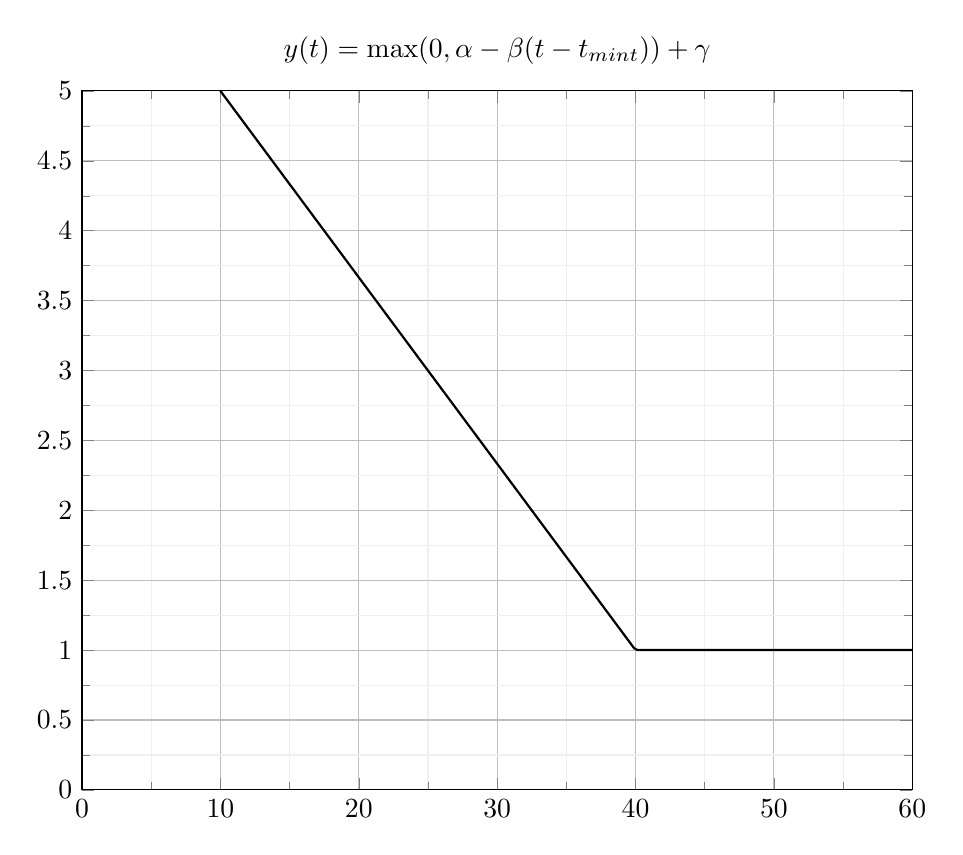
\begin{tikzpicture}
    \begin{axis}[
      xmin = 0, xmax = 60,
      ymin = 0, ymax = 5,
      title = {$y(t) = \max(0, \alpha - \beta (t - t_{mint})) + \gamma$},
      % xtick distance = 2.5,
      % ytick distance = 0.5,
      grid = both,
      minor tick num = 1,
      major grid style = {lightgray},
      minor grid style = {lightgray!25},
      width = \linewidth,
      % height = 0.5\textwidth
    ]
      \addplot[
        domain = 10:60,
        samples = 200,
        thick,
      ] {max(0, -4/30 * (x - 10) + 4) + 1};
    \end{axis}
  \end{tikzpicture}
  \captionof{figure}{\label{fig:linear_decay}Linear Decay}
  \vspace*{\baselineskip}%
  {%
    \small%
    Parameters: $a = \sfrac{4}{30}, t_{mint} = 10, b = 4$ and $c = 1$%
  }
}

Probably the most simple decreasing function to use is the linearly decreasing function.
A visual representation of linear decay is given in \cref{fig:linear_decay}.
The power function of a token $\tau$ is given by:

\begin{equation}
  \label{eqn:linear_decay_power}
  \tau\mathtt{.power}(t) = %
  \begin{cases}
    0 & t < t_{mint}\\
    \max\left(0, v_\tau - a_\tau(t - t_{mint})\right) + b_\tau & \forall t\ge t_{mint}\\
  \end{cases}
\end{equation}

The slope parameter $a_\tau$ of linear decay functions (see \cref{eqn:linear_decay_power}) can be selected in various ways, two of which are intuitive.
One idea is to select the same constant slope for all tokens.
The other is to define an identical duration for all tokens during which they move from their maximal value to their minimal one.

As shown in \cref{sec:asymptotic_power}, it is not possible to use a zero asymptotic power with linearly decreasing tokens.
In all the following examples, we set $b_\tau$ to 50\% of the initial value of the token.

\subsubsection{Constant Slope}

Let's first look at the simplest option, which is to set the same slope for all tokens.
Such a situation is shown in \cref{fig:linear_decay_constant_slope_different_powers_identical_time_step}.

\printPowerFunctionGraphs[ht]%
  {different_powers_identical_time_step/linear_decay_constant_slope}
  {fig:linear_decay_constant_slope_different_powers_identical_time_step}
  {a,...,e}
  {sce:different_powers_identical_time_step}
  [with linear decay with constant slope]

This setup is deemed undesirable because people that obtain tokens with larger values are rewarded doubly: once because their token has large power, and a second time because this power takes a long time to decrease.
If developer rewards are enabled, then the double paying is quite literally happening.

\subsubsection{Constant Time to Asymptotic Power}

\printPowerFunctionGraphs%
  {identical_power_different_time_steps/linear_decay_constant_dt}
  {fig:linear_decay_constant_dt_identical_power_different_time_steps}
  {a,...,e}
  {sce:identical_power_different_time_steps}
  [with linear decay with constant $\Delta t$]

\printPowerFunctionGraphs%
  {different_powers_identical_time_step/linear_decay_constant_dt}
  {fig:linear_decay_constant_dt_different_powers_identical_time_step}
  {a,...,e}
  {sce:different_powers_identical_time_step}
  [with linear decay with constant $\Delta t$]

\printPowerFunctionGraphs%
  {less_power_later/linear_decay_constant_dt}
  {fig:linear_decay_constant_dt_less_power_later}
  {a,...,b}
  {sce:less_power_later}
  [with linear decay with constant $\Delta t$]

\printPowerFunctionGraphs%
  {main_contributor/linear_decay_constant_dt}
  {fig:linear_decay_constant_dt_main_contributor}
  {a,...,e}
  {sce:main_contributor}
  [with linear decay with constant $\Delta t$]

We now consider another approach in which the slope is defined so that the tokens will reach their asymptotic power after a preset time $\Delta t$.
We set this time to 50 time-step in this simulation.
We redefine $a=\sfrac{v_\tau}{\Delta t}$ and remark that this definition satisfies what we are looking for: at $t = t_{mint}$, $\tau\mathtt{.power}(t) = v_\tau + b_\tau$ and at $t \ge t_{mint} + \Delta t$, we have $\tau\mathtt{.power}(t) = b_\tau$.
This setup is illustrated with \crefrange{fig:linear_decay_constant_dt_identical_power_different_time_steps}{fig:linear_decay_constant_dt_main_contributor}.%

In the specific case of tokens with different powers, but minted at the same time, i.e.\ the situation described in \cref{sce:different_powers_identical_time_step}, note that relative powers between these tokens remain identical (\cref{fig:linear_decay_constant_dt_different_powers_identical_time_step}).
This does not hold when the token are minted at different time steps however (see \cref{fig:linear_decay_constant_dt_identical_power_different_time_steps}).

We do not see obvious problems with the results of linearly decreasing power tokens with constant time to asymptotic power.
Some real-life experimentations are required.

\subsection{Exponentially Decreasing Function}

\leavevmode\marginElement{%
  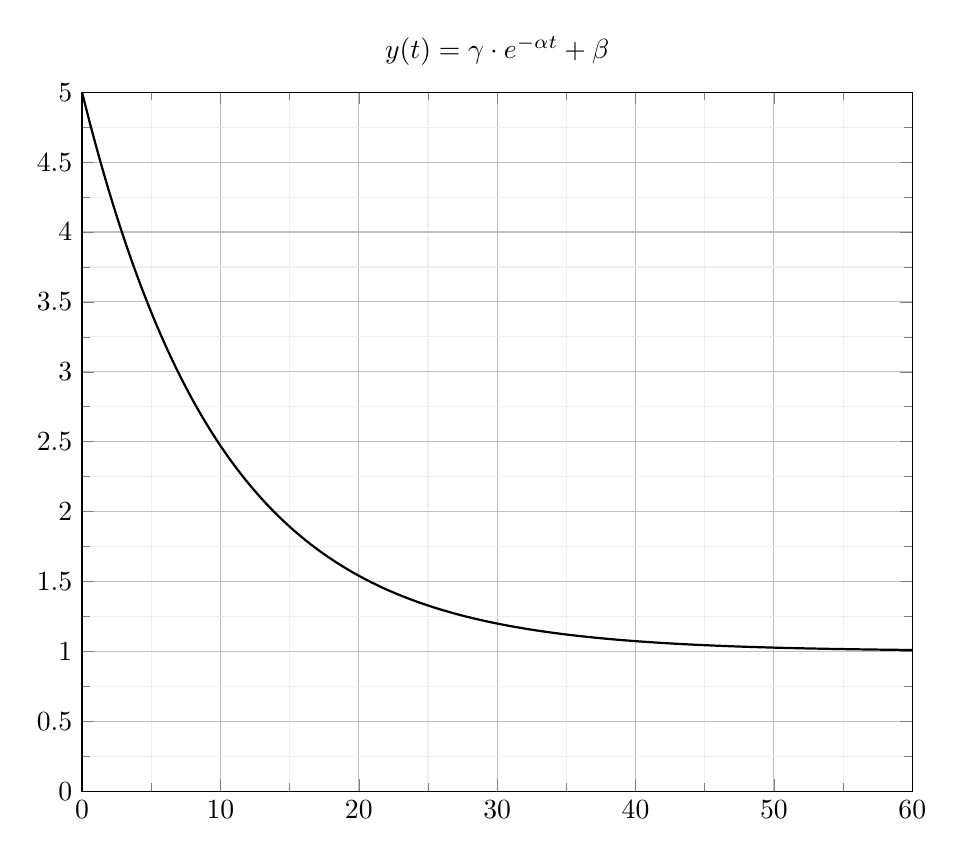
\begin{tikzpicture}
    \begin{axis}[
      xmin = 0, xmax = 60,
      ymin = 0, ymax = 5,
		  title = {$y(t) = \gamma \cdot e^{-\alpha t} + \beta$},
      % xtick distance = 2.5,
      % ytick distance = 0.5,
      grid = both,
      minor tick num = 1,
      major grid style = {lightgray},
      minor grid style = {lightgray!25},
      width = \linewidth,
      % height = 0.5\textwidth
    ]
      \addplot[
        domain = 0:60,
        samples = 200,
        smooth,
        thick,
      ] {4 * exp(-x/10) + 1};
    \end{axis}
  \end{tikzpicture}
  \captionof{figure}{\label{fig:exponential_decay}Exponential decay}
  \vspace*{\baselineskip}%
  {%
    \small%
    Parameters: $\gamma = 4$, $\alpha = \sfrac{1}{10}$ and $\beta = 1$%
  }
}%
Exponential functions come up rather frequently in nature, so it might be a worthwhile function to explore.
A visual representation of exponential decay is given in \cref{fig:exponential_decay}.
Below is the mathematical formula of the power of an exponential decay \textsc{erc721} token $\tau$:

\begin{equation}
  \label{eqn:power_of_exponential_decay_erc721}
  \tau\mathtt{.power}(t) = v_\tau \cdot e^{-a'_\tau (t - t_{mint})} + b_\tau
\end{equation}

A disadvantage of exponential decay functions is that they are harder to understand for humans, which makes the system more complex.

We define $a_\tau$ as the half-life of the function, i.e. the time after which the value of the function is halved.
For a half-life of $5$ time units, the coefficient $a'_\tau$ in the exponential must satisfy $a'_\tau = \sfrac{\ln(2)}{a_\tau} = \sfrac{\ln(2)}{5}$.

\subsubsection{Exponential Decay with Zero Asymptotic Power}

\printPowerFunctionGraphs%
  {identical_power_different_time_steps/exponential_decay_30_0}
  {fig:exponential_decay_30_0_identical_power_different_time_steps}
  {a,...,e}
  {sce:identical_power_different_time_steps}
  [with exponential decay with $a_\tau=30$ and $b_\tau=0\%$]

\printPowerFunctionGraphs%
  {different_powers_identical_time_step/exponential_decay_30_0}
  {fig:exponential_decay_30_0_different_powers_identical_time_step}
  {a,...,e}
  {sce:different_powers_identical_time_step}
  [with exponential decay with $a_\tau=30$ and $b_\tau=0\%$]

\printPowerFunctionGraphs%
  {less_power_later/exponential_decay_30_0}
  {fig:exponential_decay_30_0_less_power_later}
  {a,...,b}
  {sce:less_power_later}
  [with exponential decay with $a_\tau=30$ and $b_\tau=0\%$]

\printPowerFunctionGraphs%
  {main_contributor/exponential_decay_30_0}
  {fig:exponential_decay_30_0_main_contributor}
  {a,...,e}
  {sce:main_contributor}
  [with exponential decay with $a_\tau=30$ and $b_\tau=0\%$]

The situation with exponential decay and no asymptotic power is described in \crefrange{fig:exponential_decay_30_0_identical_power_different_time_steps}{fig:exponential_decay_30_0_main_contributor}.%

Exponential functions with zero asymptotic power and identical half-lives have identical relative decreases over the same period.
So given that no mint event occur, i.e.\  $T(t_0) = T(t_0 + \Delta t)$, the relative power $q_u(t)$ of every user $u$ will remain identical between $t_0$ and $t_0 + \Delta t$.
This effect can be witnessed in \cref{fig:exponential_decay_30_0_different_powers_identical_time_step}.
Here is a quick proof:

\begin{equation*}
  \begin{aligned}
    q_u(t_0 + \Delta t) &\overset{\ref{eqn:relative_power}}{=} \frac{p_u(t_0 + \Delta t)}{\sum_{v\in U}p_v(t_0 + \Delta t)}\\
    &\overset{\ref{eqn:power_of_user_with_decreasing_erc721}}{=} \frac{\sum_{\tau\in T_u(t_0 + \Delta t)}\tau\mathtt{.power}(t_0 + \Delta t)}{\sum_{\tau\in T(t_0 + \Delta t)}\tau\mathtt{.power}(t_0 + \Delta t)}\\
    &\overset{\ref{eqn:power_of_exponential_decay_erc721}}{=} \frac{\sum_{\tau\in T_u(t_0+\Delta t)}p_\tau\cdot e^{-a'_\tau (t_0 + \Delta t)}}{\sum_{\tau\in T(t_0+\Delta t)}p_\tau\cdot e^{-a'_\tau (t_0 + \Delta t)}}\\
    &= \frac{\sum_{\tau\in T_u(t_0+\Delta t)}p_\tau\cdot e^{-a'_\tau t_0}\cdot e^{-a'_\tau\Delta t}}{\sum_{\tau\in T(t_0+\Delta t)}p_\tau\cdot e^{-a'_\tau t_0}\cdot e^{-a'_\tau\Delta t}}\\
    &= \frac{\sum_{\tau\in T_u(t_0)}p_\tau\cdot e^{-a'_\tau t_0}}{\sum_{\tau\in T(t_0)}p_\tau\cdot e^{-a'_\tau t_0}}\\
    &= \frac{p_u(t_0)}{\sum_{v\in U}p_v(t_0)}\\
    &= q_u(t_0)
  \end{aligned}
\end{equation*}

This means that it is possible to replicate the semantics of constant value token, i.e.\ relative power that remains identical as long as there are no mints, yet to provide some advantage based on the recency of the contribution.
The size of the advantage is fixed by $a_\tau$.
\Cref{fig:exponential_decay_30_0_identical_power_different_time_steps_comparison} which depicts the relative power of each users at $t=100$ and $t=200$ highlights this.
On the one hand, the users that made contributions more recently have more power than those that contributed longer ago.
On the other hand, the relative power relationships remain constant over time as long as there are no new mints, and indeed the two pies are identical.

\begin{figure*}[ht!]
  \centering
  \begin{tikzpicture}
    \path[%
      /DiagCirc/.cd,
      value list={6.5/A, 10.3/B, 16.3/C, 25.8/D, 41.1/E},
      diagram,
    ];
    \node[
      anchor=south,
    ] at (0, 3.2cm) {$t=100$};
	\end{tikzpicture}
  \hspace*{10mm}%
  \begin{tikzpicture}
    \path[
      /DiagCirc/.cd,
      value list={6.5/A, 10.3/B, 16.3/C, 25.8/D, 41.1/E},
      diagram,
    ];
    \node[
      anchor=south,
    ] at (0, 3.2cm) {$t=200$};
  \end{tikzpicture}
  \caption{%
  	\label{fig:exponential_decay_30_0_identical_power_different_time_steps_comparison}%
    Relative power at $t=100$ and $t=200$ in \cref{sce:different_powers_identical_time_step} with exponential decay and no asymptotic power.
  }
  \floatfoot{%
    All the users in the above pies contributed the same value but at different time steps.
    The recency advantage is rather clear: user F has more relative power than user E, which itself has more than user D, etc.
    Using exponential decay and setting asymptotic power to $0\%$ further implies that relative power relationships remain identical over time, as long as there are no mint events.
    This is showcase above in that the relative power relationships are identical at $t=100$ and $t=200$.
  }
\end{figure*}

\subsubsection{Exponential Decay with Non-Zero Asymptotic Power}

\printPowerFunctionGraphs%
  {identical_power_different_time_steps/exponential_decay_30_50}
  {fig:exponential_decay_30_50_identical_power_different_time_steps}
  {a,...,e}
  {sce:identical_power_different_time_steps}
  [with exponential decay with $a_\tau=30$ and $b_\tau=50\%$]

\printPowerFunctionGraphs%
  {different_powers_identical_time_step/exponential_decay_30_50}
  {fig:exponential_decay_30_50_different_powers_identical_time_step}
  {a,...,e}
  {sce:different_powers_identical_time_step}
  [with exponential decay with $a_\tau=30$ and $b_\tau=50\%$]

\printPowerFunctionGraphs%
  {less_power_later/exponential_decay_30_50}
  {fig:exponential_decay_30_50_less_power_later}
  {a,...,b}
  {sce:less_power_later}
  [with exponential decay with $a_\tau=30$ and $b_\tau=50\%$]

\printPowerFunctionGraphs%
  {main_contributor/exponential_decay_30_50}
  {fig:exponential_decay_30_50_main_contributor}
  {a,...,e}
  {sce:main_contributor}
  [with exponential decay with $a_\tau=30$ and $b_\tau=50\%$]

The situation with exponential decay and asymptotic power set to 50\% of the initial value of the token is described in \crefrange{fig:exponential_decay_30_50_identical_power_different_time_steps}{fig:exponential_decay_30_50_main_contributor}.%

By setting the asymptotic power to a higher percentage of the total power granted, for example, $b=50\%$, the system gives more weight to historical events, than the case in which the asymptotic power is set to zero.

\Cref{fig:exponential_decay_30_50_identical_power_different_time_steps_comparison} shows that the system first goes through some transitory phase during which more recent contributions are advantaged.
Then, as the variable power of all tokens decreases, the system returns to a situation in which the total power owned by each user is proportional to the value contributed in the entire history of the project.
In a sense, the project gives an advantage to recent contributions if there are some, and otherwise returns to distributing power according to the history of value provided.

\begin{figure*}[ht!]
  \centering
  \begin{tikzpicture}
    \path[%
      /DiagCirc/.cd,
      value list={16.8/A, 17.7/B, 19.1/C, 21.4/D, 25.0/E},
      diagram,
    ];
    \node[
      anchor=south,
    ] at (0, 3.2cm) {$t=100$};
	\end{tikzpicture}
  \hspace*{10mm}%
  \begin{tikzpicture}
    \path[
      /DiagCirc/.cd,
      value list={19.6/A, 19.7/B, 19.9/C, 20.2/D, 20.6/E},
      diagram,
    ];
    \node[
      anchor=south,
    ] at (0, 3.2cm) {$t=200$};
  \end{tikzpicture}
  \caption{%
  	\label{fig:exponential_decay_30_50_identical_power_different_time_steps_comparison}%
    Relative power at $t=100$ and $t=200$ in \cref{sce:different_powers_identical_time_step} with exponential decay and asymptotic power set to 50\% of the initial power of the token.
  }
  \floatfoot{%
    In the first pie, the variable power of the first minted token has largely decreased, but the most recent tokens do not yet have lost this value.
    Thus the most recent contributions are rewarded with more relative power.
    But if no new contributions are made, then the variable power of all tokens diminishes, and the power distribution converges to giving the same relative power to everyone as everyone contributed the same value to the project though at different time steps in this scenario.
  }
\end{figure*}

\section{Are \textsc{dpt} Good for Governance Purposes?}
\label{sec:dpt_philosophical_analysis}

What are the benefits of using \textsc{dpt}s over constant value tokens?
Are there limitations?
We explore these questions in this section.

\subsection{Timing Strategies}

We first consider whether there might exist strategic behaviors that exploit time.
Might actors have incentives to wait before contributing, or is it always better to contribute as soon as possible?
We consider that any project should aim for agents to contribute as soon as possible because it increases the speed of development.

In the following discussion, we define $v_u(t, q_u(t))$ as the private valuation that user $u$ has for owning $q_u(t)$ relative power at time $t$, and $v_u$ as the total value that user $u$ gets over time.
The variable $v_u$ could be called user $u$'s \emph{interest}, as it is the total private value that user $u$ obtains from the power they own over time:

\begin{align*}
  v_u &= \sum_{t=0}^\infty v_u(t, q_u(t))\\
  &= \sum_{t=0}^\infty v_u\left(t, \frac{\sum_{\tau\in T_u(t)}\tau\mathtt{.power}(t)}{\sum_{\tau\in T(t)}\tau\mathtt{.power}(t)}\right)\\
\end{align*}

We keep $q_u(t)$ a parameter of $v_u$, instead of defining, for example, the value per unit of relative power at time $t$ as a constant, because the marginal utility of the relative power might not be constant%
\marginNote{%
  In the case of money, for example, it is generally accepted that for most humans money had a diminishing utility, i.e.\ the more money you have, the less you care about earning an additional dollar.%
}.

Let's first consider the case in which asymptotic power is zero, $b = 0\%$, and assume you know that no one other than you will contribute to the project: $T_{-u}(t_1) = T_{-u}(t)\forall t\ge t_1$, where $T_{-u}$ designates the set of the set of tokens owned by each user, except that of user $u$.
This case, although specific, is interesting, because there might be reason enough to delay a contribution.
In this context, if you contribute later, you get more relative power because the power of the others diminishes when you wait.
This is illustrated in \cref{fig:exponential_decay_30_0_identical_power_different_time_steps}; account E, by contributing later, gets a large share of relative power.
If they had waited for more, they would have gotten even more relative power.
And as we assume that we have oracle knowledge that no other contributions will be made, depending on the decreasing function used by the token, we might keep this large relative power share.
But the period during which you do not contribute must also be considered: having no power during this period has a cost, as illustrated by the equation above which sums over all time steps.
So the situation is not clear and depends on your private valuation for having some power early versus having more power later, and on the decreasing function used.

In projects with no asymptotic power, but in which contributions of similar value are made at regular intervals, contributing early or late does not make a difference.
Through our assumptions, and given that the function used for the tokens decays fast enough, we can also assume that the total amount of absolute power in the system will be approximately constant over time.
Hence, there is no clear incentive to make your contribution early or late, as it will grant you the same amount of relative power over time, irrelevant of the specific moment you contribute.

In projects with non-zero asymptotic power, contributing early in the history of the project is better because of inflation.
In \cref{fig:exponential_decay_30_0_identical_power_different_time_steps} for example, account A, by contributing early, obtains a lot more relative power over the history of the project, than account E.
This means that during the early days of the project, so days 0 to 60 approximately, account A can influence the project a lot.

Even with decreasing power tokens, there is no clear case for the existence of strategic behaviors exploiting timing.
Even if there might exist specific circumstances under which users might have an incentive to wait before contributing, the effect of inflation, the loss of relative power during the period in which you withhold your contribution, and the effect that contributions made after yours will have on your power are all incentives to contribute early and as soon as possible.
Having some amount of asymptotic power, in other words, a little bit of inflation seems to improve guarantees.

Another kind of timing strategy is to vote later than one would have normally done, to have more relative power at the moment of voting.
With \textsc{dpt}s this is possible, as there are situations in which waiting and doing nothing will grant you more relative power.
However, provided that the voting periods are short, and that the time intervals across which tokens decrease in power are long, the effects of such strategies are negligible.

\subsection{Speculation on the Value of Governance Token}

The value of governance power is often hard to estimate, yet, because \textsc{dpt} tokens are non-transferable, there can be no market for them, and they can have no value.
Indeed, if you cannot obtain something, then it makes no sense to talk about the value it would bring you.
This disincentivizes people that would contribute to speculate on the future value of the governance token.
It has indeed been an issue for blockchain-based projects, that people have \enquote{participated} (often in very limited ways), only to obtain some token they hoped the value of would increase over time.
This was the airdrop frenzy.
But these people are seldomly interested in the project or aligned with its ideas.
This is also one of the potential core reasons for the success of the open source: as there is so little monetary incentive to participate, people that do participate often do it because they truly align with the project.

There is a way to hack the non-transferability of the token, namely to use a smart contract as a token holder instead of an Externally Owned Account (EOA).
The smart contract might then sell its voting power to the highest bidder.
The smart contract awarding the tokens could assert that the tokens are only minted to EOA.
This can be counter-acted by selling your voting power using regular off-chain mechanisms.
Setting up such a system implies a lot of friction, so we assume that it is not too likely.

\subsection{Sybil Resistance}

Token-based voting, with fixed-value tokens, is sybil resistant.
We claim that \textsc{dpt}s are also sybil resistant.
An intuitive way to convince yourself of this is that the decreasing functions only use the value of the tokens and time as parameters, and are never related to the account that owns the token.
In a sense, the proposed tokens are self-contained, like \textsc{erc20}s.
We prove this mathematically hereafter.
We define two scenarios, in the first scenario user $u$ has only one account that contains all the tokens.
In the second scenario, user $u$ splits their tokens across multiple account that we name $a_0$, $a_1$, ... $a_k$.

\begin{align*}
  \sum_{a_i} q_{a_i}(t) &= \sum_{a_i}\frac{\sum_{\tau\in T_{a_i}(t)}\tau\mathtt{.power}(t)}{\sum_{\tau\in T(t)}\tau\mathtt{.power}(t)}\\
  &= \frac{\sum_{a_i}\sum_{\tau\in T_{a_i}(t)}\tau\mathtt{.power}(t)}{\sum_{\tau\in T(t)}\tau\mathtt{.power}(t)}\\
  &\overset{(1)}{=} \frac{\sum_{\tau\in T_u(t)}\tau\mathtt{.power}(t)}{\sum_{\tau\in T(t)}\tau\mathtt{.power}(t)}\\
  &= q_u(t)\\
\end{align*}

Where equality (1) holds because the absolute power of any token only depends on values relative to the token itself, but is completely independent of the account that holds it.

Defining the decrease of token proportionally to the total amount of power that a person holds enables per person intrinsic progressive decentralization (defined in \cref{sec:governance_system_chamber_721_intrinsic_power_decentralization}) which we deem a desirable goal.
But without some proof of personhood system (see \cref{sec:sybil_resistance}), i.e.\ if we were to use accounts as proxies for persons, this opens the door to sybil attacks.

\subsection{Making Informed Decisions}

One advantage of decreasing power tokens is that they incentivize renewed contributions.
As there is less power entrenchment, either you keep contributing, or you will lose relative power.
In other words, if you have power over the project, then it must be the case that you are actively involved with the project.
This is positive from the perspective of making informed decisions.

\subsection{Incentive to Keep Contributing}

For people that want to keep some control over the project, or for those that want to keep obtaining rewards when developer rewards are enabled, they have an incentive to contribute value actively to the project, otherwise, they will be outshined by newer contributors who will get the larger part of power and rewards.

\subsection{Extrinsic Power Decentralization}

\textsc{Dpt}s, because they entrench power less, are newcomers friendly.
As a newcomer, you have more guarantees that you can rapidly have some impact on the project, than when there is a lot of power entrenchment%
\marginNote{%
  This applies to many systems.
  Compare, for example, your chances, as a newcomer, of impacting a royalty-based system, and a democratic system.
}.
Having low entry barriers drives extrinsic power decentralization.
In this regard, \textsc{dpt}s have better properties than explicit role systems like GitHub (full power entrenchment), and constant value token systems (more power entrenchment than \textsc{dpt}s).

\subsection{Intrinsic Power Decentralization}
\label{sec:governance_system_chamber_721_intrinsic_power_decentralization}

While GitDao might feature extrinsic decentralization, we would prefer that it features intrinsic decentralization as it is a more robust way to decentralize power.
The proposed \textsc{dpt} are akin to a meritocracy, this means that they do not intrinsically distribute power across humans.
Can we build a system that decentralizes power in a per-person fashion instead of per merit?

We postulate that it is impossible to achieve per-person intrinsic progressive decentralization if we lack proof of personhood.
Intuitively, a system cannot use a discriminating property, if it does not know about it.

\subsection{Large and Small Contributions}

The specific decreasing function used might create different incentives when it comes to the size of the contributions.
In the open source, it is generally speaking a good policy to keep contributions small and to create different merge requests for different contributions.
The reason is that it makes reviewing the merge request much more manageable: many small tasks are easier to do than one big task.

Adding many small linearly decreasing tokens with constant time to asymptotic power is identical to creating one large linearly decreasing token with the same time to asymptotic power.
So in the case of linearly decreasing tokens with constant time to asymptotic power, many small contributions or one big contribution grant the same power.

This is not true of linearly decreasing tokens with a constant slope.
In such a case, it is better to create one large token, than to have multiple smaller ones totaling the same initial power, because the larger token will keep some power for a longer time.

When it comes to exponentially decreasing tokens, creating many small tokens or one large token yields identical results.

It might be desirable to look for decreasing functions that incentivize smaller contributions, i.e.\ functions such that the addition of many smaller tokens yields more relative power than one big token, so super-additive tokens.

\subsection{Trust}

We assume that the tokens have a value that is proportional to the value contributed to the project.
Further, those tokens are not transferable.
This means that if you own some tokens, then you must have provided some value to the project.
Assuming that providing said value required some work (which seems a reasonable assumption: no free lunch), then owning a token is proof that you worked for the project.
As such it can be considered that owning a token acts like a trust gate: if you own a token, then you are probably aligned with the project and can be trusted to do what you feel is right for the project.
The trust comes from the fact that if you want to harm the project, then you would probably not benefit the project in the first place by contributing to it.

Large actors like states might have enough resources to finance developers to contribute to a project to gain enough power over the project to be able to harm it in the future.
But performing such an attack is expensive if the power is decentralized enough, the power over the project needs to be maintained, and if an adversarial agent takes over, it is still possible for the community to fork (though forking is not as easy to do when the project has a bank account).


\chapter{Voting Workflow}
\label{sec:governance_system_voting_workflow}

Defining some tokenomics is only the first step toward building a token-based voting system.
We now need to define, in a more detailed way, the voting procedure.
This procedure is important because we can embed more security (or, on the contrary, flaws) in the system.

The trust model underlying the \textsc{dpt}s is that if you have some, then you are trustworthy and have the project at heart.
This probably holds for most contributors as getting a contribution accepted requires investing time and effort.
This might not hold for powerful/rich/motivated actors, however.

On-chain governance systems have an interesting property: as long as the proposal's \emph{outcome} only has \emph{on-chain} impacts, then it can be enforced in a \emph{trustless} way.
The on-chain consequences of the vote can be applied directly by the smart-contract.
This is trustless because the blockchain on which the smart contract is executed is trustless too.
For example, assume that an on-chain voting system is used to decide whether some payment should be done.
If the vote passes, then the smart contract can execute the payment automatically.
Such a strategy is rather common on the blockchain, e.g.\ Maker\textsc{dao} uses such a system to vote and apply in a trustless way modification of some protocol parameters of the DAI stablecoin.
On the contrary, when a trustful governance system is used to decide something, e.g.\ the voting system in Switzerland, the participants of the system must trust that the system will respect the decision and apply it (which has not always been the case, e.g.\ in Switzerland, the Parlament ignored the opinion of the people when it voted on the highly controversial initiative on mass immigration).
Such functionality can also be used for Git\textsc{dao}, for example, to set some parameter of the decreasing power functions, or to accept a merge request.

Consider proposals to make payments.
Being trustless is positive overall, but proposals can also thus become attack vectors.
Adversarial agents can create proposals that would send them all the funds owned by a project, or change some parameters in a way that would damage the community.
Of course, such a blatant attack would surely get voted down, right?
This is where voter fatigue becomes important: how many people are there watching over the project and making sure that accepted proposals are beneficial?

We propose hereafter a voting workflow, based on the \enquote{don't trust, verify} moto.
This workflow applies to binary proposals only.

\section{Proposal Creation}

Only token-holders can start proposals.
We propose that, depending on what the proposal applies to, the creation of such proposals be limited to token holders.

Merge request proposals should be open to anyone, including accounts that do not hold tokens.
Otherwise, If merge requests are limited to people owning tokens, there can never be new contributors.

Proposals that apply to payments or changing parameters of the decreasing function used for the tokens should be restricted to token holders.
This limits Denial of Service attacks, where attackers would create huge amounts of proposals to prevent the project from making any progress.
It also increases security guarantees: some sensible properties of the project can only be modified by members.

\section{Complete Workflow}

Each proposal has two properties: a \textit{trust level} and a \textit{state}.
The trust level indicates how much people trust the content of the proposal to be non-adversarial for the project.
The state property denotes how far in the voting process the proposal is.
The workflow that each proposal follows is described in \cref{fig:governance_system_chamber_721_voting_workflow}.

\begin{figure*}[ht!]
  \centering%
  \scalebox{.65}{%
    \setlength{\x}{3cm}%
    \setlength{\y}{3cm}%
    \begin{tikzpicture}[
      action/.style = {
        ultra thick,
      },
      action label/.style = {
        font=\ttfamily,
        %						fill = white,
        text width = 2.5cm,
        align = center,
      },
      final/.style = {
%					font = \bfseries,
%					text = white,
        fill = lightgray,
        draw = none,
      },
      node distance = 3cm,
      state/.style = {
        rectangle,
        draw,
        ultra thick,
        text width = 2cm,
        align = center,
        inner sep = 2mm,
      },
      time based/.style = {
        dashed
      },
      trust/.style = {
        draw,
        ultra thick,
        inner sep = 4mm,
      },
      trust label/.style = {
        font=\itshape,
      },
    ]
      \node [] (start) at (0\x, 1\y) {Start};
      \node [state] (pending) at (0\x, 0\y) {Pending};
      \node [state] (voting opened) at (0\x, -1\y) {Voting Opened};
      \node [state, final] (canceled) at (-1\x, -1\y) {Canceled};
      \node [state] (voting elapsed) at (0\x, -2\y) {Voting Elapsed};
      \node [state] (finishable) at (0\x, -3\y) {Finishable};
      \node [state, final] (succeeded) at (-0.5\x, -4\y) {Succeeded};
      \node [state, final] (defeated) at (0.5\x, -4\y) {Defeated};
      
      \path [->] (start) edge [action] node [action label, right] {create proposal} (pending);
      \path [->] (pending) edge [action] node [action label, left] {cancel proposal} (canceled);
      \path [->] (pending) edge [action, time based] (voting opened);
      \path [->] (voting opened) edge [action, time based] (voting elapsed);
      \path [->] (voting elapsed) edge [action, time based] (finishable);
      \path [->] (finishable) edge [action] node [action label, left] {finish\\yes $\ge$ no} (succeeded);
      \path [->] (finishable) edge [action] node [action label, right] {finish\\yes $<$ no} (defeated);
      
      \node [trust, fit = (pending) (canceled) (defeated) (succeeded)] (optimistically trusted) {};
      \node [trust label, anchor = south west] at (optimistically trusted.north west) {Optimistically Trusted};
      
      \node (challenged 1) at (1.8\x, 0\y) {};
      \node (challenged 2) at (1.8\x, -1\y) {};
      \node (challenged) at (1.8\x, -1.5\y) [trust label] {Challenged};
      \node (challenged 3) at (1.8\x, -2\y) {};
      \node (challenged 4) at (1.8\x, -3\y) {};
      \node [trust, fit = (challenged) (challenged 1) (challenged 2) (challenged 3) (challenged 4)] (challenged) {};
      
      \path let
      \p1 = (challenged.west),
      \p2 = (challenged 1)
      in [->] (pending) edge [action] (\x1, \y2);
      \path let
      \p1 = (challenged.west),
      \p2 = (challenged 2)
      in [->] (voting opened) edge [action] (\x1, \y2);
      \path let
      \p1 = (challenged.west),
      \p2 = (challenged 3)
      in [->] (voting elapsed) edge [action] node [action label, above=1cm] {challenge} (\x1, \y2);
      \path let
      \p1 = (challenged.west),
      \p2 = (challenged 4)
      in [->] (finishable) edge [action] (\x1, \y2);
      
      \node (challenge elapsed 1) at (3\x, 0\y) {};
      \node (challenge elapsed 2) at (3\x, -1\y) {};
      \node (challenge elapsed) [trust label, align=center] at (3\x, -1.5\y) {Challenge\\Elapsed};
      \node (challenge elapsed 3) at (3\x, -2\y) {};
      \node (challenge elapsed 4) at (3\x, -3\y) {};
      \node [trust, fit = (challenge elapsed) (challenge elapsed 1) (challenge elapsed 2) (challenge elapsed 3) (challenge elapsed 4)] (challenge elapsed) {};
      
      \path let
      \p1 = (challenged.east),
      \p2 = (challenged 1),
      \p3 = (challenge elapsed.west),
      \p4 = (challenge elapsed 1)
      in [->] (\x1, \y2) edge [action, time based] (\x3, \y4);
      \path let
      \p1 = (challenged.east),
      \p2 = (challenged 2),
      \p3 = (challenge elapsed.west),
      \p4 = (challenge elapsed 2)
      in [->] (\x1, \y2) edge [action, time based] (\x3, \y4);
      \path let
      \p1 = (challenged.east),
      \p2 = (challenged 3),
      \p3 = (challenge elapsed.west),
      \p4 = (challenge elapsed 3)
      in [->] (\x1, \y2) edge [action, time based] (\x3, \y4);
      \path let
      \p1 = (challenged.east),
      \p2 = (challenged 4),
      \p3 = (challenge elapsed.west),
      \p4 = (challenge elapsed 4)
      in [->] (\x1, \y2) edge [action, time based] (\x3, \y4);
      
      \node [trust, final, trust label] (blacklisted) at (3\x, -4\y) {Blacklisted};
      
      \path [->] (challenge elapsed.south) edge [action] node [action label, left] {finish challenge\\yes $\ge$ no} (blacklisted);
      
      \node [state] (pending 2) at (4.8\x, 0\y) {Pending};
      \node [state] (voting opened 2) at (4.8\x, -1\y) {Voting Opened};
      \node [state, final] (canceled 2) at (5.8\x, -1\y) {Canceled};
      \node [state] (voting elapsed 2) at (4.8\x, -2\y) {Voting Elapsed};
      \node [state] (finishable 2) at (4.8\x, -3\y) {Finishable};
      \node [state, final] (succeeded 2) at (4.3\x, -4\y) {Succeeded};
      \node [state, final] (defeated 2) at (5.3\x, -4\y) {Defeated};
      
      \path [->] (pending 2) edge [action] node [action label, right] {cancel proposal} (canceled 2);
      \path [->] (pending 2) edge [action, time based] (voting opened 2);
      \path [->] (voting opened 2) edge [action, time based] (voting elapsed 2);
      \path [->] (voting elapsed 2) edge [action, time based] (finishable 2);
      \path [->] (finishable 2) edge [action] node [action label, left] {finish\\yes $\ge$ no} (succeeded 2);
      \path [->] (finishable 2) edge [action] node [action label, right] {finish\\yes $<$ no} (defeated 2);
      
      \node [trust, fit = (pending 2) (canceled 2) (defeated 2) (succeeded 2)] (whitelisted) {};
      \node [trust label, anchor = south west] at (whitelisted.north west) {Whitelisted};
      
      \path let
      \p1 = (challenge elapsed.east),
      \p2 = (challenge elapsed 1)
      in [->] (\x1, \y2) edge [action] (pending 2);
      \path let
      \p1 = (challenge elapsed.east),
      \p2 = (challenge elapsed 2)
      in [->] (\x1, \y2) edge [action] (voting opened 2);
      \path let
      \p1 = (challenge elapsed.east),
      \p2 = (challenge elapsed 3)
      in [->] (\x1, \y2) edge [action] node [action label, above=7mm] {finish challenge\\no $\ge$ yes} (voting elapsed 2);
      \path let
      \p1 = (challenge elapsed.east),
      \p2 = (challenge elapsed 4)
      in [->] (\x1, \y2) edge [action] (finishable 2);
    \end{tikzpicture}
  }
  \caption{%
    \label{fig:governance_system_chamber_721_voting_workflow}%
    State machine of proposals on Git\textsc{dao}.
  }
  \floatfoot{%
    Dashed transition lines mean that the transition occurs automatically after some predefined amount of time.
    Plain lines represent possible transitions, with their name and required conditions if any.
    Italicized state names represent values that the \textit{trust} property can take.
    Normal text state names represent values that the \textit{state} property can take.
    Grayed states are final states.
  }
\end{figure*}

\subsection{Regular Voting Process}

Upon creation, a proposal starts with its trust level set to \texttt{Optimistically Trusted}.
As long as it remains optimistically trusted, the proposal will undergo the following pipeline.

It starts in state \texttt{Pending}.
This period exists to let users read about the proposal, maybe discuss it offline, etc.
As long as it is pending, the proposer can \texttt{cancel} it at no other cost than the transaction costs.
It might make sense for proposers to cancel their proposal, for example, if some better alternative is found or if a bug/security issue is detected in case the proposal is a merge request.

Once the \texttt{Pending} period ends, the proposal will automatically%
\marginNote{%
	On the blockchain, nothing can happen \textit{automatically}.
	In this case, we mean that whatever write transaction is performed on the proposal, e.g. calling the voting function of the contract, the state will first be updated according to the predefined state timeouts.
	Thus, whatever transaction the user performs, the proposition will always be in the correct state.
	This comes at the cost of additional gas consumption for each transaction.
} enter the \texttt{Voting Opened} state.
At this point, a proposal cannot be canceled anymore and token holders are allowed to vote on the proposal.
A token can be used zero or one time to vote on each proposal.
Token holders have three possible actions:

\begin{description}
  \item[Vote in favor] of the proposal if they think the proposal is beneficial for the project.
  \item[Vote against] the proposal if they think it does not benefit the project, but was well intended.
  \item[Challenge] the proposal if they think that the proposal is adversarial, i.e.\ that the proposal was created by someone actively trying to harm the project or its users.
\end{description}

After a predefined duration, the proposal will enter the \texttt{Voting Elapsed} state.
During this period, no state-modifying action on the proposal is allowed anymore.
This gives time to \textsc{dao} members to review passed proposals and potentially challenge them if they deem that they are adversarial.

This \texttt{Voting Elapsed} state prevents attacks in which someone creates an adversarial proposal, hopes that it flies under the radar of the other members of the \textsc{dao}, waits until the last second to vote in favor of the proposal, and finishes the proposal immediately.

When the \texttt{Voting Elapsed} duration is elapsed, the proposal will enter the \texttt{Finishable} state in which anyone can call the \texttt{finish} function which results in the proposal being \texttt{Succeeded} if there is more power assigned to \enquote{yes}, or the proposal being considered \texttt{Defeated} if there is more power assigned to \enquote{no}.
If the proposal is \texttt{Defeated}, then nothing happens.
If a proposal is \texttt{Succeeded}, then the proposal is executed.

The semantic of the votes on proposals is that anyone can hold any opinion without any negative consequences, i.e.\ you can vote with or against the majority.

\section{Challenges}

In any of the non-final proposal states, any token holder can trigger a \enquote{challenge}.
Challenges are a defense mechanism of the \textsc{dao} against adversarial proposals.
The semantics of such votes are however very different: anyone voting against the majority will suffer negative consequences.
Let's first describe how they work.

Once a challenge is triggered, then the proposal enters the trust level \texttt{Challenged} which pauses any regular voting process and opens another voting procedure: the challenge vote.
Token holders can participate in the challenge vote using their governance tokens to indicate whether they consider the challenged proposition to be adversarial (in which case they would vote \enquote{yes}) or not (\enquote{no} votes).
Once the \texttt{Challenged} period times out, the proposal will automatically enter the \texttt{Challenge Elapsed} trust level.
In this state, no action other than calling the \texttt{finish challenge} function is allowed.

If the power assigned in the challenge vote to \enquote{yes} is greater than that assigned to \enquote{no}, then the proposal ends up with the trust level \texttt{Blacklisted}.
This has the following consequences:

\begin{itemize}
  \item 
    All tokens used to vote \enquote{no}, i.e.\ that the proposal was not adversarial, are slashed.
    The idea is that people that say that the proposal is \emph{not} adversarial, while the greater community thinks it is, are probably rogue.
    Only the token used to vote on the proposal are slashed, not all the tokens of the people that voted against the challenge, to provide a little bit of leeway.
    Maybe the people that voted against the challenge did not read the challenge carefully enough, or the interface was confusing and they voted the opposite of what they wanted to vote.

  \item 
    The account that initiated the proposal---\textit{not} the challenge---is blacklisted%
    \marginNote{%
      Banning an account is not much of a punishment: you can simply create a new one.
      The real deterrent is having your token slashed.
    }.
    All its tokens are destroyed and the account is banned from ever interacting again with the \textsc{dao}.
    This is a defense mechanism from the \textsc{dao}: it found a rogue agent, and so it prevents the agent from ever interacting which the \textsc{dao} again in the future.
\end{itemize}

On the other hand, if the power assigned to \enquote{no} is greater than that assigned to \enquote{yes}, i.e.\ the challenge fails, then the proposal reaches the \texttt{Whitelisted} trust level, and the regular voting procedure resumes exactly where it left off.
No further challenge can be requested on the given proposal, to prevent Denial of Service kind of attacks in which a proposal is repeatedly challenged, to prevent it from reaching the \texttt{Voting Elapsed} state.
Additionally, the tokens assigned to \enquote{yes} are slashed.
This creates the incentives necessary to avoid having members use challenges as a second chance to prevent a proposal from being accepted.
Challenges should only be used to flag adversarial behaviors.

Whatever the outcome of the challenge, some tokens might get slashed, and some accounts banned: this is a high-stakes subroutine of the regular voting procedure.

\section{Trust Guarantees}

Some \textsc{dao}s feature systems to increase trust in the outcomes, like quorum.
Why not use one in this voting workflow?
Voter fatigue is a problem for \textsc{dao}s, especially given that voting is generally not rewarded.
Quorums require a lot of effort from \textsc{dao} managers to be achieved.
We want to keep the work overhead induced by GitDAO as low as possible so that it remains valuable even for small projects.

\chapter{Rewarding Scheme}
\label{sec:rewarding_scheme}

There have been multiple strategies used in the history of Computer Science to evaluate how much value employees were contributing to a company.
A notoriously bad strategy is to use the number of lines of code contributed, which incentivizes a coding style that uses as many lines as possible, but which is not correlated to the value of the contribution.

\begin{proposition}[Only Human Can Evaluate the Value Contributed]
  We postulate that the real value of a contribution to a project can only be evaluated by humans, never by some automated metric.
\end{proposition}

This is a somewhat generally accepted idea in software engineering that there is no computationally tractable way to evaluate the value of a contribution.
Consider for example a person that manages code contributors, comes up with ideas, keeps an overview of what everyone is doing to avoid effort duplication, etc. but never contributes code.
That person's contributions are also valuable to the project, but no automated metric based on the code will be able to evaluate it.

In this chapter, we look at schemes that exist and are used to evaluate how much contributors should be rewarded for their work.
Then, we propose a new scheme, targeted at open source projects specifically.

\section{Properties to Fulfill}

We wish to find a rewarding scheme that fulfills the following properties:

\begin{description}
	\item[Proportional Compensation]
		The reward granted should be proportional to the value of the contribution made.
		If you contribute more, you should be rewarded more.
		If all contributions are rewarded equally, then there is no incentive to contribute more.
	\item[Minimum Friction]
		The system should not require too much action from the users, to prevent friction.
  \item[Locally Estimated Value]
    The best people to evaluate the value that some contribution brings are either people close to the effort (those that participated or reviewed the effort) or those that are familiar with similar efforts.
    We mean that it is harder for a computer scientist to evaluate how much work designing a new logo or creating a communication strategy requires than it is for a designer or communication expert.
    Note that this also implies some bias: you are more likely to assign a large reward to pieces of work that are close to your domain of competence because you know how much work it requires.
    But locality might be measured using multiple metrics, not just your affinity to the work produced.
  \item[Trustless]
    The rewarding scheme should not require to trust anyone, even if there are adversarial (but non-colluding) agents%
    \marginNote{%
      This is a strictly weaker guarantee than being able to resist colluding adversarial agents.
      However, colluding adversarial agents is a situation in which it might be impossible to provide any guarantees.
      Also, assuming that adversarial agents do not collude might be a reasonable assumption: there are many ways to behave adversarially, but only one way to behave ethically.
    }.
    A system that features roles, like an admin role, or using any form of permissions, is a system that requires trusting some people to do the right thing and not to abuse their power.
  \item[Explicit Values]
    Rewarding is generally dependent on values: are you rewarding people based on the effort they put in or the effect they achieved?
    How much do you reward people that contributed new ideas versus those that implemented the idea?
    How much do you value people that amplify other contributors?
    Having a process with explicit values is deemed good.
    Value can be intrinsically embedded in the system (which makes it hard to change them), or it can rely on some extrinsic communication among participants to agree on the rewarding values.
\end{description}

\newpage
\section{Case Study: CoordinAPE}

\marginElement{
\includegraphics[width=\linewidth]{images/coordinape.png}}%
In this section, we analyze the rewarding scheme proposed by CoordinAPE \cite{noauthor_coordinape_2022}.

\subsection{CoordinAPE Rewarding Scheme}

CoordinAPE is a tool to evaluate the value provided by members of a \textsc{dao}.
CoordinAPE introduces two concepts: \emph{Circles} and \emph{Epochs}.
A circle is a subset of users of the \textsc{dao} that collaborate.
It is assumed that people inside a circle know well what the other members of the circle are doing.
An epoch is a period of time during which members can evaluate the contributions made by each other member in the circle since the last epoch%
\marginNote{%
  We give here a possible setup.
  Assume that a \textsc{dao} does one-week-long epochs every month.
  This means that members of each circle will have one week to evaluate the work done by other members of the circle in the last month.
}.

At the beginning of each epoch, members of a circle will receive some amount of a token called GIVE.
The amount of tokens that each participant receives is up to the admin of the circle.
Members of the circle can freely distribute the GIVE token to any other member of the circle.
At the end of the epoch, CoordinAPE makes it possible for the \textsc{dao} admin to download a \textsc{csv} file containing how many GIVE each \textsc{dao} participant received.
The value of the payments sent to the contributor is up to the \textsc{dao} admin.
We can assume that the payments are made proportionally, at least to some extent, to the GIVE received.
Note that the amount of GIVE that one can receive depends on the size of the circle one is part of.
So the amount of GIVE received allows discriminating between members of a single circle, but not across circles.

\subsection{Analysis}

\marginBenefit{Locally estimated value.}%
Through circles, CoordinAPE sets up the required tools to estimate value locally.

\marginBenefit{Proportional compensation.}%
Further, the system enables proportional compensations.

\marginDrawback{Not trustless.}%
Yet there are a few limitations to the model proposed by CoordinAPE.
The approach is highly permissioned.
You need an admin to become a member of a circle, you also need an admin to get some GIVE in each epoch, and it is an admin that will perform the payments.
This enshrines power relationships: there are admins, and there are non-admins.
Also, circles are a form of roles.
This makes it harder for people to join and adds friction to any change in status.
There are no guarantees regarding payments.
After each participant assigns GIVE to other members of their circle, the admin might forget to execute the payments or decide that the outcomes of the voting process are not satisfactory, and decide to pay some participants according to their desires.

As noted on CoordinAPE's website, there is some balance to achieve between doing epochs frequently---more user fatigue---and less frequently---but voters suffer from recency bias, i.e.\ they tend to assign more weight to work done recently.
There is also a balance to achieve when it comes to circle size: too many people in a circle and work assessment will be less precise, too few people and the bias of individual voters might become an important factor.

\marginDrawback{Not minimum friction.}%
Because CoordinAPE is not specifically targeted at code-based projects, it cannot use the specific semantics of such projects to its advantage, like merge requests.
For people to know what others have been up to during the last work cycle, CoordinAPE requires that every participant describes in text form the contributions they made.
This represents some additional work for the contributors and introduces some biases in favor of those best able to \emph{sell} the work they accomplished.

CoordinAPE has propositions specifically targeted at open source projects, namely to create two circles: one for the core developers, and a second one for the halo developers.
Halo developers, being generally little involved with a project---they are mainly one-time contributors---, might not constitute a good circle, as they might not be aware of the work that other halo developers are doing (because they are not really involved in the project), and because the circle might be big (there might be a lot of one-time contributor in a project).

Regarding values that should be used in the rewarding scheme, the \textsc{dao} using CoordinAPE is free to specify them, but no specific mechanism is provided in this regard.

\benefitsSummary{%
  \item Proportional compensation (with some potential bias).
  \item Locally Estimated Value.
}[%
  \item Not trustless.
  \item Not minimum friction.
]

\section{Case Study: Valve}
\marginElement{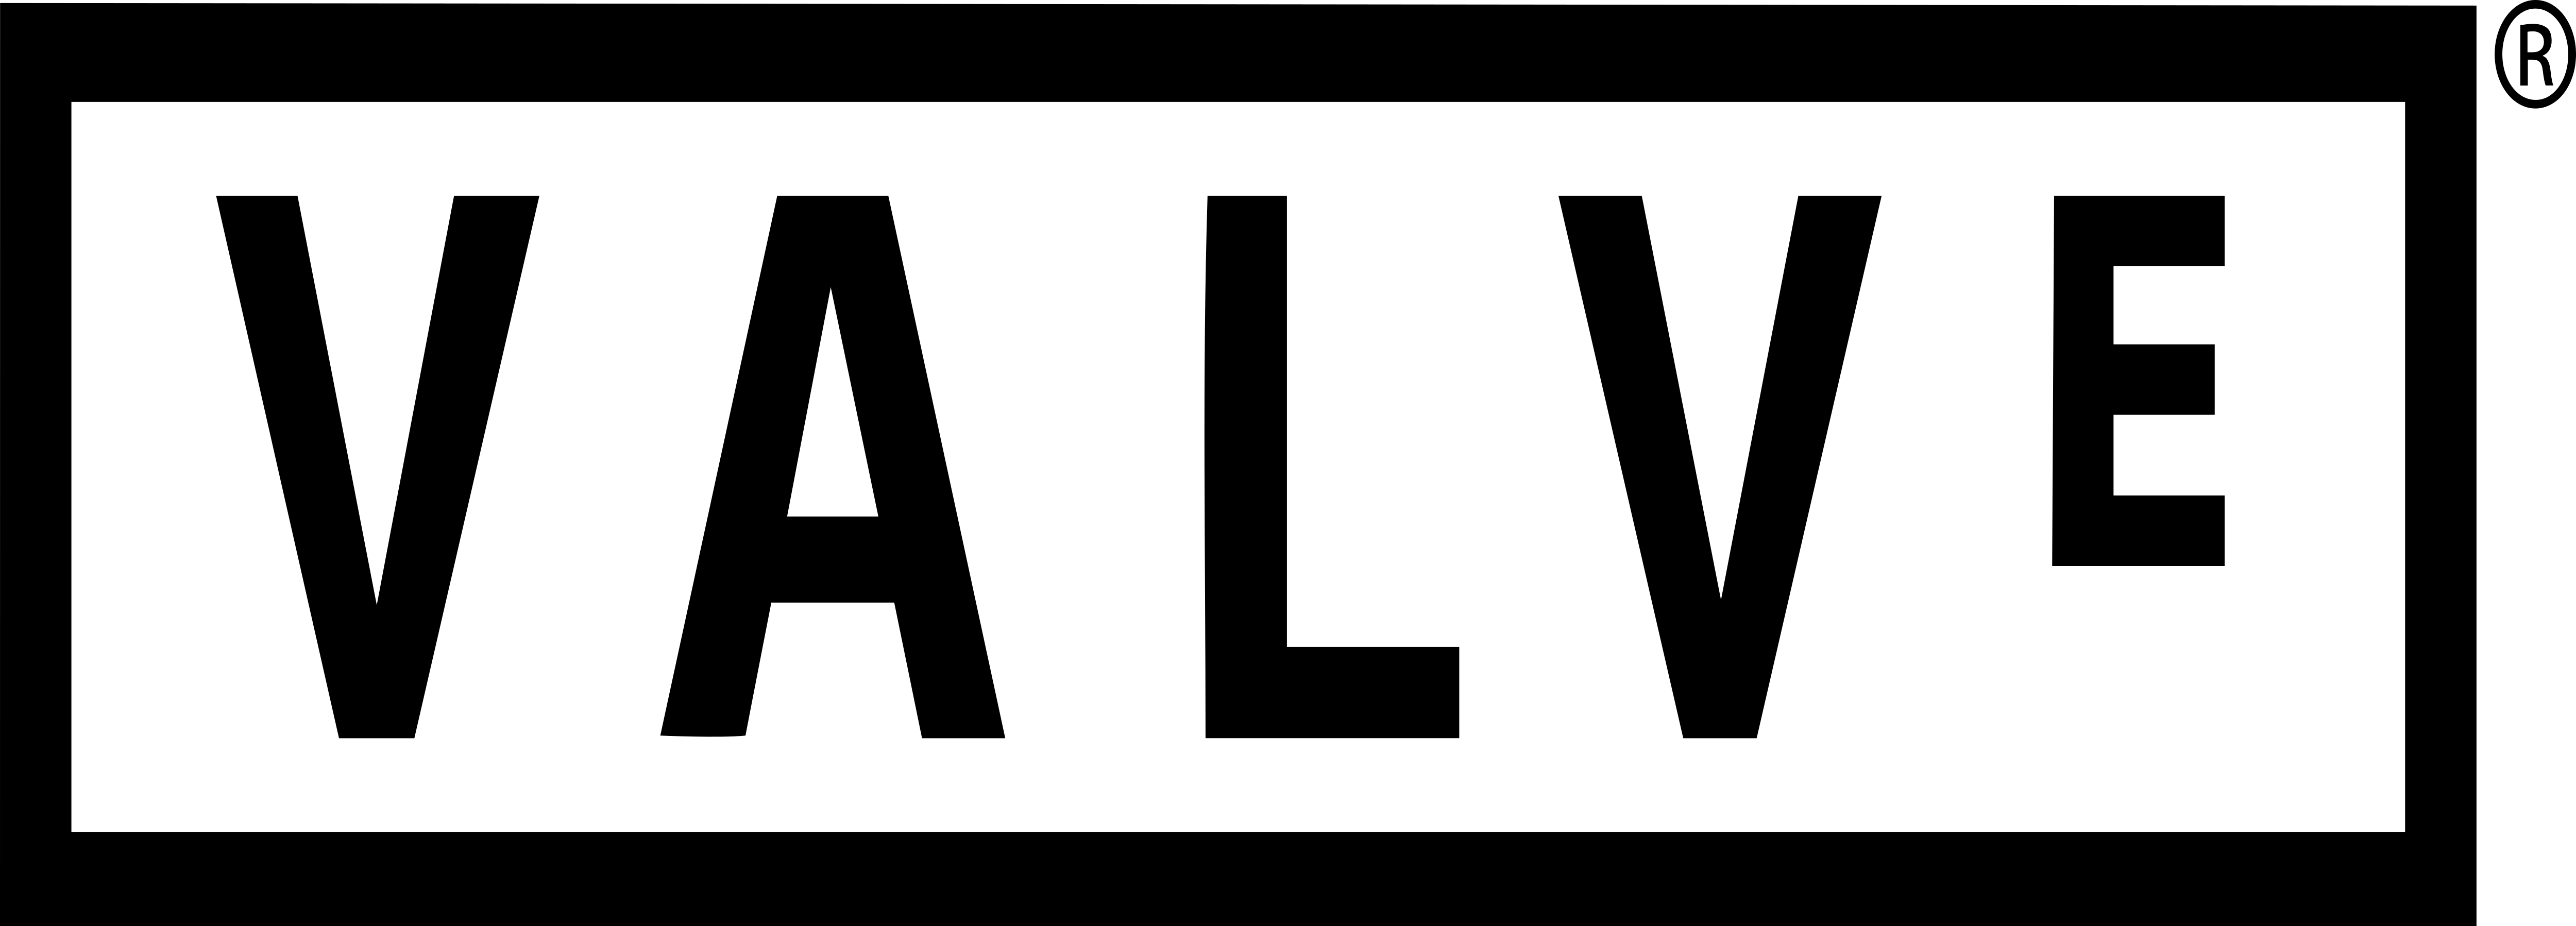
\includegraphics[width=\linewidth]{images/valve.png}}

In this section, we turn our attention to the rewarding scheme used by a famous video game company: Valve.
Valve is the company that created Half-Life (a famous video game), Team Fortress (a famous video game), Counter-Strike (a famous video game), Steam (the most widely used video game platform on PC), Source (a video game engine), Portal (a famous video game), Left for Dead (a famous video game), Dota (a famous video game), and many more.
The company features a fully flat hierarchy described in a handbook \cite{valve_valve_2012} that they give to their employees upon onboarding (unfortunately, the only version we were able to find dates back from 2012).

Valve's explicit policy is to reward employees proportionally to the value they contribute to the company.
In their handbook, they acknowledge that the removal of bias is important and that peers are best suited to evaluate the value contributed by individuals.
As such they have requirements similar to those of a \textsc{dao}, except maybe for the fact that Valve has offices, whereas \textsc{dao}s might happen in a fully remote fashion.
The exact formula used to compute the salary is unfortunately not given but some details are still provided.

This process happens once a year.
\marginBenefit{Locality-based work evaluation.}%
Each employee is asked to rank their collaborators, i.e.\ those people in the company that the individual worked with, on four different criteria:

\begin{description}
  \item[Technical Ability]
    How difficult and valuable are the problems that the collaborator solved?
  \item[Productivity]
    How much shippable, valuable, finished work was achieved by the collaborator?
  \item[Group contribution]
    How much does a collaborator contribute to the group, e.g.\ by hiring people, integrating people into the team, improving workflows, writing tools, or amplifying colleagues?
  \item[Product Contribution]
    How much influence has a collaborator had outside of their core skill domain, for example by prioritizing correctly or predicting precisely how customers will respond to change made?
\end{description}

\marginBenefit{Explicit value criteria.}%
Through this rewarding strategy, Valve makes it clear to its employee what it is that the company values.
Each of the four criteria gets equal weight.

\marginDrawback{Recency bias.}%
Salaries most certainly are proportional, to some extent at least, to the ranking that each employee gets.
This enables proportional compensation, i.e.\ employees are compensated based on the contribution they made during the year to the company.
Conducting the review process once a year implies that the process is a victim of recency bias: assume an employee works a lot in the first six months, then has a kid and starts spending some time at home.
The ranking they will obtain is probably worse than what is fair, because people evaluating them will remember mostly the recent evening during which the colleague went back home, and not the long night that they spent before the birth.

\marginBenefit{No voter fatigue.}%
On the other hand, performing this process once a year only avoids a lot of voter fatigue.
It probably works well for Valve also because they are an on-site company, hence people know each other visually and interact in much deeper ways than what is possible with online communications.
It would be interesting to learn how this process evolved since the 2020 pandemic, or how it would perform in a purely online environment.

\marginDrawback{Not trustless.}%
Valve is not a blockchain-based company, so the voting process is probably conducted on a server from Valve, which requires trusting that the individuals that run the server did not tamper with the data or the computation of each employee's score.
Also, the payments are made by Valve, so the service that performs them needs to be trusted.
Note that the rankings of employees are confidential, so there is no way to check any parts of this system for the employee.

We also remark that Valve produces a lot of code for its video game, but many other types of resources need to be created: sound, visual effects, 2D and 3D assets, animations, etc.
So they cannot exploit the specific semantics of exclusively code-based projects like GitDAO can.

The Valve example highlights that peer-based evaluation schemes can work (Valve is a successful company), and we must not restrict ourselves to simpler systems.

\benefitsSummary{%
  \item Proportional compensation (with potential recency bias).
  \item Locally Estimated Value.
  \item Explicit value criteria.
  \item Minimal friction.
}[%
  \item Not trustless.
]

\section{GitDAO's Rewarding Scheme}

GitDAO focuses on open source code, so we target this proposed rewarding scheme to merge requests.
The rewarding scheme distributes governance tokens, which can be decreasing power tokens, and which can be used by the money distribution process described in \cref{sec:dev_rewards}.

In the context of open source projects, merge requests are a natural workflow to integrate into.
They are required in any case for various reasons, like human proofreading of the code, automated test execution, automated artifacts building, automated deployments, etc.

We propose that once a merge request ends its reviewing process (like comments, fixing typos, refactorings, etc., as defined by the underlying code collaboration stack), people must go through the rewarding scheme to evaluate the rewards to distribute, then the proposal and the rewards are voted on, and if they are accepted, then artifacts are built and deployed.
This pipeline is described in \cref{fig:reward_pipeline}.

\begin{figure*}[ht!]
  \centering
  \setlength{\x}{3.1cm}
  \setlength{\y}{2cm}
  \tikzset{external/export=false}%
  \begin{tikzpicture}[
      process icon/.style = {
        font = \FASolid\fontsize{1cm}{1.2cm}\selectfont,
        text = gray_50,
        anchor = south,
      },
      process/.style = {
        anchor = north,
        align = center,
        text width = 1.5cm,
        font = \small,
      },
      transition/.style={
        thick,
        ->,
      },
      action label/.style = {
        text width = 1.2cm,
        align = center,
        above,
        font = \small\itshape,
      },
    ]
    \node[process icon] (code) at (0\x, 0\y) {\symbol{"F121}};
    \node[process] at (code.south) {Write some code};

    \node[process icon] (review) at (1\x, 0\y) {\symbol{"F530}};%
    \node[process] at (review.south) {Code review};

    \node[process icon] (rewards) at (2\x, 0\y) {\symbol{"F53B}};
    \node[process] at (rewards.south) {Estimate rewards};

    \node[process icon] (vote) at (3\x, 0\y) {\symbol{"F756}};
    \node[process] at (vote.south) {Vote};

    \node[process icon, text = gray_50!70!orange_50] (defeated) at (4\x, 1\y) {\symbol{"F5B4}};
    \node[process] at (defeated.south) {Defeated};

    \node[process icon, text = gray_50!70!green_50] (succeeded) at (4\x, -1\y) {\symbol{"F59A}};
    \node[process] at (succeeded.south) {Succeeded};

    \node[process icon,, text = gray_50!70!red_50] (dead) at (5\x, 1\y) {\symbol{"F54C}};
    \node[process] at (dead.south) {Bad idea or unsalvageable code};

    \path[transition] (code.south east) edge node[action label] {Submit for review} (review.south west);
    \path[transition] (review.south east) edge node[action label] {Submit for rewards} (rewards.south west);
    \path[transition] (rewards.south east) edge node[action label] {Submit for vote} (vote.south west);
    \path[transition] (vote.south east) edge node[action label, sloped] {Vote fails} (defeated.south west);
    \path[transition] (vote.south east) edge node[action label, sloped] {Vote succeeds} (succeeded.west);
    \path[transition] (defeated.south east) edge node[action label] {No new submission} (dead.south west);
    \path[transition, bend right=30] (defeated) edge node[action label, above=3mm, text width = 2cm] {Good code, bad rewards, try estimating rewards again} (rewards);
  \end{tikzpicture}
  \caption{%
    \label{fig:reward_pipeline}
    How rewards are integrated into the merge request pipeline of GitDAO%
  }
  \floatfoot{%
    This figure describes where the rewarding scheme is used during a merge request.
    First people code some functionality, then open a merge request which is proofread by others.
    Any fix is applied before the merge request moves to the reward stage in which people vote on how much each contributor should be rewarded.
    Once the rewards are defined, the merge request moves to a vote.
    If the vote fails, then either the proposers can ask to estimate the rewards again and submit the proposal to a new vote, or they can abandon their merge request.
    If the vote passes, then the code is merged, and the people are rewarded as defined by the rewarding scheme.
  }
\end{figure*}

We propose to split the reward estimation process into two steps:

\begin{enumerate}
	\item
		Evaluate how valuable the merge request is to the project.
		This gives an absolute value to the contribution.
		In the user interface, it would make sense to add other recent features and the value that was granted to those as a baseline.
	\item
		Evaluate the relative contributions of each member that participated in the merge request.
\end{enumerate}

We postulate that it is easier for people to estimate the total value of a merge request%
\marginNote{%
  Estimating the value of something \textit{a priori}, i.e.\ before using it, is often hard.
  Some famous projects, like Gitcoin, propose to evaluate contributions \textit{a posteriori} (through what they call \enquote{retroactive public good funding}).
  In the context of open source software, the problem is not as acute, because the functionalities brought about by a merge request are clear from the code.
}%
and the relative individual contributions separately, than it is to evaluate the individual contributions' value directly.

We denote $\hat v_u(p)$ the estimated value of a merge request $p$, according to user $u$.
We define the aggregated value of the merge request $v(p)$ to be equal to the weighted median of the values $\hat v_u(p)$, which we denote $\weightedMedian(\hat v_u(p))$, and where the weights are given by the relative power of each voter.

Each voter will also need to evaluate the relative contribution of each contributor to the merge request.
We denote $\hat c_u(p, v)$ the contribution that voter $u$ believes contributor $v$ made to the merge request $p$.
Note that the estimated contributions must satisfy $\sum_v \hat c_u(p, v) = 1$.
The aggregated contribution of contributor $v$ on proposal $p$ is:

\[
	c(p, v) = \frac{\weightedMedian(\hat c_u(p, v))}{\sum_v \weightedMedian{\hat c_u(p, v)}}
\]

Each contributor $v$ will receive a governance token with an initial power set to $v(p) \cdot c(p, v)$.

When deciding whether we should use median or mean, we considered the case of an adversarial agent that would vote to assign $100\%$ of the value of a merge request to themselves, for every merge request, even though they contributed nothing.
Of course, we desire that such a strategy yields a reward of zero.
Using the mean would mean that this strategy does yield some rewards every time.
With the median (and given that the adversarial agent does not have 51\% of the power) this strategy is useless.

The proposed pipeline requires that people not only vote on the code, but also on the rewards.
This implies that a vote might fail because rewards did not convince the community and so there needs to be a way to trigger the rewarding scheme again on some given piece of proposed code.
The voting workflow proposed in \cref{sec:governance_system_voting_workflow} only allows binary voting.
So if a vote comes out negative, the proposers of the merge request have no way to know what the reason for the failure was: it might be that the feature is altogether bad, or that the rewards are not appropriate.
This is a problem, but we do not think it is too dire: projects always have some off-chain communication channel (like mailing lists, Slack, Discord, Mattermost, etc.) where proposers can get feedback.
Most probably, the proposer will get feedback way before reaching acceptance or rejection at the \textsc{dao} vote.
Ideally, the platform implementing the GitDAO specification would require people that vote negatively on a proposal to add a comment describing the reason for their vote to allow the proposer to improve and resubmit.

\marginBenefit{Proportional compensation.}%
The scheme allows compensations to be proportional to the value contributed.

\marginBenefit{Locally Estimated Value}%
When looking at merge requests in open source today, most of them are not proofread by the entire community, but only by a few members.
We postulate that to a large extent only the people that wrote the code and those that proofread it will take part in the rewarding scheme.
If this assumption holds, then the value brought by each contributor is evaluated locally.

\marginDrawback{Overestimated value.}
Is there a temptation to overevaluate the total value of the merge request, given that it is the same people that worked on it that will most likely evaluate its value?
Most probably.
But the merge request has to go through a vote by the \textsc{dao} before being accepted, so if its value is overestimated, it risks being rejected, and the proposers will have to go through the rewarding process again.
So people do not have incentives to cheat too blatantly.

\marginBenefit{Minimal friction.}
Proofreading merge requests takes a lot of time, and people do not feel that they create value when doing them.
In turn, this means that proofreading merge requests is rarely an appreciated activity.
Making the process even more burdensome by adding a rewarding scheme to the merge request workflow is a clear limitation of this approach.
If the GitDAO interface uses some heuristic to propose some rewards that people only need to tweak a little bit, so that they match their desire, then the work overload caused by the rewarding scheme might remain bearable.
Further, proofreading a merge request provides some value to the project, e.g.\ security as it ensures that the current merge request is not adversarial, it seems reasonable to reward proofreading merge requests too.
As the proofreading is done before the reward estimation, people should also reward people that conducted useful proofreading.

\marginBenefit{Trustless.}
Note that, as the entire process happens on-chain, including minting the tokens, it is trustless.
There are no roles, there is no one that can prevent you from getting compensated for the work you did for the project.
But what if all of the governance power is held by a single dictator or a few colluding oligarchs%
\marginNote{%
  An open source project must always start in a fully centralized situation.
  Right after it is initiated, the project can have only one contributor: its initiator.
  Hence all the power is centralized in the hands of one person.
}?
Even in such situations, we believe that the system will work well; if GitDAO is used, then the people owning the project want to distribute power over it, so they have little incentive to cheat the rewarding scheme.
Also, if the powerful cheat the system, e.g.\ by appropriating the work of others to themselves, the project would suffer reputation losses, and people might stop funding the project, or the community might fork the project.


\chapter{Developer Rewards}
\label{sec:dev_rewards}

In this chapter, we propose a method to reward developers of an open source project.
The proposed scheme also distributes money to dependencies a project depends on.

\section{Splitting Funds Three Ways}

A smart contract can receive tokens easily, and define callback functions to execute upon receiving them.
We propose that any money received by a project be split three ways upon reception:

\begin{description}
	\item[Developer Rewards]
	  A fraction of the funds received is distributed to developers of the project, proportionally to their governance power in the project at the moment the funds are received.
		
	\item[Further Open Source Funding]
		A fraction of the funds received is redistributed to other open source projects.

	\item[Treasury]
		The remaining part is hoarded up in the treasury of the project, as a reserve that can be used for various other purposes like bug bounties, paying for one-off tasks like branding, or implementing a feature.
\end{description}

This situation is summarized in \cref{fig:money_distribution}.

\begin{figure*}[ht!]
	\centering
	\setlength{\x}{5cm}
	\setlength{\y}{2cm}
	\begin{tikzpicture}[
	    ultra thick,
			money_transfer/.style = {
				->,
			},
			n/.style = {
				align=center,
				rectangle,
				draw,
				text width=2cm,
			},
      main/.style = {
        fill = gray_90,
        draw = none,
        minimum height=2\baselineskip,
				text width=2cm,
				align=center,
      },
		]
		\node[n] (people_donating) at (0\x, -0.5\y) {Blockchain\\Accounts};
		\node[n] (dao_donating) at (0\x, 0.5\y) {Other\\GitDAOs};
		
		\node[main] at (1\x, 0\y) (gitdao) {GitDAO};

		\node[n] at (1\x, -1\y) (token_holders) {Token Holders};
		
		\node[n] at (2\x, -0\y) (dao_receiving) {Other\\GitDAOs};
		
		\path[money_transfer] (dao_donating) edge node[midway, above=4mm] {Donations} (gitdao);
		\path[money_transfer] (people_donating) edge (gitdao);
		
		\path[money_transfer, out=120, in=60, loop] (gitdao) edge node[midway, above] {Treasury} (gitdao);
		\path[money_transfer] (gitdao) edge node[midway, align=left, anchor=west] {Direct\\distribution} (token_holders);
		
		\path[money_transfer] (gitdao) edge node[midway, above, align=center] {Further\\funding} (dao_receiving);
	\end{tikzpicture}
	\caption{%
		\label{fig:money_distribution}
		Money flows in and outside of a GitDAO project.
	}
  \floatfoot{%
    Donations can be received as recurrent donations or one-off donations.
    Donations can come from further funding of other GitDAOs or direct donations from EOA.
		Received money is in part donated to the dependencies of the current project, in part distributed to the token holders of the DAO as remuneration for their work and the value they provided to users, and in part hoarded up, to build the DAO treasury which can be used by the project.
  }%
\end{figure*}

\section{Developer Rewards}

Developer rewards are a way to incentivize developers to contribute to open source by paying them.
Note that the developers do not get a fixed salary out of such contributions.
Rather they obtain a fraction of the funds donated to a project they contributed to when donations are made.
Given enough donations, one can imagine people contributing to open source software as their main occupation, although the uncertainty related to an income being dependent on donation might be a deterrent.

\section{Open Source Funding Graph}

Today, in the open source ecosystem, only the most user-facing projects can live off of donations (like the Mozilla Foundation for example).
Projects less visible receive no attention or donations, most of the time, they do not even have a donation system in place.
Creating smart contracts for each open source project would make it much easier to donate to a project.

Supply chain attacks are becoming more standard on the blockchain.
This highlights the fact that an open source project has some incentive to ensure that its dependencies are properly maintained over time.
From the perspective of the incentives, it makes sense for a project to donate to its dependencies, because the project has an interest in having its dependencies strive: for improved features, rapid bug fixes, documentation, code quality, etc.
If the dependencies are abandoned, a project will have to replace them or take over their development.
By donating a percentage of the funds that an open source project receives to its dependencies, it improves its security guarantees.
Each project can freely choose what percentage of received funds to give to further open source projects.

Allowing money to flow from one project to another creates a \textit{funding graph}.
We remark that this prevents only the most visible projects, e.g.\ Firefox, get all the donations.
It brings donations down in the open source infrastructure stack, to core software pieces that are hidden from sight, yet highly important, like the \texttt{libc}.

\section{Treasury}

Smart contracts make it easy to store money, and so the money received by a project that is not directly distributed to the developers nor sent to further open source projects can be hoarded in a treasury.
Owning a treasury makes an open source project into a full-featured \textsc{dao}.
This money can be used for various purposes, like bug bounty programs.

\section{Streaming Payments and Radicle Drips}

\marginElement{%
  \null\hfill\includesvg[width=.5\linewidth]{images/radicle_drips_logo.svg}\hfill\null\\[1mm]%
  \includesvg[width=\linewidth]{images/radicle_drips_banner.svg}\\[2mm]%
  At \href{https://www.drips.network}{drips.network}%
}
Radicle provides a blockchain protocol for streaming payments.
Streaming payments are the opposite of discrete payments.
So instead of paying a sum in one transaction, the protocol transfers the value small amounts by small amounts at frequent intervals, like every second or so.

This protocol would be perfectly suited for donations in the open source, as it would allow funds to accrue progressively which prevents many kinds of strategic behaviors.
An example of strategic behavior exploiting discrete payments is for a contributor to submit a merge request at the moment in time that guarantees they will receive their token from the rewarding scheme just before a large recurrent monthly donation is made, to have the largest relative power possible over the \textsc{dao}, to maximize the percentage obtained from the donation.

\section{Voting on Parameters}

We propose that each DAO can vote on the specific percentages according to which received donations should be split.
Highly visible projects, e.g.\ user-facing projects, will most probably both receive more donations and use a lot of dependencies.
From the ecosystem perspective, it would be beneficial that they distribute a larger part of their donations to other GitDAOs.
From the project perspective, it might also be a sensible action: the project needs its dependencies to be maintained.
For projects at the absolute bottom of the tech stack, e.g.\ the standard C library, further distribution makes no sense (unless people maintaining the project want to help some other project they care about).
%

\chapter{Issue Backing}
\label{sec:issue_backing}

In this chapter, we propose an additional mechanism for GitDAO.
The goal of this mechanism is to provide funding for issues.

\section{Issues}

\emph{Issues} are inherited from GitHub.
The word describes a forum-like text-based thread that users can use to report bugs, or ask for new features.
Discussions often happen in those issues, to request additional details, about the best way to solve the bug or the best implementation of the requested feature.

However, issues today do not incentivize developers in any way.
So whether the issue is solved depends on developers taking up some of their free time to do it.
We propose a system to incentivize the solving of issues.

\section{Mechanism}

Assume that some user opens an issue.
In the issue, the user describes the bug that they want to be fixed or the feature they want to be added.
Then, the user backs the issue with some amount $\alpha$ of money.
If and when the issue is solved, the project will get the stacked money \emph{discounted by time}.
So the longer an issue awaits unsolved, the less money a project will obtain from solving the issue.
The specific function used to describe the discount can be any decreasing function.
We propose that only functions with non-negative second derivatives be used.
Linear functions are simple and easy to understand.
Functions with strictly positive second derivatives might be better suited though.
Indeed, once an issue is opened, the project developer will need some time to solve the issue, so it makes no sense that the issue loses too much value in the beginning.
On the opposite side, issues should either be treated rapidly or discarded.
Issues that linger for months are probably not so important.
Using functions with positive second derivatives ensures that the decrease of value is not too fast at first, but increases speed after.
In a way, this creates a form of \enquote{continuous deadline} (as opposed to a discrete deadline).

We propose that issue backers can choose the parameters of the decreasing function.
This way, they can choose more specifically the incentives that they want to create.
For example, some users might only be interested in the solving of an issue if it happens before a given date.
For them, it would make sense to use functions that almost do not decrease before the deadline, but decrease very rapidly around the deadline to reach zero.

Developers can tag pull requests as solving some specific issues.
If the merge request is accepted, then the money backing the issue, discounted by time, is awarded to the project.

If developer rewards are enabled, there are multiple ways that the money can be awarded:

\begin{description}
  \item[Everything Goes to Those That Solved the Issue]
    The strategy incentivizes people directly to solve issues.
    However, it might also lead to competition inside a project to solve the issue.
    This leads to duplication of efforts, and we prefer incentivizing cooperation.

    Another issue with this approach is that it might lead to a situation in which people only solve backed issues, and never solve issues that are not backed (this might be fine if we trust capitalism to be a good coordination scheme), \emph{nor build new features}.
    Indeed, why build new features that are not backed, if you can wait for someone to ask for the issue and back it?

  \item[Everything Goes to the Project]
    With this strategy, the money goes to the project and is distributed like any other donation.
    Assuming that the project uses the money distribution from \cref{sec:dev_rewards}, then all the members of the project benefit.
    This leads to smaller incentives for developers to solve issues, as they get less money, than if they obtained the whole of it.

    Yet, assume that the project uses decreasing power tokens, and assume that, upon acceptance of a merge request tagged as solving some backed issues, first the decreasing power tokens rewarding the contributors are minted, then the project receives the money.
    Those that implemented the issue are advantaged over the other members of the project, because their tokens are the most recent, and have not started decreasing.
    This means that they obtain a large percentage of the rewards.
\end{description}

Hybrid approaches, i.e.\ a strategy somewhere between the two extremes described above, are also possible.

\section{Analysis}

Issue backing allows the users to provide some feedback to the project's developers.
It enables the project to evaluate better what the users value.

By using rewards that decrease in time, developers are incentivized to solve issues rapidly which is good from the user perspective.
Indeed, we propose that this mechanism reflects well the fact that users are generally ready to pay more if the problem they face is solved faster.
This is also good for the project, as it incentivizes a faster development speed.

By using the rewarding strategy in which the money is distributed to all the project contributors, the incentives to solve the issues for each developer are not too big, which might preserve the equilibrium that open source maintains today, i.e.\ zero incentive to solve issues, yet many are.

\section{Ensuring the Issue is Solved}

We now look at this mechanism from the perspective of users that back issues.
What guarantees do they have that the project will not mark their issue as solved as soon as possible, to get the most money, without in fact solving the issue?

There is a clear conflict of interest in asking the project members to evaluate whether an issue is solved.
Similarly, asking users when their issue is solved also exhibits a conflict of interest: the user will always have an incentive to say that the issue is not solved, to lower the amount of money they pay.

Users might interact only once with the project, so they are not staking their reputation, especially given that new blockchain accounts are so easy to create.
On the other hand, the project members will interact several times with various users on various issues.
So they have a reputation that they stake, and they are probably interested in getting as many issues backed as possible (to make the project, and themselves, win more money in the long run).
In this regard, asking project members when an issue is solved is more reasonable.

Some further recourse mechanisms could be implemented for users to recourse against the decision that an issue is solved.
Building such functionalities requires the presence of a third party that decides about such questions.
An potential choice is to use Kleros, the on-chain court.

\chapter{GitDAO}
\label{sec:further_analysis}

A GitDAO is a \textsc{dao} that implements all the primitives proposed in this work:

\begin{enumerate}
  \item Decreasing power tokens.
  \item Voting workflow.
  \item Rewarding scheme.
  \item Developer rewards and splits.
  \item Issue backing.
\end{enumerate}

In the coming sections, we discuss some limits of GitDAO, the consequences of using multiple primitives simultaneously, list ideas for further primitives, and functionalities that could be built on top of GitDAOs.

\section{Limits of GitDAOs}

\subsection{Conflating Providing Value, Monetary Rewards, and Political Power}

Using the rewarding scheme, any token-based voting system, and developer rewards amounts to conflating providing value to the project, as evaluated by the rewarding scheme, getting some political power through the governance token, and getting monetary rewards when donations are made to the project.
Is this a good thing?

Aligning monetary rewards with the value provided to a project is beneficial: it incentivizes people to contribute as much value as possible.
It is the very goal of the rewarding scheme to align value creation and value extraction.
Note that value creation and value extraction only become proportional to one another, not equal: the value created by the open source project might still very much be extracted by people that do not donate back (Apple uses the Linux kernel for its operating systems, but never contributed back).
Yet, if substantial donations are made to the open source in the future, contributors will get rewarded in a way that is proportional to the value they contributed.

But is aligning value creation with political power over the project a good idea?
Does providing value to the project make you a good leader?
In this case, it is helpful to explore what we mean by political power over a project.
In open source projects today, most decisions that need to be taken regard code, namely accepting or not merge requests.
If you know a code base well, i.e.\ if you contributed a lot in the past, then you are probably well suited to determine if a new piece of code should be integrated.
As long as the decisions are technical, conflating providing value to the project and making decisions for the project seems reasonable.

However, in a GitDAO, the governance system can be used to make political decisions, like making payments, changing the parameters of the decreasing power tokens, changing splits, etc.
Even decisions which might seem related to code at first might be political in fact, like whether a new feature should be integrated into the project.
Sometimes less is more and adding more features only bloats the project%
\marginNote{
  The Unix philosophy is to create programs that do one thing, and one thing only (and to do it well).
  Like Legos, these programs can then be combined to yield greater results.
}.

Maybe it would be better to give the power to an inspired leader instead (like in startups).
A clear vision might lead to less variance in the decisions taken, but more bias.
It is hard to provide a clear answer.
Nevertheless, to take a real-life example, in the open source ecosystem today, the project leaders are generally very involved in technical aspects.
And while being an involved technician does not make you a good leader, it proves that you have the project's success at heart.
Another fact about open source is that projects often feature more decentralized coordination mechanisms, than traditional companies.
Deciding what the future of a project looks like is often decided by discussion between the members of the project, and reaching some consensus; while in a company, the future of the company is decided by the executives.
Deciding what features should be built next in a company is done by the managers; in an open source project, the next feature to build is decided organically by people working on the features they are the most interested in.
If organic leadership indeed leads to good results, it might be reasonable to conflate providing value to the project, and political power over the project.

\subsection{Forking in the Age of \textsc{dao}s}

The potential for forks in the open source brings about many guarantees.
If it is possible to fork a project, then it makes no sense to take control over a project to harm it: people can copy the code, start a new project with the same code, and exclude you.
This reasoning would work, if it was not for some permissioned accesses that the project requires.
For example, if you are developing a Javascript library, then someone in the project probably has an account on \textsc{npm} to upload new version of the library to the package manager repositories; for Python, it would be a PyPi account; for Scala, a Maven account, etc.
If an attacker takes control over the project, it can potentially upload a corrupted version of the library.
This breaks the desirable trustlessness property in web2 today already.

With GitDAO, the problem becomes more acute, because, on top of accounts required to upload packages, the initial GitDAO has a treasury, and people outside the project might have donations setup (whether splits from other GitDAOs, drips, or just simple donations).
So, while it is still possible to fork the code easily, forking the treasury or inheriting the donations is not possible.
Code can be duplicated, money cannot.

\section{Additional Primitives to Explore}

\subsection{Code Reviews}

Code reviews are boring, and computer scientists dread them: they take a lot of time, and are less fun than coding.
Yet, they increase security (if your code modifications are reviewed, then it is much harder to insert a worm in the code), enable teaching (if your code is reviewed by a programmer that knows the language/framework/project better than you, then they might show you new features), and avoid knowledge silos.
Building an incentivization scheme for code reviews would improve the guarantees related to open source software.

How should code reviews be compensated?
For the effort invested, or for the value provided?
If a novice programmer reviews some code, it will probably take them more time and effort for the same result, than a senior developer.
Should novice developers be rewarded the same as senior developers, even though it took them twice the time?
Another example, assume a developer reviews some code, but there is nothing to improve, nothing to change.
It might have taken the developer a lot of time to do the review, yet they will not be able to provide any value to the project.
Should they be rewarded?
A finer analysis should take into account the security guarantee improvements and the knowledge distribution that happened by performing the code review.

Any compensation scheme will also need to be as trustless as possible.
How to differentiate a code review that yields no improvement to the code, because there is none to do; and a code review that yields no code improvement, because the humans that performed it did a bad job?

\subsection{Bug Bounties}

Bug bounties programs are becoming more widespread.
Google announced a new program in September 2022 that concerns all the open source projects managed by the company.

Bug bounties have a fundamental problem of incentive alignment.
The value of the reward for finding a bug or security issue is generally proportional to the importance of the problem.
This seems reasonable: humans should invest their resources into finding bugs where they are the more damageable.
Finding bugs with little to no impact is less desirable, than finding bugs with large impacts.
If the value of the reward is proportional to how critical the found bug is, who determines how critical the bug is?
The person who found the bug has an incentive to overestimate.
The project that must pay rewards has an incentive to underestimate it.

Projects that reward bugs have a reputation at stake, so we find them more trustworthy.
This is the approach used today: in its bug bounty program, Google determines how much it pays the person that found the bug.
But what if there is a disagreement over the bug's value?
Is there a recourse mechanism?
In today's system, no.
On the blockchain, it is possible to provide such mechanisms, for example through Kleros, the on-chain court.

\subsection{Bicameral Governance System}

An idea worth exploring is to use a bicameral governance system for GitDAOs.
The first chamber, called \emph{chamber721}, uses decreasing power tokens, and the voting procedure described in this work.
The second chamber, called \emph{chamber20}, would be governed by \textsc{erc20} tokens.

There are two questions to answer for a full specification.
How can the \textsc{erc20} tokens be obtained?
What are the responsibilities of each chamber?

The \textsc{erc20} tokens could be obtained by buying them from the \textsc{dao}.
This provides the \textsc{dao} with a system to raise funds.
On the blockchain, it is easy to create an exchange for a new currency: one needs only to register a new pair of currencies on some decentralized exchange like Uniswap.
The \textsc{dao} would create this pair and become its first liquidity provider.
People could then buy the governance token, and potentially become liquidity providers themselves.
Raising funds would amount to buying the currency in the DEX by selling some newly minted governance tokens.
This makes the chamber20 into a \emph{plutocracy}.
This might not fulfill some other goals that we have in this work, but these functionalities would integrate well with the current economy, and allow projects to raise money, like startups would.

Why might people want to buy those governance tokens?
What value do they bring?
What powers should be given to the chamber20, which should we leave to the chamber721?
A possible idea is that the chamber20 acts like a verification body.
It would vote at regular intervals to express agreement (or disagreement) regarding how affairs were conducted in the last period, including to whom and the value of \textsc{erc721} minted.
This makes the chamber721 ultimately accountable to the chamber20, which is how many non-perfect bicameral parliaments work today.
This is also similar to how publicly traded companies work, with the shareholder meeting at the end of the year to validate the fiscal year.
Modification of protocol parameters like those of the decreasing power \textsc{erc721} tokens might be left to the chamber20.

Some in-depth analysis is required to check that the chamber20 cannot \emph{just} take over the chamber721.
Indeed, the chamber20 is a plutocracy, so being rich is enough to get potentially a majority of the tokens.
What if some state wants to attack the project?
On the other hand, the chamber721 members have proven their interest by contributing some code.

Providing these two chambers makes for a more complex system, which is not required by smaller projects.
The governance system could be made evolutionary, i.e.\ starting with only the chamber721, and members of this chamber can vote to open a chamber20 when funds are required.

\section{Systems Atop GitDAOs}

\subsection{Explicit Reputation System}

Many functionalities discussed in this work rely on the open source project doing the right thing, to not lose reputation.
This requires a way to measure reputation and a medium through which project reputations can be discovered rapidly.
Defining mechanisms through which reputations can be injured, or, on the contrary, benefited, is a complex topic.
Yet such a system would be highly useful to ensure that open source projects have an incentive to behave well.

Reputation systems for developers are another topic that can improve the status quo, and make development faster.
Developers which good reputations might need less numerous code reviews before their code is integrated.
But can we build a trustless, decentralized reputation system?
What if the adversarial agents we are up against are governments paying hundreds of false developers?

\subsection{Trustless Open Source Registry}

There is no unified way to discover existing open source projects today: GitHub, GitLab, BitBucket, GitTea, etc.
GitHub is the largest, but, as for many things, we are one scandal away from people leaving the platform.
Additionally, people might desire hosting solutions with stronger guarantees like uncensorability%
\marginNote{%
  The American government recently required GitHub to censor some projects like \texttt{youtube-dl}, a project that made it possible to download data from YouTube easily, and, more recently, Tornado Cash.
  Being an American company and for fear of legal repercussions, the company complied.
  A system running on a blockchain cannot be censored.
}, and the guarantee that the system will always be up, that no executive can decide on a whim to offline the platform%
\marginNote{%
  As of September 2022, GitHub is free of charge for open source projects.
  The platform hosts open source code at cost.
  This is not a sustainable solution.
  So either Microsoft decides to shut GitHub down, or they find some way to monetize.
  GitHub Co-Pilot might be this monetization approach: build \textsc{ai} for code using the huge GitHub database.
  Can this opportunity yield enough money to cover the costs?
  GitHub can be scrapped by anyone, so is GitHub Co-Pilot's value protected enough?
  And do open source projects agree to be used in such a way?
}.
\marginElement{\vspace*{.392\paperheight}}

Even if current blockchains are not suited for \emph{hosting} code (the price of hosting large amounts of data is prohibitively high), creating an on-chain registry for open source projects yields valuable additional properties like transparency and trustlessness.

\null\vfill
\drawBackground
\startBackground
\begin{fullwidth}
  In this part, we proposed a few primitives based on blockchain technologies that could provide additional guarantees to the open source world.
  After this theoretical analysis, we consider the practical implementations attempted during this work.
\end{fullwidth}
\vspace*{2mm}
\stopBackground
\vfill\null



\part{Applications}

\partSecondPage%
The goal of this master thesis was not only to produce a specification and theoretical analysis of a DAO that can govern open source public goods efficiently but also to provide some implementation.
It is said that one only really knows a problem after trying to solve it (and that only the second attempt at solving the problem will be successful).

Different implementation paths were pursued during this master thesis.
One of them, described in \cref{sec:demo}, was to build a somewhat standalone demo.
The other was to integrate with Radicle, which you can learn more about in \cref{sec:radicle}.

For a DAO to integrate well and provides efficient governance, the system needs to integrate well with the development stack.
Today, most of the code-building tools work entirely off-chain.
Making both worlds communicate well and in a seamless fashion for the user is a real challenge.

Further, it is probably desirable that multiple governance systems can be used across the DAOs oriented at open source, so the code collaboration stack around the DAO needs to be versatile enough to allow integration of various governance systems.

\chapter{Demo}
\label{sec:demo}

A demonstration interface was built for the decreasing power tokens.
This chapter talks about the choices made to implement this demo.

\section{Frontend}

\subsection{Web Framework}

\marginElement{\centering
\includegraphics[width=.7\linewidth]{images/svelte.png}}
The front-end was implemented using the open source Sveltekit, the standard opinionated overlay of Svelte (also open source).
Svelte is a front-end framework written in Javascript (which limits the number of programming languages that one has to use to build websites).
It is component-based, i.e.\ one file describes a graphical component that includes its content (templated \textsc{html}), styling (\textsc{css}) and animations (Javascript).
It allows grouping everything that has to do with a single component in a single file.
The framework enables the construction of a progressive web app.

A progressive web app (\textsc{pwa}) is a web application that features a single \textsc{html} page and uses Javascript to update its content.
Some code is required to emulate the behavior of an \textsc{html} based website, e.g. to update the user's history so that the forward and backward buttons of the web browser still work as expected.
The reason for using such a complex system is that it enables new functionalities (no blinking when opening a new page, loading bars \emph{à la} youtube, page transition animations, etc) and that it is much faster.
Indeed, loading only the content of a page instead of its styles, dependencies, etc. makes for smaller amounts of data to transmit over the network.
Further, the website can cache the content of a page when the user hovers over a link that leads to it.
When the user clicks the link, the content is already in the browser so the page is visible much faster.

Apart from the added complexity of this approach (which is hidden to the web programmer by the Svelte framework), another issue with \textsc{pwa}s is that they make content indexing of the website impossible for search engines.
The reason for this is that the page generally returned by \textsc{pwa} framework is an empty shell that contains some Javascript code that will query the information to show on the page.
Search engines do not execute Javascript code when indexing the web, so all they see is an empty page.
Svelte solves this issue by rendering all pages fully on the server side.
In other words, when you query any page of the website, the server returns a fully populated page, and all subsequent pages that you query will only require the page to download some minimal amount of data, and the rendering is done in the user's browser; no need for a full page switch.
This strategy is called server-side rendering (abbreviated \textsc{ssr}).

As we were only building a demo version, limiting costs was desirable.
For this reason, and because we wanted our demo to be trustless, we decided to build a static website%
\marginNote{%
  A static website is a website that is made of static content, i.e.\ pure \textsc{html}, \textsc{css} and Javascript.
  It is the opposite of a dynamic website, whose content is updated in real-time, which requires some programming language to be executed on the server instead of simply sending files over the network.
  A page whose content changes every time you load it is, by essence, dynamic.
}.
A website can be static in a web2 sense, i.e.\ be only composed of static files, and yet use some blockchain as a backend to show dynamic information (see \cref{sec:demo_backend}).
This makes the website trustless: the user can assert that they received the correct website files, for example by using technologies like \textsc{ipfs} (see section \cref{sec:demo_hosting}), then execution is done on the user's computer using the Javascript engine of their choice, finally, dynamic data can come from some blockchain which is also trustless.

Svelte offers server-side rendering for static websites also.
While a dynamic website would need to do this at runtime using, for example, the node runtime, a static website can be rendered at compilation time.
In other words, Svelte generates fully rendered pages for all the pages on the website.
Those are served when any page is requested by a new user.
After the user loads the first page, all subsequent page changes are performed in a \textsc{pwa} way, so only minimal amounts of data need to be downloaded and the browsing experience is much faster.
This even works with pages whose content is written in markdown, provided that the compilation pipeline is tweaked to compile markdown to \textsc{html} content.
Thanks to those abilities, we could use platforms that offer free static website serving.

\subsection{\textsc{Css} Framework}

\leavevmode\marginElement{\includesvg[width=\linewidth]{images/tailwindcss.svg}}%
The visual style generally associated with blockchain projects is specific and most standard and opinionated \textsc{css} frameworks do not easily enable building such themes.
For this reason, we used the open source TailwindCSS as \textsc{css} framework.

TailwindCSS is a responsive utility-first \textsc{css} framework.
Being utility-first, it does not provide \textsc{css} classes that create a component like a button.
Instead, it provides lower level \textsc{css} classes to achieve one specific effect.
For example, the class \mintinline{css}{shadow-lg} produces a large shadow on the \textsc{html} element it is applied to.
For a button, one would need to apply various \textsc{css} classes, like one for the background color, another for the text color, some more for the shadow, maybe some other for the borders, etc.
Such frameworks are particularly well-suited to component-based web frameworks because they provide deep flexibility, yet the code remains \textsc{dry} as components need only to be defined once and can then be reused.
TailwindCSS further has a clever compilation/minification process that allows shipping minimal \textsc{css} files for faster page loading times.

\section{Hosting}
\label{sec:demo_hosting}

Hosting a static website on a regular hosting platform like GitHub Pages implies that you have to trust the platform to serve you the correct content%
\marginNote{%
  Nothing prevents GitHub or similar platforms to change the content that you want to serve as it is hosted on their servers and the user has no way to check that it received the data you intended to host.
  As the example of Tornado Cash showed, GitHub, owned by Microsoft, is an American company that has to comply with American justice and the opinions of the American government.
  So even if you fully trust GitHub as a company, you additionally have to trust the American government which is a rather large step to make.
}.
But web3 is about trustlessness.
The hosting of a web3 website is more of a challenge because it requires using more recent technologies that are often not as developed and not as user-friendly as their web2 counterparts.

When it comes to storage, the standard web3 solution is to use the InterPlanetary File System (\textsc{ipfs}) a peer-to-peer storage network.
\textsc{Ipfs} is content addressed, this means that one queries a piece of data using the hash of a data%
\marginNote{%
  On the other hand, the web is location addressed: one uses the location of a piece of data to retrieve it.
  First, you specify which server you want to access, then you give the specific page you are looking for on that server.
}.
Intuitively, this is a bit weird, it is almost like you need the data to be able to retrieve the data.
Generally, the user receives the data hash from some external source.
The nice property of such a storage system is that the user can verify that the received blob of data has a hash that matches the requested one.
This provides strong guarantees to the user: they can check that the data they receive matches the data they requested.
This is the reason why this system is considered trustless.
This has some implications for changing data: it becomes impossible.
When a user requests a certain hash, then the only valid data to return is the one that matches the hash.
For a website, this is somewhat of a problem: what if you want to change some content or perform some updates?
We now need a solution to provide the user with the hash of the latest version of the website.
This problem and its solution is described in \cref{sec:demo_domain_name}.

The traditional web infrastructure is not yet fully \textsc{ipfs} enabled%
\marginElement{\centering
\includegraphics[width=.7\linewidth]{images/brave.png}\\[2mm]}%
\marginNote{%
  Some web3 first web browsers like Brave enable in-browser resolution of \textsc{ipfs} hashes.
  Most other web browsers like Firefox require some plugin to enable \textsc{ipfs} resolution as of the writing of this thesis.
}.
So most of the time, a browser extension is required to be able to resolve \textsc{ipfs} addresses.

A piece of data exists on \textsc{ipfs} for as long as at least one node hosts the data.
There are multiple ways to ensure that one's data remain hosted.
One of them is to have your node, but this is technically complex and expensive, as you have to run a server.
\marginElement{
\includegraphics[width=\linewidth]{images/filecoin.png}}%
Another way to ensure data persistence is to use the Filecoin blockchain, which enables people to pay for the data to stay online using trustless proofs of spacetime.
The issue with using Filecoin is that users have to pay a fee to retrieve data and that data retrieval is slow.
The above makes Filecoin rather ill-suited to serve websites.
\marginElement{\includesvg[width=\linewidth]{images/pinata.svg}}%
A project called Pinata\marginNote{\href{https://www.pinata.cloud/}{pinata.cloud}} makes it easy to upload data to \textsc{ipfs} and \enquote{pin}\marginNote{Pinning data on an \textsc{ipfs} node means that the data will not get garbage collected when a node reaches maximum capacity.} the data.
Their free plan allows for storing more data than the demo would ever require, so we decided to use this service.
Further, they offer some \textsc{api} that makes it possible to pin content from a script or a \textsc{ci/cd} pipeline.

\section{Domain Name}
\label{sec:demo_domain_name}

How does a user get the \textsc{ipfs} hash of the website data?
A standard solution is to obtain the \textsc{ipfs} hash through domain name resolution.
The regular \textsc{dns} system does not easily enable associate \textsc{ipfs} hashes to a name.
You can register the \textsc{url} of an \textsc{ipfs} gateway, but this breaks all trustless guarantees as you now have to trust the gateway.
\textsc{Ens}, the Ethereum Name Service, allows associating an \textsc{ipfs} hash with a given domain name.
The issue with \textsc{ens} is that it runs on the Ethereum blockchain which has high gas fees.
In other words, every time that the website is updated, reuploaded to \textsc{ipfs} and we need to change the \textsc{ipfs} hash associated with the domain name, we would need to pay around 10CHF (using prices from April 2022).

\marginElement{
\includegraphics[width=\linewidth]{images/unstoppable_domains.png}}%
Instead of using \textsc{ens}, we decided to use Unstoppable Domain (\textsc{ud}) which is a nascent project that got a lot of traction.
They use the Polygon chain and offer to pay the fees for the users as a way to initiate their user base.
A domain on \textsc{ud} can be associated with various things like a Twitter account, and an \textsc{ipfs} hash.
Updating the associated \textsc{ipfs} hash is free of cost.
We bought the \href{https://the-git-dao.crypto/}{the-git-dao.crypto} domain.
We remark that one drawback of using such recent technologies is that they are often not feature-complete.
For example, there were no ways to update the \textsc{ipfs} hash associated with our domain from a GitLab pipeline and we had to do it by hand every time.
Also, a browser plugin is often required to resolve \textsc{ud} extensions like \texttt{.crypto}.

\section{Backend}
\label{sec:demo_backend}

When building applications connected to the blockchain, the blockchain acts as a backend.
Smart contracts store content, either in the form of Ethereum events or as read-only functions.
The users can change the stored state by interacting with the write-enabled functions featured by the smart contract.

Additionally, it is possible to store some data in an off-chain backend, i.e.\ a regular database.
Storing data in a regular database enables a hybrid approach to building a blockchain application, mixing both web2 and web3 technologies.
The guarantees provided by each storage solution are very different.
Data stored on a blockchain are public and immutable: in essence, they are trustless.
The data stored in a web2 database are the propriety of the owner of the database who can change its content at will, further the data is only available as long as the owner makes them available.

Why use web2 solutions to store data?
The economical frameworks are different.
In web3, the user needs to pay fees (gas fees) to interact with the blockchain.
In web2, it is the owner of the database that pays to keep the database running.
So using web2 technologies is much easier for users which makes web2-powered platforms more attractive.
Also, they are generally much faster: committing a transaction to a database is much faster than including a transaction on a blockchain which requires reaching some form of consensus among the participating nodes%
\marginNote{%
  The remarks made here only apply to the Ethereum-compatible blockchain.
  Some newer blockchains have emerged that work with different semantics.
  For example, the Internet Computer is a blockchain where fees are paid by the owner of the smart contract, not the users, and because the blockchain shards itself aggressively, transaction finality is much faster to achieve.
}.

Our demo is fully trustless.
Thus we only used blockchains as backends, no web2 database solutions.
Upon loading the website, the page will query the blockchain state and parse events corresponding to the backend smart contract.
Once events are parsed, the data is shown to the user.
Because this app is a \textsc{pwa}, the parsing only needs to happen one time, when the first page of the website is loaded.
If the user connects a wallet, it will also be able to interact with the backend by sending transactions to the contract.

\section{SWITCH and Mantis}

This project was conducted in collaboration with SWITCH AG.
The company, along with a dozen other Swiss companies, is building an Ethereum-compatible, proof-of-authority blockchain for Switzerland.
Proof-of-authority is an alternative consensus mechanism\marginNote{Other consensus mechanisms include, for example, proof-of-work and proof-of-stake.}, which, while being more centralized than proof-of-stake, is much faster and allows much larger transaction rates.
The official blockchain is called Dragonfly.
Its corresponding testnet is called Mantis.
Using the Mantis testnet is free: a faucet account is provided that allows developers to get some \textsc{mantis} for free to cover the gas fees.
We deployed our backend smart contract on Mantis.

The dashboard of the Mantis blockchain is available at \href{https://mantis.switch.ch/dashboard/}{mantis.switch.ch}.
The appearance of the dashboard is shown in \cref{fig:mantis_dashboard}.

\begin{figure}[ht!]
  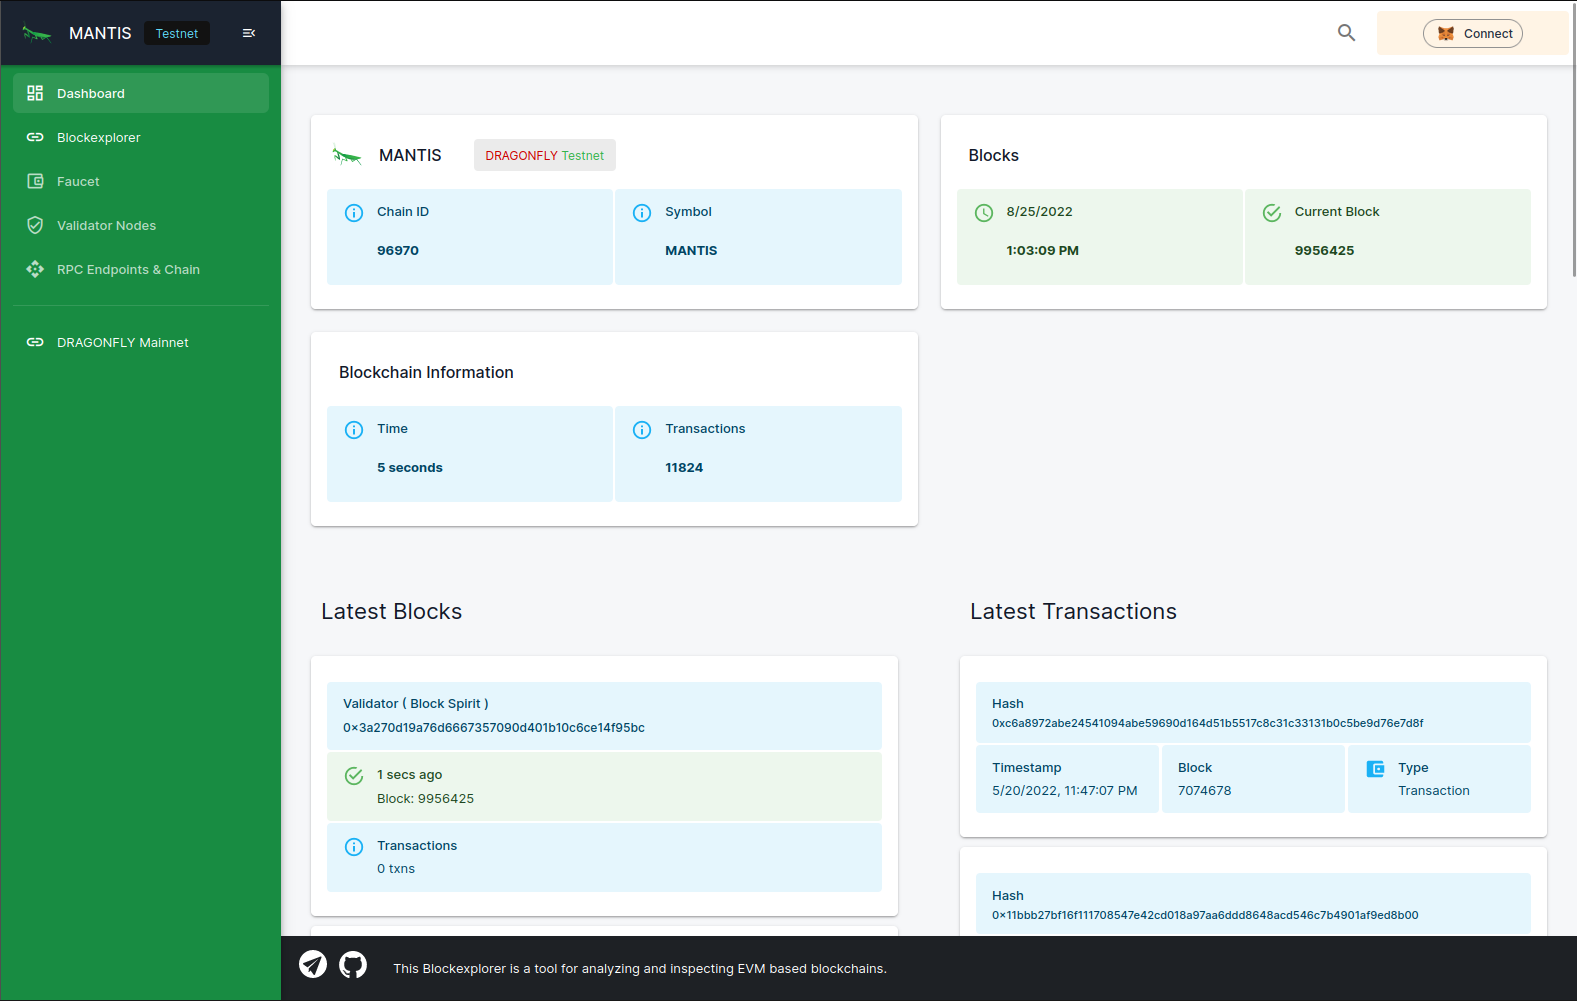
\includegraphics[width=\linewidth]{images/mantis_dashboard.png}%
  \caption{\label{fig:mantis_dashboard}Screenshot of the dashboard of the Mantis testnet.}
\end{figure}

\section{Screenshots}

Below are a few screenshots of the GitDAO demo application.

The homepage is shown in figure \cref{fig:demo_homepage}.
It displays the token that a user owns, the power left in each token as well as the proposal that the user can vote on.

\begin{figure}[ht!]
  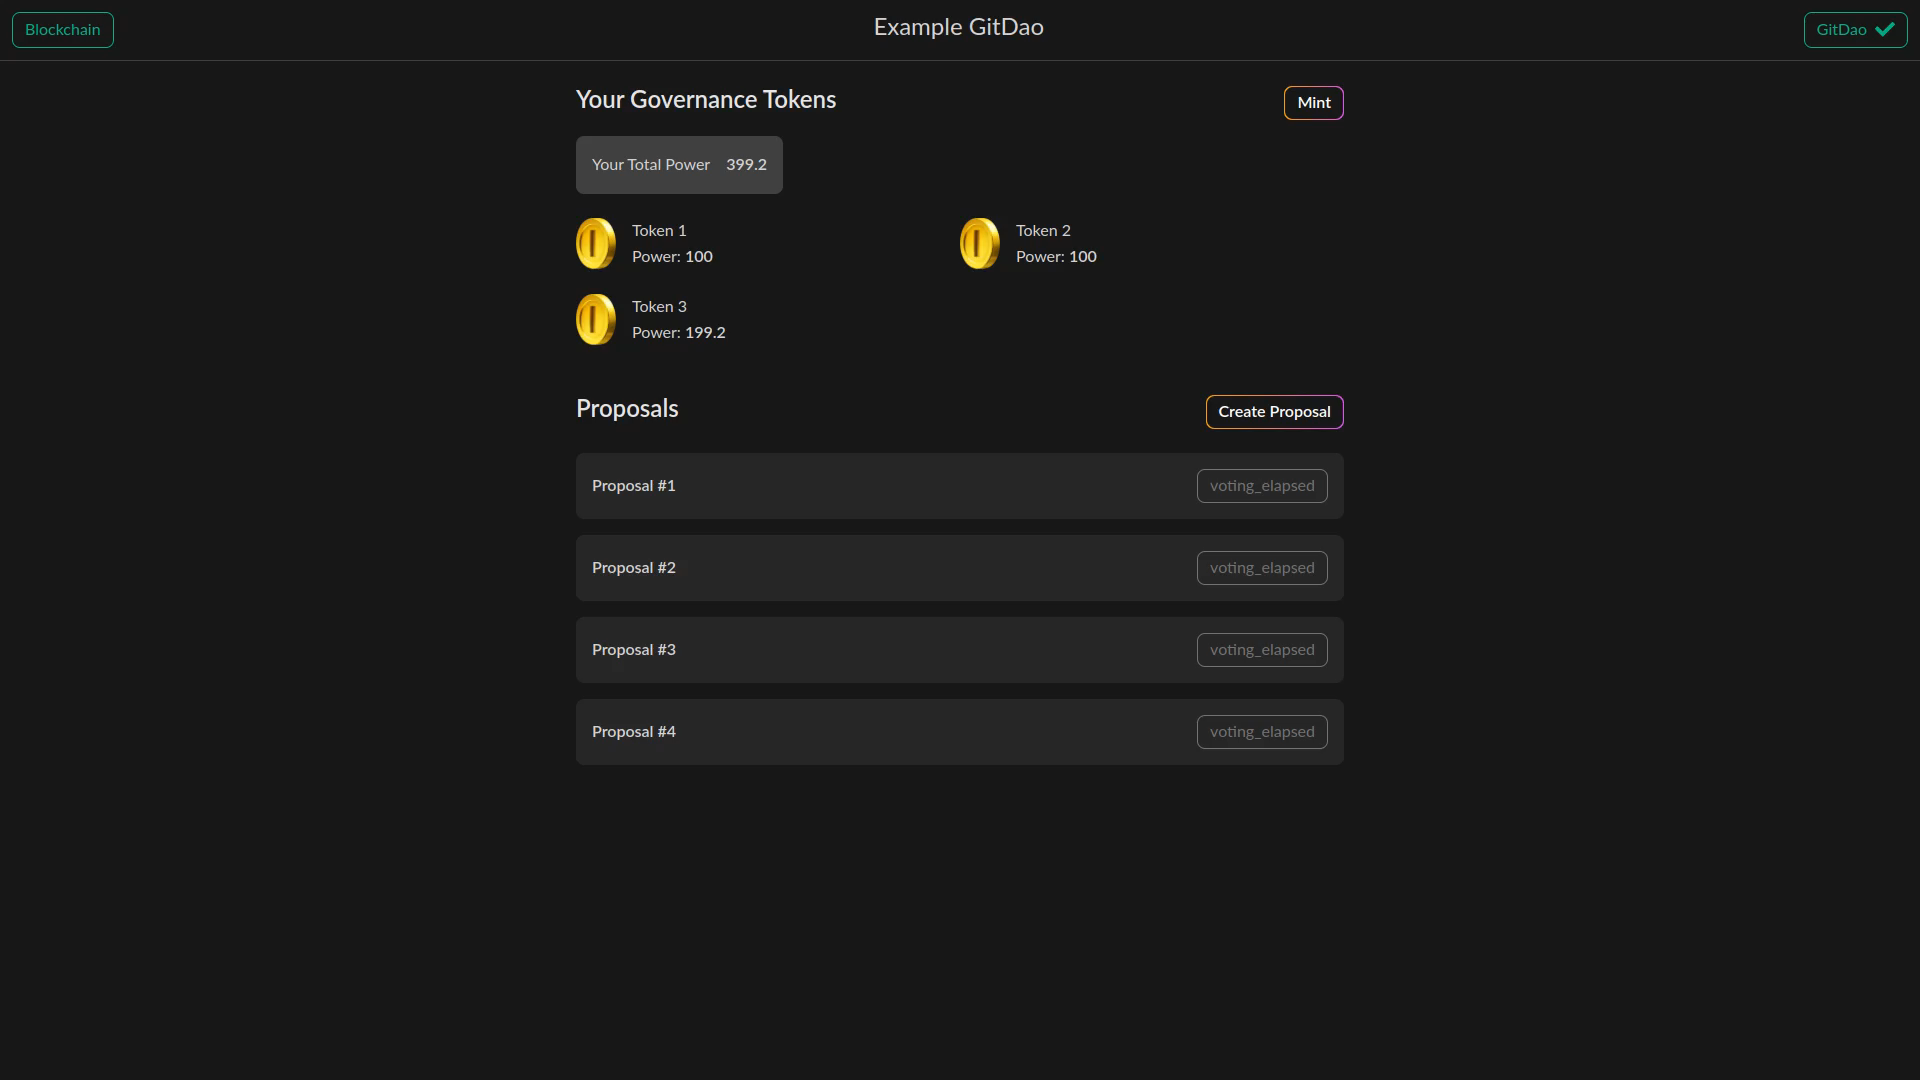
\includegraphics[width=\linewidth]{images/demo/homepage.png}
  \caption{\label{fig:demo_homepage}The homepage of the GitDAO demo.}
\end{figure}

The user can create a proposal, as shown in \cref{fig:demo_proposal_create}.
Once a proposal is created, the user can view it.
At first it will be in the \texttt{Pending} state (see \cref{fig:demo_proposal_read}).
Once the proposal enters the \texttt{Voting Opened} state (shown in \cref{fig:demo_proposal_opened}), the user will be able to vote on the proposal (see \cref{fig:demo_proposal_vote}) and the votes are shown on the proposal page as well (\cref{fig:demo_proposal_voted}).

\begin{figure}[ht!]
  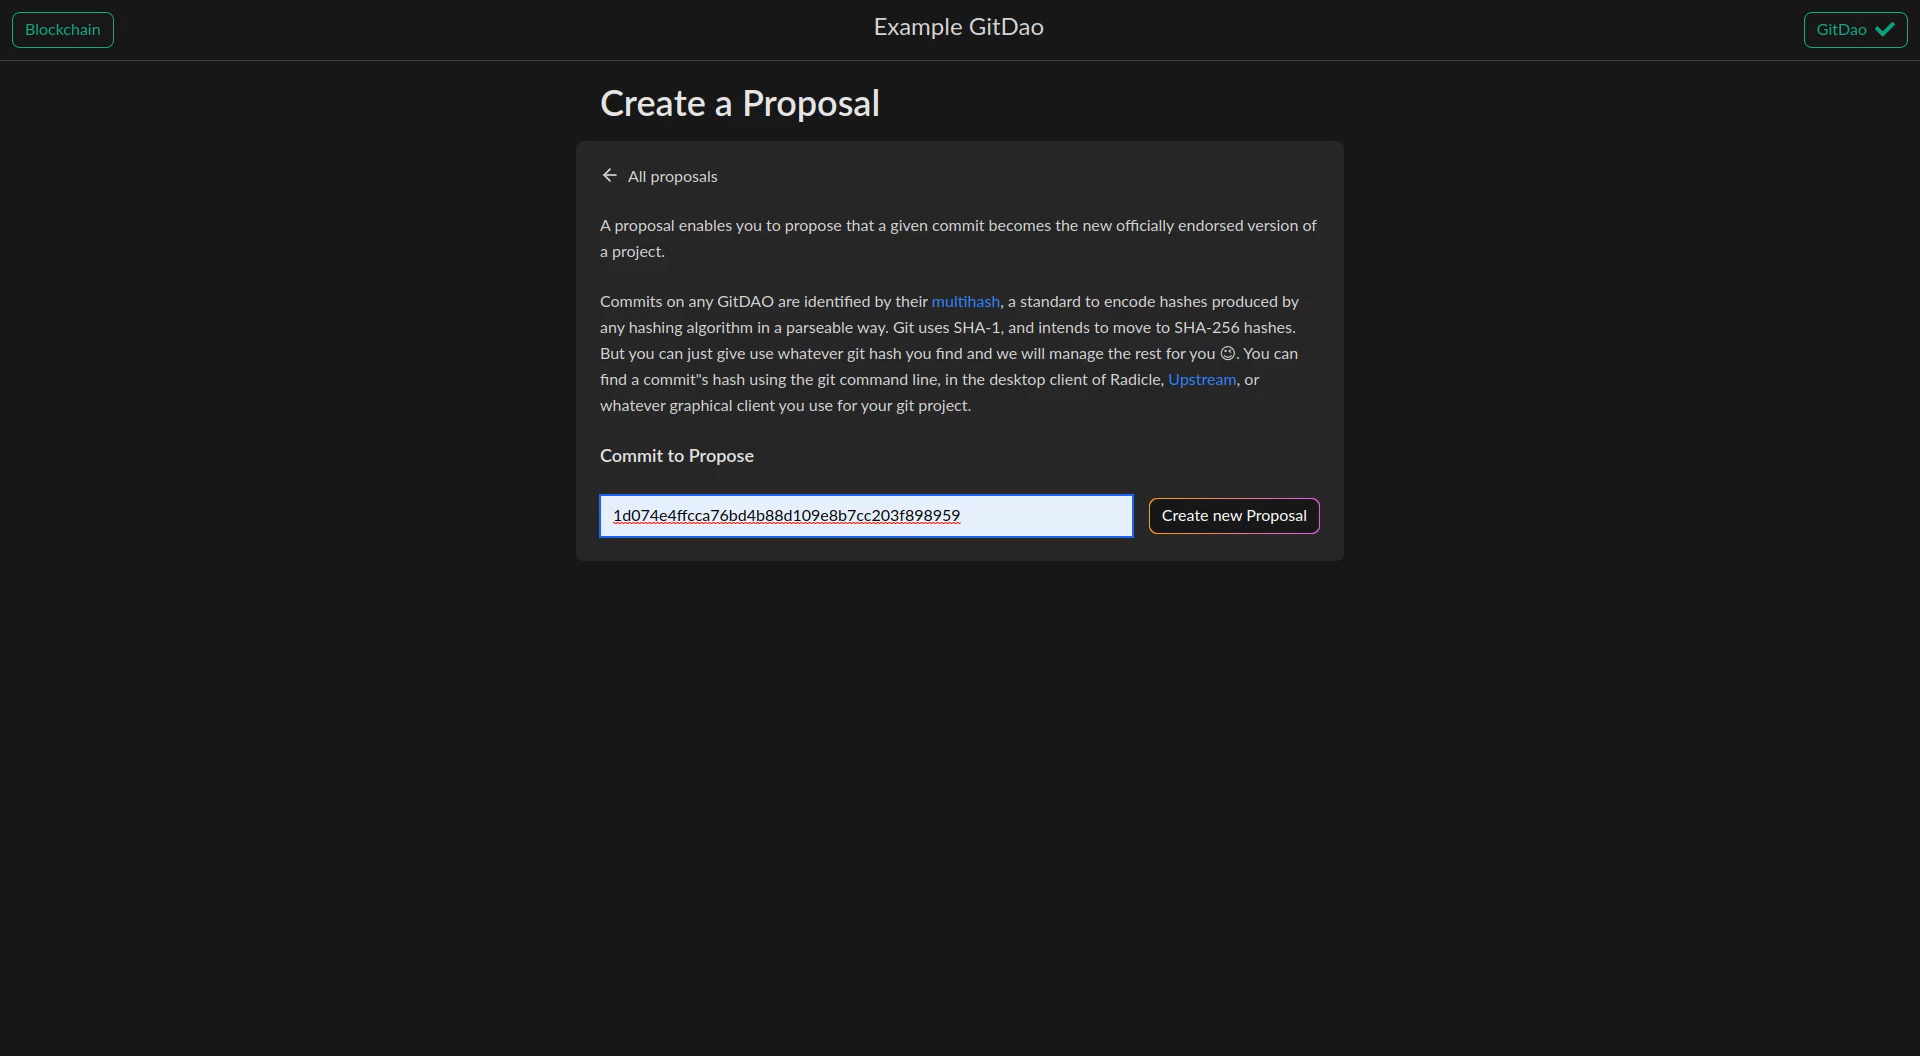
\includegraphics[width=\linewidth]{images/demo/proposal_create.png}
  \caption{\label{fig:demo_proposal_create}The proposal creation screen of the GitDAO demo.}
\end{figure}

\begin{figure}[ht!]
  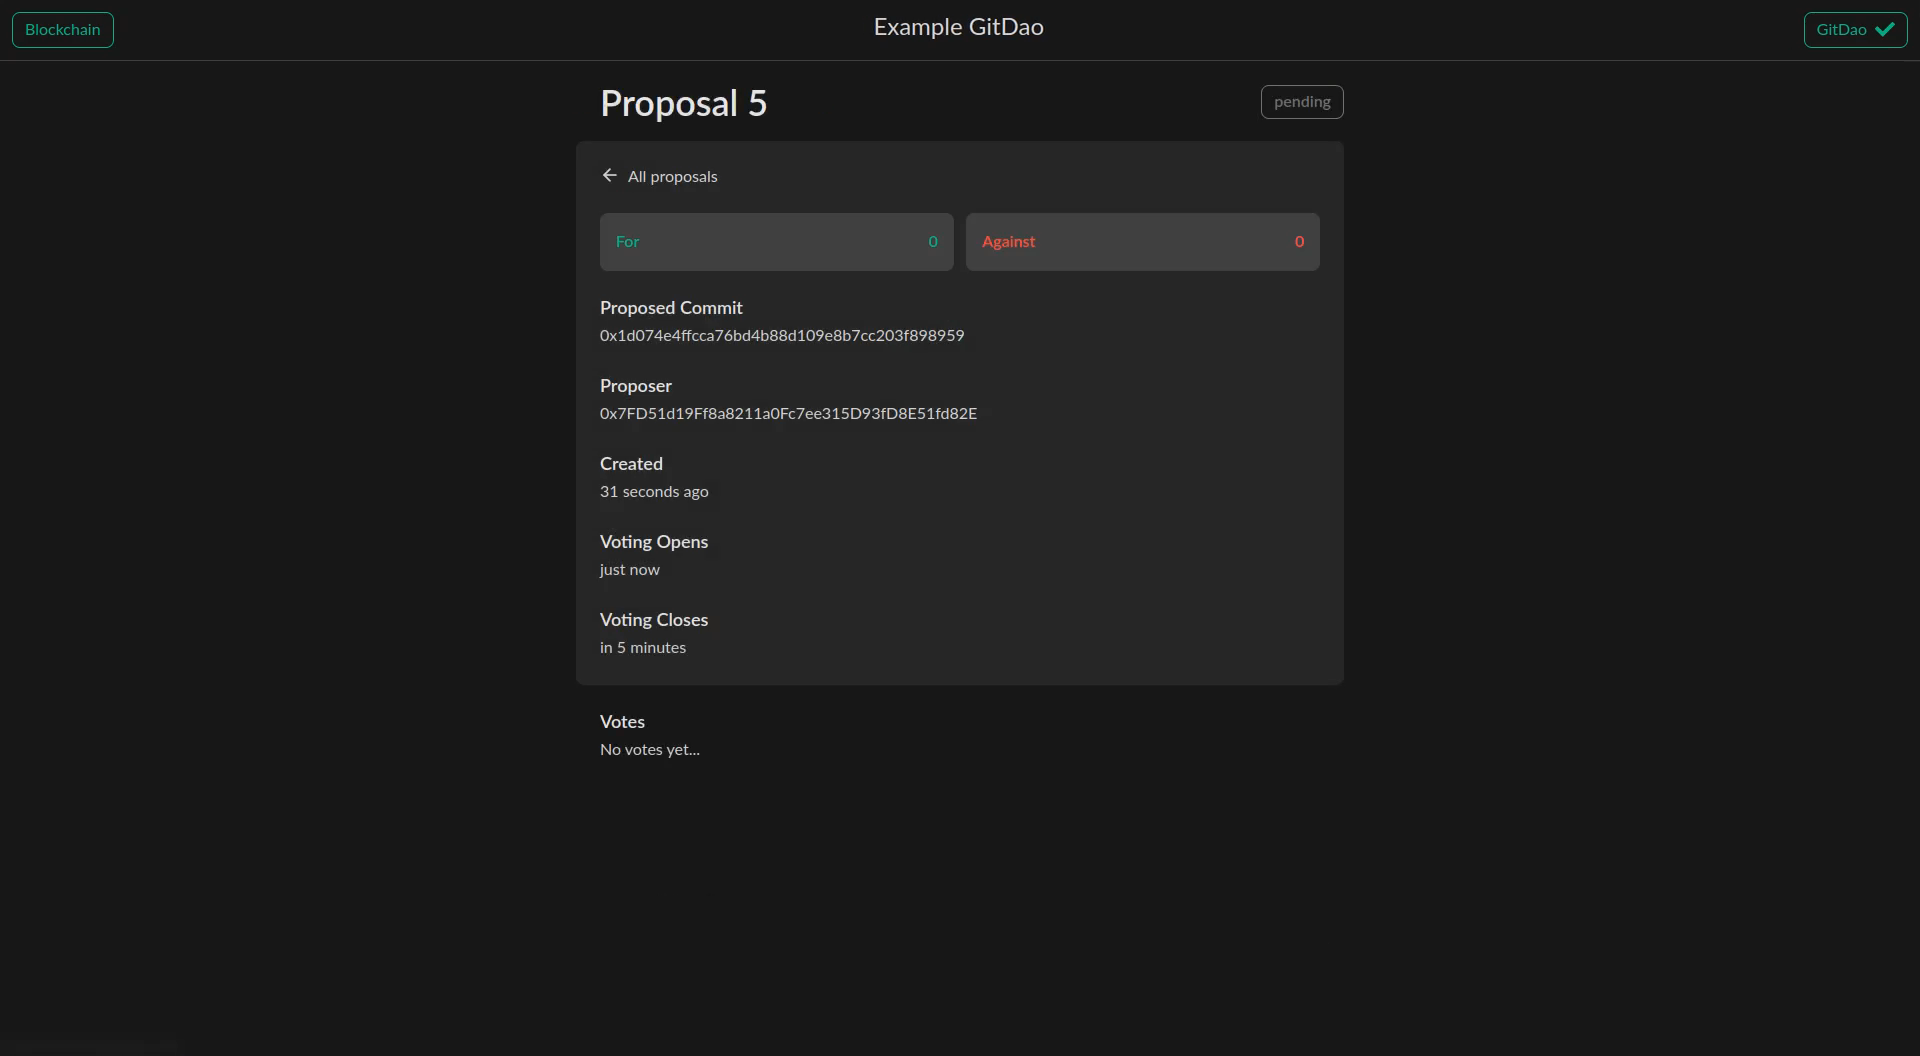
\includegraphics[width=\linewidth]{images/demo/proposal_read.png}
  \caption{\label{fig:demo_proposal_read}A proposal in pending state.}
\end{figure}

\begin{figure}[ht!]
  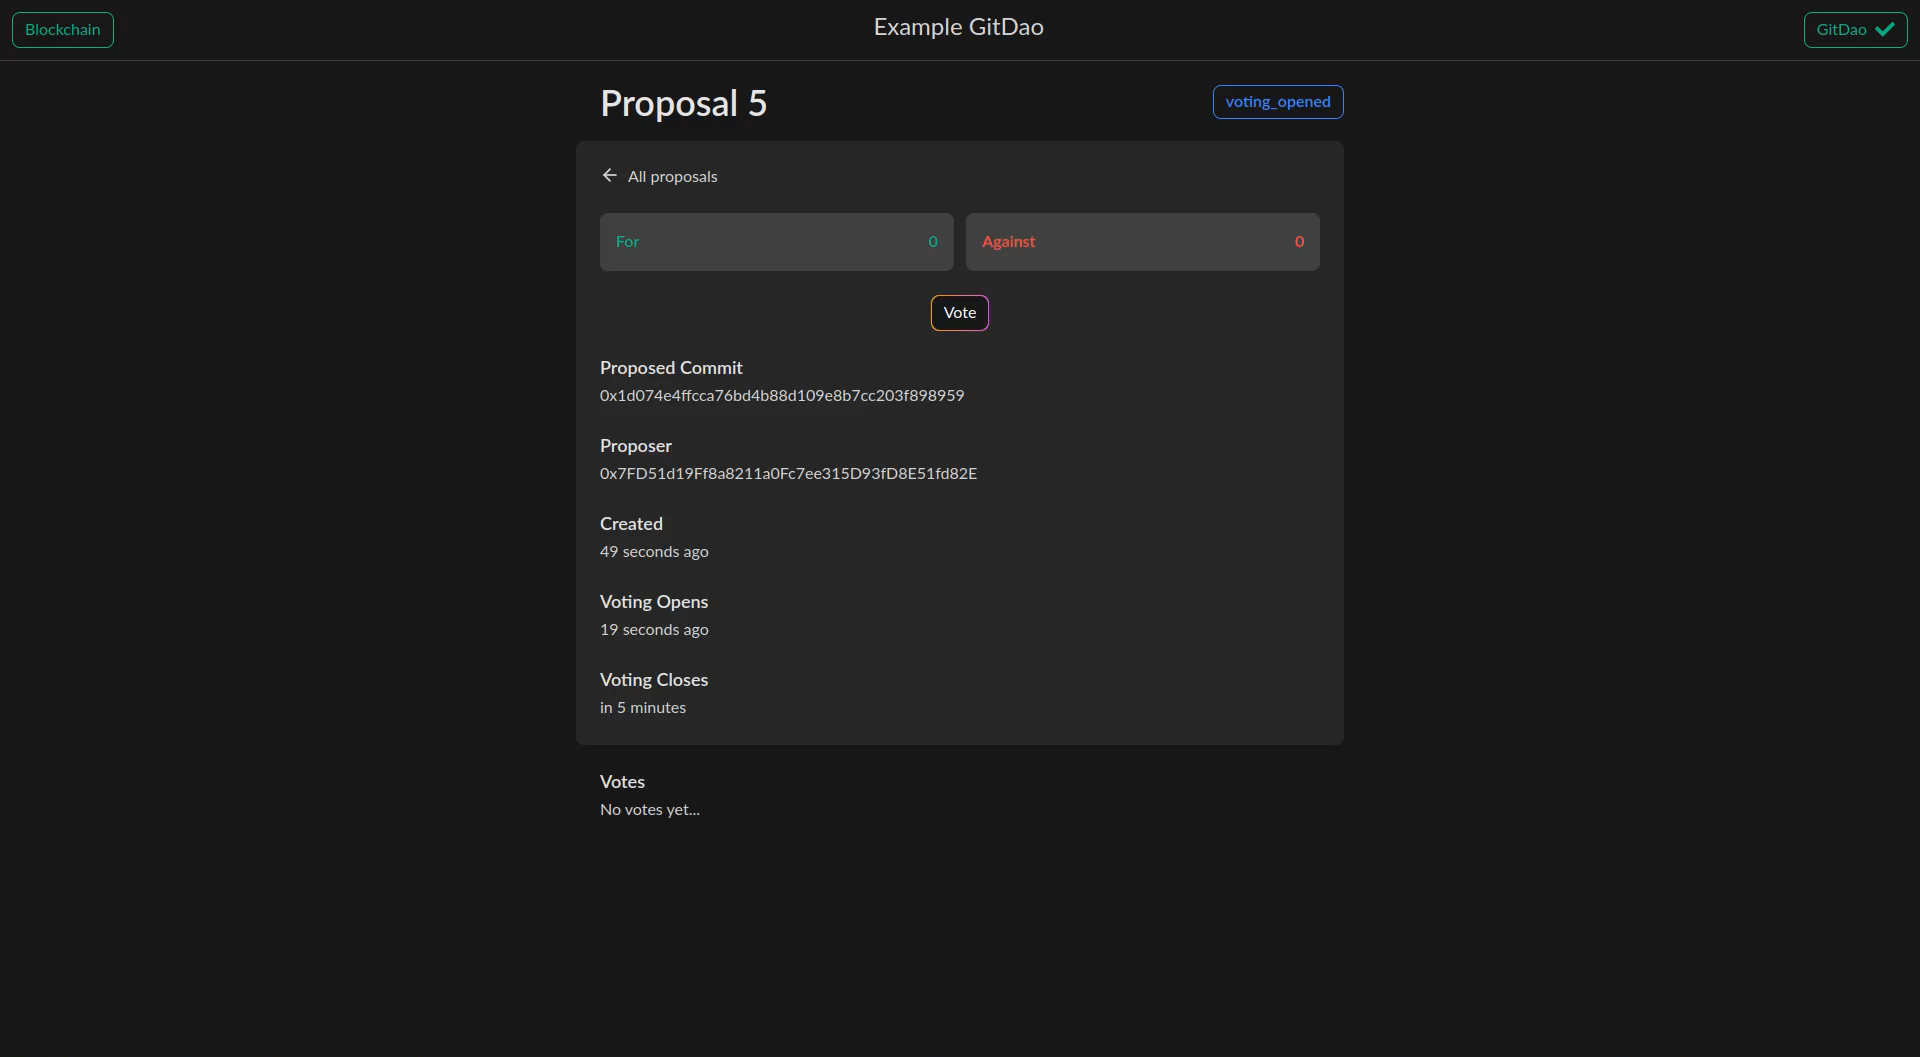
\includegraphics[width=\linewidth]{images/demo/proposal_read_opened.png}
  \caption{\label{fig:demo_proposal_opened}A proposal with voting opened.}
\end{figure}

\begin{figure}[ht!]
  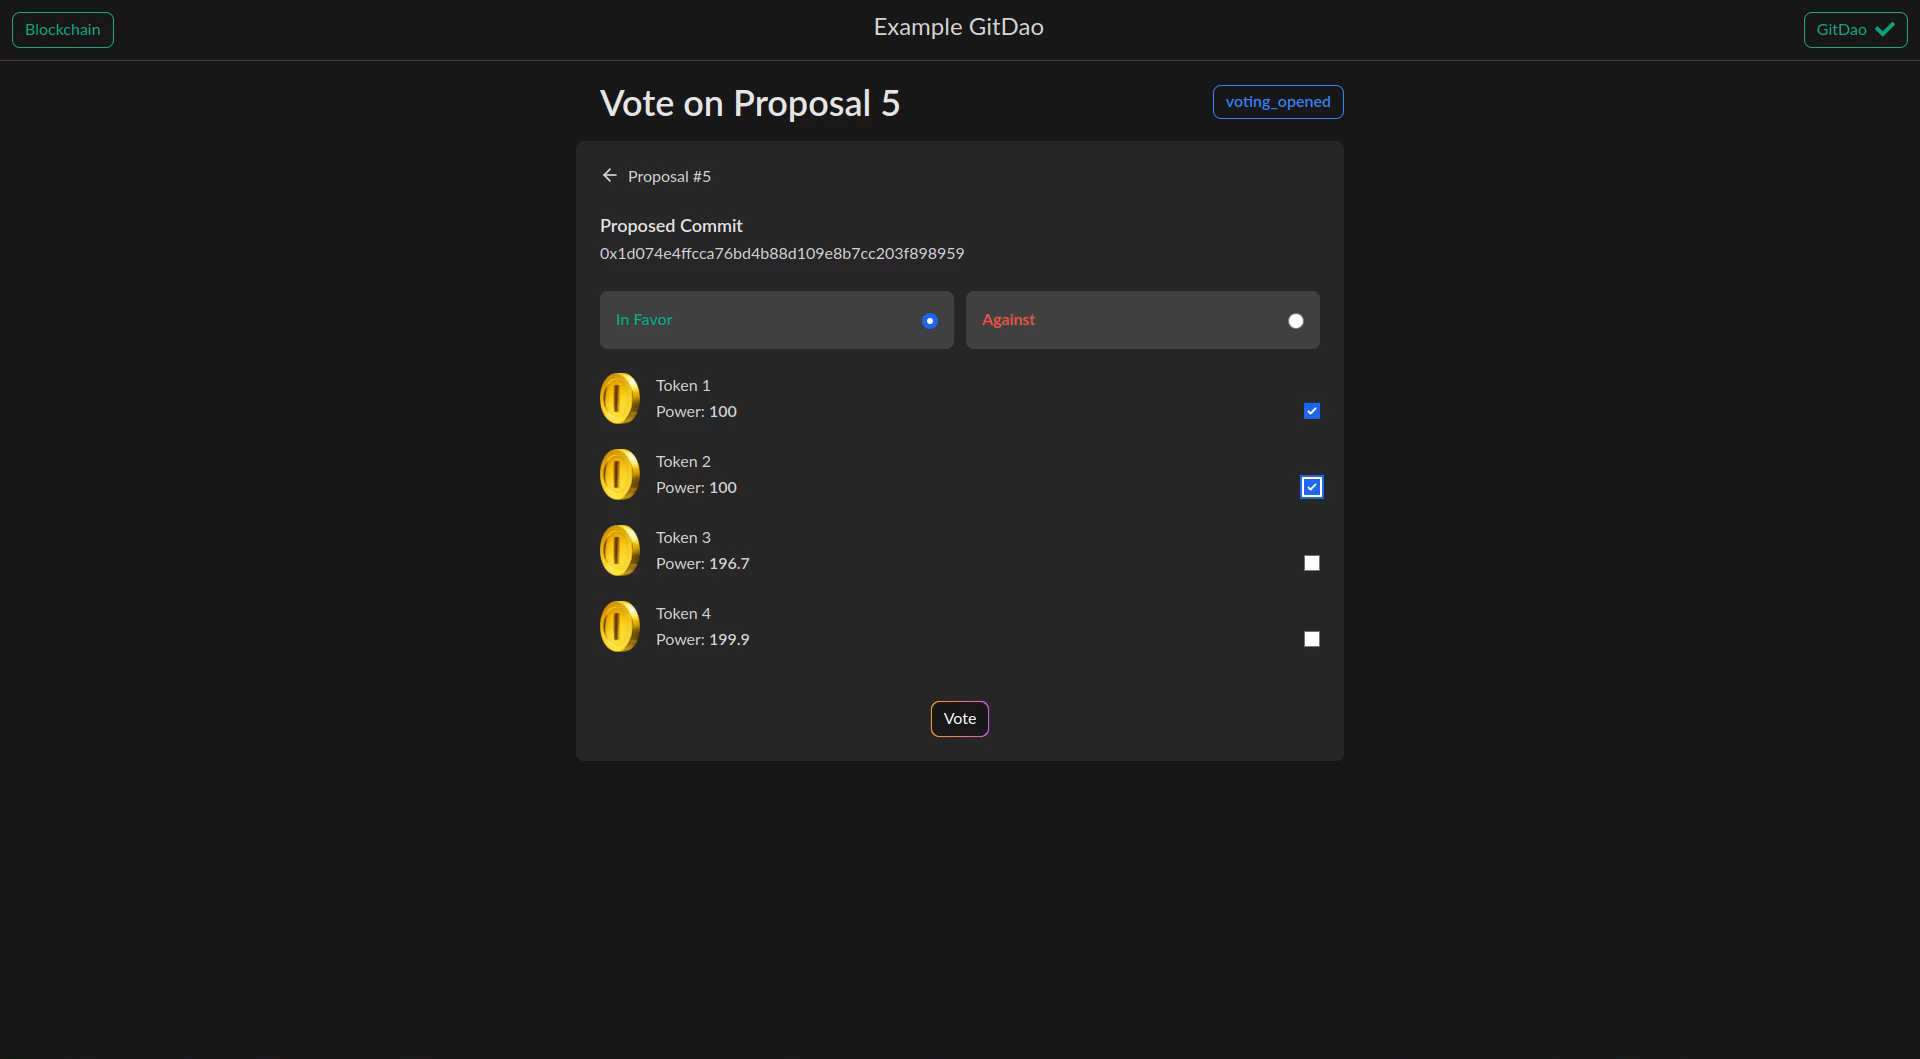
\includegraphics[width=\linewidth]{images/demo/proposal_vote.png}
  \caption{\label{fig:demo_proposal_vote}Voting screen.}
\end{figure}

\begin{figure}[ht!]
  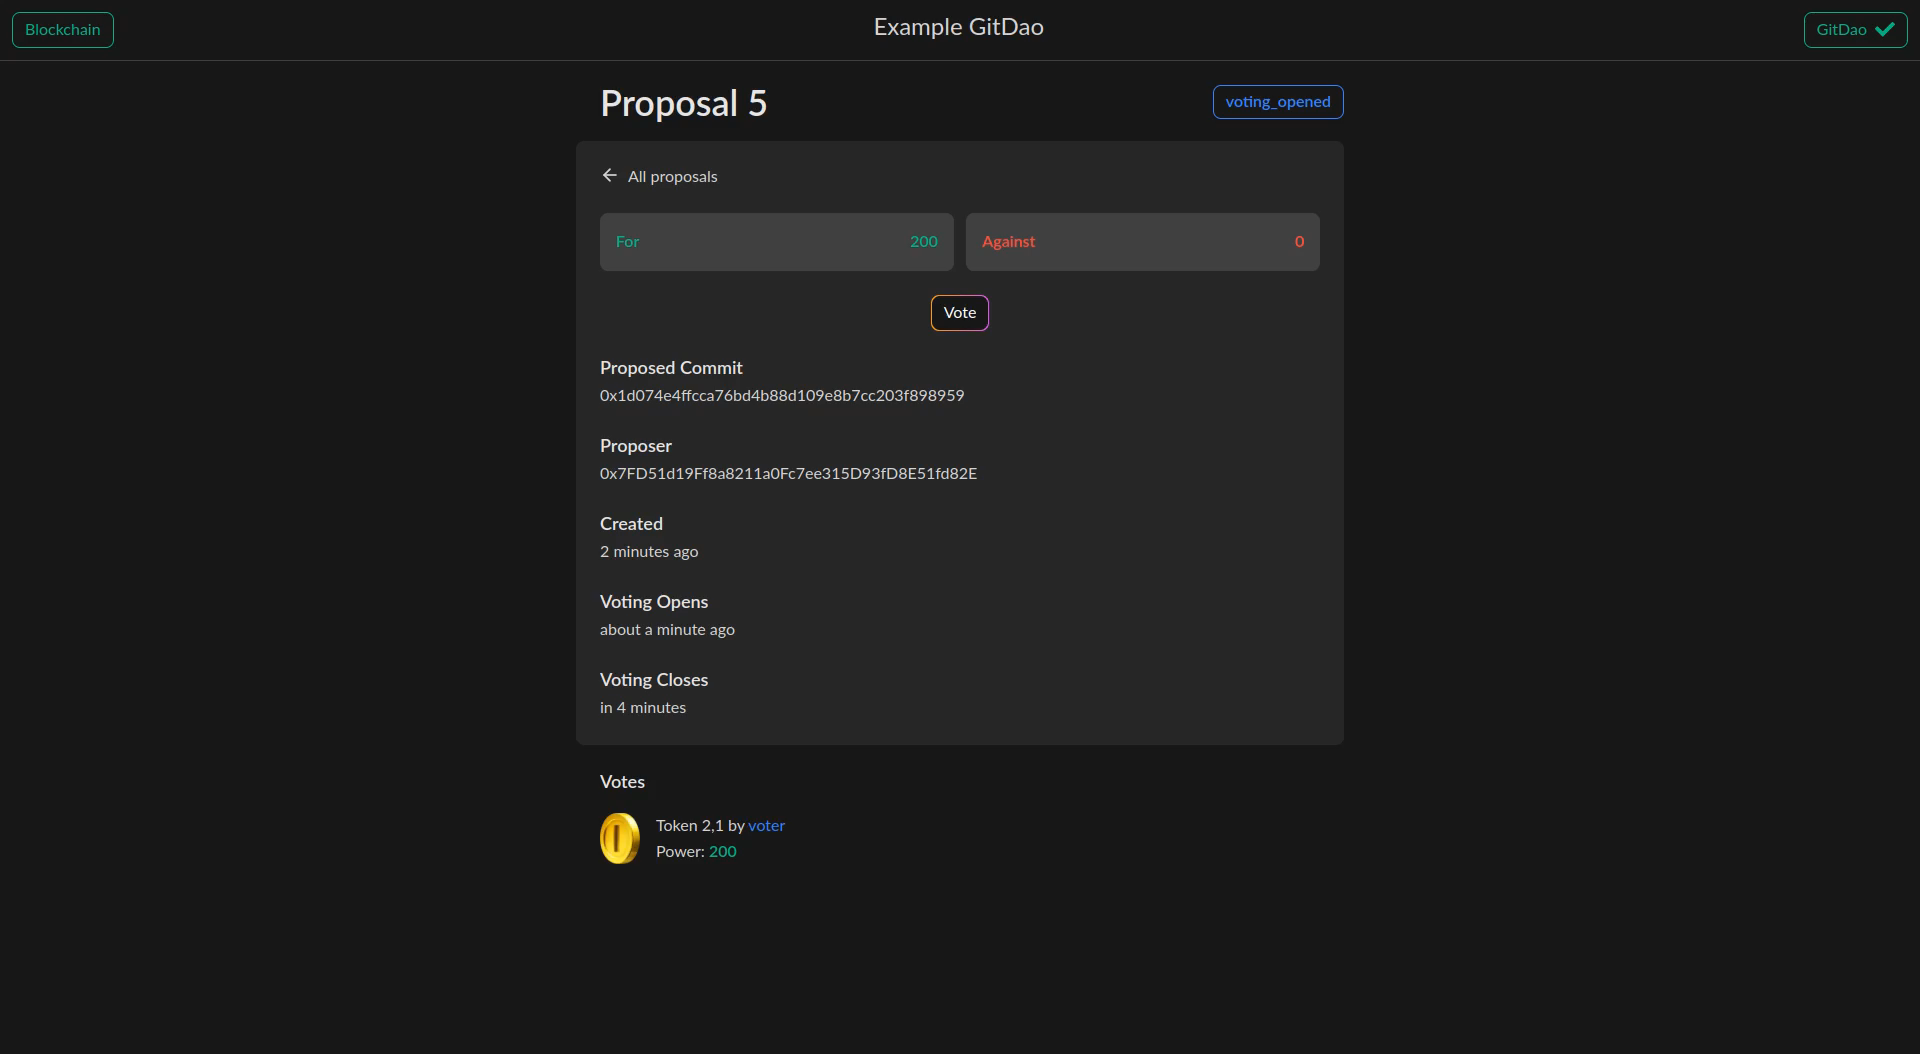
\includegraphics[width=\linewidth]{images/demo/proposal_read_voted.png}
  \caption{\label{fig:demo_proposal_voted}A proposal that received some votes.}
\end{figure}

\section{Development Details}

\marginElement{\centering
\includegraphics[width=.7\linewidth]{images/nix.png}}%
All the git repositories in this project are managed with nix\marginNote{See \href{https://nixos.org/}{nixos.org}.}, a functional package manager.
Nix, besides providing packages, provides a fully reproducible work environment called a nix \enquote{flake} as well as other goodies like command aliases.
This is a powerful tool that provides the guarantee that anyone is able to generate the same outputs in the future.
Through nix flakes it is possible to performs development operations like uploading a website to \textsc{ipfs} and pining this content on Pinata.

The backend code, i.e.\ the GitDAO smart contract is stored in a git repository stored at \url{https://gitlab.com/gitdao/gitdao}.
\marginElement{
  \tikz
    \node[fill=gray_10, inner sep=2mm, text width=\linewidth-4mm]{%
      \includesvg[width=\linewidth]{images/hardhat.svg}
    };
}%
We used hardhat as our Ethereum development environment; it provided us an Ethereum compiler, test frameworks, and tools to deploy to a blockchain of our choosing (like Mantis).

The frontend is a subroute of a blog deployed for this master thesis.
For \textsc{ud}-compatible browsers, use \url{the-git-dao.crypto/app.html}, otherwise the demo is deployed as a Heroku app: \url{https://the-git-dao.herokuapp.com/app}.
The code can be found at \url{https://gitlab.com/gitdao/website}.


\chapter{Radicle}
\label{sec:radicle}

This chapter is a chronology of our interactions with Radicle during this project.

\section{Discovering Radicle}

The original idea of this master thesis was to try to create some form of blockchain-based alternative to git.
This would allow easy integration between git and transfers of value.
One could imagine a system in which the creators of a piece of code get remunerated automatically when the code they wrote is executed.
This would create a business model for open source.
Of course, such a fundamental change in how code works is hard to bring about.

\marginElement{\centering\includesvg[width=.5\linewidth]{images/radicle.svg}}%
During some initial exploration of existing solutions, we were reminded of the existence of Radicle\marginNote{See \url{radicle.xyz}.}.
Radicle aims to provide \enquote{the decentralized code collaboration stack}, i.e.\ a peer-to-peer alternative to GitHub.

It seems helpful to remind the reader here of what features are part of git and what features are brought by overlays like GitHub, GitLab, Gitea, and consorts.
Git brings commits, commit trees and merge strategies (merge or rebase).
Overlays bring merge requests, tags, \textsc{ci/cd}, issues, and more.
Most of the social functionalities that we enjoy when coding comes from overlays.

Radicle's goal is to provide the same functionalities in a decentralized way.
Note that Radicle does not use any blockchain for that.
They designed their protocols based on gossiping, and while it does use some advanced cryptography, there is no economical or game theoretical framework like that of a blockchain.
Alleviating the need for a central entity is a difficult task, and so far Radicle has built \enquote{patches}, i.e.\ an alternative to merge requests, but it does not feature any social functionalities like comments or \textsc{ci/cd} (those are features planned for the future).

When we stumbled across the Radicle website, it became clear that it would be easier to integrate with Radicle than to build something similar ourselves.
Also, blockchains are not fundamentally adapted to hosting lots of data\marginNote{Storing $1$KB of data on Ethereum costs approximately 31\$ as of August 2022, which is prohibitively expensive.}, so building git on a blockchain is probably not the way to go (at least not as of 2022).

\section{Build a Radicle Org}

In March 2022, Radicle was featuring a new concept; \enquote{Orgs}.
Orgs were part of the blockchain integration featured at the time by the \textsc{gui} of Radicle called Upstream.
Orgs were a smart contract on Ethereum whose goal was to act as a registry of the \enquote{official} version of a project.
When the code becomes decentralized, potentially each developer of a single project has a different view of the code, in which different branches were merged and in a different order than the others.
So which version should be used by users of the project?
What is the official version?
To solve this issue, Radicle had Orgs.
But who controls an Org?
Who can decide what the official version of a project is?

Orgs could be any smart contract as long as the contract created \enquote{anchors}, where an anchor was the specification of how official commits had to be encoded.
This enabled great flexibility, as anyone could code its own Org and its decision system.
Radicle provided two Orgs templates.
One was an Org entirely controlled by a single individual, the other was based on a Gnosis safe, i.e.\ $m$ out of $n$ permissioned users of the Org had to agree to a proposed change.

Our initial idea was therefore to build an alternative Org for Radicle.
One that would be more akin to a DAO with a voting system based on a token (with decreasing value tokens and a way to handle donations).
So we settled for this task and built the demo and its underlying smart contract using the anchor interface from Radicle.

\section{Rug Pulled}

Once the demo was more or less completed, around the beginning of May, we tried to integrate our solution with Radicle.
We updated our Upstream version (to be sure to integrate with the latest and most up-to-date version) and soon discovered that all the blockchain integrations were removed from Upstream.

Some exploration of the Radicle forums led us to understand that Radicle was not dropping the idea of integrating with the blockchain, they only wanted to think it through and maybe propose additional features.

At this point, it is probably useful to give some additional details on how Radicle work.
The contributors of Radicle are split across \enquote{core teams}.
Each core team is responsible for one product of the Radicle ecosystem.
For example, there is a core team that builds the underlying peer-to-peer protocol of Radicle, another responsible for the Upstream client, another for the web and terminal interfaces, another that concerns itself with governance inside Radicle and interfacing with the Radicle foundation%
\marginNote{%
  The Radicle foundation gives a legal entity to the project.
  It is a Swiss foundation and it owns much of the large Radicle treasury.
}, yet another that builds Drips, a streamed payment protocol on the blockchain.
And, while some teams, like the Upstream team and the web and terminal interfaces team, favor some integration with the blockchain, this feeling does not appear to be shared by all: the protocol team remains rather skeptical of integrating with some blockchain.
Nevertheless, the situation this created was not particularly practical for the Master thesis you are reading.

We decided to reach out to Radicle and see whether it was possible to take part in the blockchain integration effort directly as a substitute for building an Org.

\section{Collaboration on Blockchain Integration}

The first problem was to find some individual that knew what was going on with the blockchain integration.
The only response we got from the Upstream team was that blockchain was paused for the time being.
By asking a bunch of people, we ended up talking with \#cloudhead, the person in charge of the \enquote{Alt. Clients} team (Alt. Clients means \enquote{alternative clients}, i.e.\ the web and terminal interfaces).
He seemed interested and we had a phone call.
He offered to compensate us for working on blockchain integration%
\marginNote{%
  We had to decline this offer because of \textsc{ethz} regulations.
}.
We did some brainstorming on the various possibilities that integrating Radicle with the blockchain offered.
The results of this brainstorming took the form of a Figma chart that is included in \cref{sec:figma}.

\section{EthCC}

Soon after that, so around the middle of July 2022, a major blockchain conference was happening in Paris.
Radicle was holding what they called an off-site, so many core members of the project met and we managed to meet a few%
\marginNote{%
  It is often surprising to confront the vision of someone you only know from chatting online and maybe having a phone call once with the actual physical person.
}.
While it was an interesting experience, it did not feel too inclusive.

\section{Stalemate}

After the EthCC break, work resumed on the blockchain integration.
We wrote a proposal for Radicle containing the principles described in this document.
The answer we got from \#cloudhead was strange to our ears...
He was proposing that the people that Radicle calls \enquote{delegate}%
\marginNote{%
  \textit{Delegates} of a Radicle repository, are originally constituted of only the account that creates a repository.
  This account can then add other delegates by granting them the delegate role.
} would have the voting power, and they could elect people that would get some payouts.
This sounded like a permissioned approach: it enshrines in the marble who has control over a project in a way that does not foster the inclusion of new contributors.

Another criticism addressed to our proposition was that it was never tried, there was no example of such a strategy working in practice.
This was also somewhat strange.
Radicle is creating new concepts regarding code collaborations (like that of a patch that does not work the same way as a merge request on GitHub), and new ways to interact.
That is the very concept of innovation, this is also the reason why so many people in the blockchain ecosystem are motivated by Radicle: it changes the status quo, it brings new ideas, and a new way to do things which is hopefully better than the previous one.
Why was it not welcome to innovate on governance models for open source projects?
Additionally, there are DAOs out there that do work in a fashion similar to GitDAO, for example, the Optimism DAO.

It was also raised that the proposed solution was too complex and did not solve an existing problem.
Preventing communities from forking because of a maintainer making decisions that are not consensual, through a token-based voting system, is valuable.
Providing a model to pay open source contributors also solves a real-life problem, namely, it improves incentives to contribute to open source and thus increases project longevity.
But at this point in the conversation, it wasn't clear anymore to us whether we were arguing rationally about the proposed solution, or if \#cloudhead had already made his made and was now trying to justify his opinion one way or another.
He might also have a biased opinion, as he is himself a delegate of many repositories hosted on Radicle.

After our last reply, we got no more responses.
As of the end of August, we sent a message to propose that we resume the conversation once the present work is completed.
Stalemate.

\section{A Personal Take on Radicle}

The history of Radicle helps to explain the current state of the project.
The project was co-founded in 2018 by Alexis Sellier (\#cloudhead) and Eleftherios Diakomichalis (\#lftherios).
The project has awakened a lot of interest from the blockchain ecosystem and raised around \$12M in 2021 \cite{noauthor_radicle_nodate}%
\marginNote{%
  As of August 2022, it was estimated that Radicle burns around \$500K per month \cite{noauthor_formal_nodate}.
}.
The Radicle Foundation which currently owns much of the treasury is governed by the two founders and Abbey Titcomb (\#abbey) \cite{noauthor_formal_nodate}.

\subsection{Too Much Money}

One issue that we see with the Radicle project is that a lot of time is spent on deciding how the money will be distributed and how governance will be conducted, and sometimes it feels like not much code is written.
It is our opinion that Radicle did not achieve much progress since March 2022.
In March, the Radicle website had more content, there was documentation, some Ethereum integration, and Radicle had a desktop client.
In August 2022, the website features less content, the desktop client has been sunsetted, the documentation is outdated (it explains how to interact with Radicle through the Upstream desktop client), and there is no more blockchain integration, but there are two new clients: one command line based, the other is a website.
In terms of features, Radicle is still too incomplete to become realistically usable.

Through the massive funding round that Radicle conducted in 2021, it received a lot of attention.
But by trying to become too big too early, a lot of time now has to be invested in coming up with governance systems, aligning the community, etc.
This is time that is not spent on actually building Radicle.
The initial vision was somewhat lost to the millions of dollars that the project received in investment.

\subsection{Lack of Consensual Vision}

As of August 2022, the community of Radicle is split into core teams, each team being intentionally very independent.
We think that this leads to some confusion, because the teams do not always want the same thing, and might decide to implement what they want without having a consensus from the others.
We guess that this is what happened with the Upstream client and the alternative clients (web and terminal).
In July 2022, Upstream was sunsetted, i.e.\ officially abandoned, and replaced by alternative clients.
Given that most of the functionalities required to make Radicle a viable alternative to GitHub are still missing (\textsc{ci/cd}, some mechanism to define the official version, blockchain integration, etc.), it might not be optimal to divide developer time on multiple clients and to sunset clients this early.
There seems to lack a common goal that everyone agrees on; the initial vision was somewhat blurry and now many people try to fill the holes in different ways.

Similarly, \#abbey wrote a blog post in February 2021 about Radicle releasing features that integrated with Ethereum.
Since then, the integration was removed and there are no clear plans for its future; neither about what it should entail nor about some release date.

\subsection{Hierarchy in Radicle}

Also, while the core teams might give the impression that they decentralize the control over the project, it feels to us that this creates some kind of hierarchy%
\marginElement{%
  \begin{center}
    Radicle Foundation\\
    $\downarrow$\\
    Core Team Owner (\#abbey, \#cloudhead and \#lftherios)\\
    $\downarrow$\\
    Core Team Member\\
    $\downarrow$\\
    Rest of the World
  \end{center}
} at the top of which stands the Radicle foundation.
Basically, and because decentralization is a core principle of Radicle, it was decided to separate the work in \enquote{core teams}.
Each of those teams is independent and focuses on a specific aspect of Radicle.
This approach has a few drawbacks; first, it silos information and vision for the project.
Second, it does not guarantee decentralization.
Indeed, each time is free to organize as it wishes, in reality, and as of August 2022, this means that each time has a benevolent dictator that leads the team; which is not decentralized.
Further, it enshrines a hierarchy in Radicle: team owners are the most influential individuals, then there are acknowledged team members, then the rest of the world.
And while such a model is standard in the corporate and startup worlds, this creates more barriers for new contributors than what is customary in the open source world%
\marginNote{%
  Even though similar structures exist in open source with the benevolent dictator of a project being the most powerful individual, followed by the \enquote{core} members, then the rest of the world which is often called \enquote{the halo}, the core members have no title that enshrines their status.
  Their influence appears organically as the sum of the interaction that those developers have with the project.
}.

Talks are being held to transfer the control of Radicle from the foundation to a DAO governed by the RAD token.
This is a step towards decentralization, except that the token distribution will change little to the current pretty centralized state of affairs...
As of August 2022, \#abbey owns 54\% of all RAD, and \#cloudhead has 24\% \cite{noauthor_sybil_nodate}...

\subsection{Lack of Alignment}

Finally, it seems strange that one of the founders of Radicle, \#cloudhead, would say that providing decentralized governance for code projects hosted on Radicle is not something that the project is interested in, even though the slogan of Radicle, until August 2022, was \enquote{Building the decentralized code collaboration stack}.
While it is not the same to build some decentralized infrastructure to host code and to build decentralized governance mechanisms to govern code (that might be hosted on a decentralized or centralized censorship-prone proprietary platform), both tasks have a lot in common, and experimenting on decentralized governance models ought to be an interest of the Radicle project.
Even more so since the Radicle project is trying to start a collaboration with Gitcoin, which aims at building public goods.
So while, we love the ideas underpinning the Radicle project, the interaction and the current state of affairs make us raise a few eyebrows.

\subsection{A Way Forward?}

As described in \cite{raymond_cathedral_2001}, successful projects need to provide a clear vision in the first place.
The Radicle project provided a slightly blurry vision, many details were initially left open.
While this impedes efficient work, this might not be a problem large enough to choke the project.

First, we believe that it is now important for Radicle to come up with a way to coordinate, to make the entire community agree on the way forward.
If the initial vision was not clear enough, then a way needs to be found to fill it out.

Second, the focus needs to switch from \enquote{how people will make money} to \enquote{how the project will be turned into working software that people use and love}.

Finally, the project needs to be more inclusive of contributors, no more changing the domain names of the website every month, clear and complete documentation to make it easy for people to contribute%
\marginNote{%
  The Radicle documentation, at times, was changed without providing any ways to view previous versions of it, for example, all Org documentation was removed when the blockchain integration was removed from Upstream.
  The documentation was completely removed with the August 2022 version of the main website.
  The Radicle blog, which contained various articles on the RAD token and the Radicle vision, was also deleted with the August 2022 version of the website.
}, and a more inclusive process to onboard people that want to contribute%
\marginNote{%
  Holding an invite-only meeting with all the members considered \enquote{core} enough during EthCC is not an inclusive way to make progress.
  This goes against the ideals of transparency and inclusion that are important to the open source movement, the blockchain movement, and Radicle's values.
}.



\nomargintoc
\nomarginimagecaption%
\chapter{Conclusion}
\label{sec:conclusion}

\leavevmode\marginElement{Open source represents critical infrastructure for today's societies, yet we fail to protect it accordingly.}%
\marginElement{\input{images/sectioning/horizontal/\arabic{image_sectioning_horizontal}/readme.tex}}%
It is a rather undisputed fact that the world runs on open source.
To give only one example, it is estimated that WordPress, an open source website framework, ran approximately 42\% of all the websites in October 2021 \cite{noauthor_wordpress_2022}.
Any software today, somewhere in its dependencies, uses a piece of open source code, if only because the very majority of the most used programming languages are open source.
Nevertheless, as a society, we do not yet act accordingly; we fail to acknowledge how critical the infrastructure that powers our societies is, and so we do not protect it enough.
\textcquote{filippo_valsorda_professional_2021}{The status quo is unmaintainable.}
We need a mentality shift, we need to inject more money into the open source, and we need to build incentive systems that provide us with more guarantees.

\leavevmode\marginElement{The goal of this work: improve open source \emph{trustlessness} by designing new, blockchain-based coordination systems.}%
This is what we call \emph{making open source trustless}: being able to trust open source to create only positive outputs, without having to trust any individual contributors.
If open source becomes trustless, then society is better off.
To improve the trustlessness of open source, we proposed in this work to focus on designing new coordination systems.
We used blockchain as the technological foundation because it is trustless itself.
Using any trustful technology instead would prevent us from achieving trustlessness.

\leavevmode\marginElement{Coordination systems are hard.}%
Unfortunately, designing good coordination systems is difficult.
This research field needs to combine math, game theory, psychology, philosophy, economics, and computer science.
There are a great variety of properties that we wish these systems to offer: security in the face of adversarial agents, Pareto efficiency, minimum friction, etc.
And we know that we cannot have it all: nature imposes some fundamental limitations, like Arrow's impossibility theorem; some properties conflict with one another, like privacy and transparency; and we must design those systems around human limitations, like the recency bias.

\leavevmode\marginElement{Decentralization is a key to trustlessness.}%
Bringing \emph{trustlessness} to open source, our ultimate goal, requires at least \emph{decentralization}; indeed, a system cannot be trustless if it is centralized.
We proposed that there are two key components to being decentralized.
First, there need to be many actors involved; second, each actor needs to have the same power as the others.
We also put forward, that building systems that naturally revert to a decentralized state, i.e.\ what we defined as \emph{progressive decentralization}, is an approach more resilient, than building a system that is decentralized to begin with, and hoping that it remains so afterward.
Especially knowing that power often acts as a reinforcement loop, i.e.\ having power enables getting more power.

\leavevmode\marginElement{Decentralization and open source.}%
Open source projects always begin in a centralized state anyways, because they are initiated by at most a few individuals.
So building initially decentralized systems is hopeless, and only progressive decentralization can bring decentralization about.
Through the core/halo categorization, it is understood that most open source projects today never managed to decentralize: the power is in the hands of a few core developers.
There is much that can be improved.

\leavevmode\marginElement{Importance of \textit{proof of personhood}.}%
In this work, we proposed that an intrinsic progressive decentralization system, so a system in which the power distribution reverts to the uniform distribution unless power differences are continuously maintained over time, through repeated, valuable contributions, can only be built, if a satisfying answer to \textit{proof of personhood} is found.

\leavevmode\marginElement{Proposed blockchain primitives.}%
While intrinsic progressive decentralization is currently not achievable, this work proposed primitives that improve various aspects of trustlessness:

\begin{description}
  \item[Decreasing Power Governance Tokens]
    provide incentives for newcomers to participate, and for members to contribute regularly.
    This improves the first aspect of decentralization: widening the community of a project and shrinking the gap between highly active and less active members, by incentivizing regular contributions.
    By distributing the power to all those that participate, the system is an improvement over the Benevolent Dicta\-tor for Life model that most open source projects use today.
  \item[The Voting Workflow]
    specifically suited to merge requests improves the security guarantees over the code accepted.
    The challenge mechanism further deters adversarial behaviors.
  \item[The Rewarding Scheme]
    to award tokens in compensation for the value provided to a project realigns value creation and value extraction.
    This creates incentives to provide more value.
  \item[The Money Distribution Process]
    rewards developers in a fair way.
    Paying developers can transform contributing to open source into a sustainable activity, thus it improves projects' longevity.
    We also discussed the possibility of using Radicle Drips to split part of the received money and donate it to the dependencies of a project.
    This creates a funding graph through the open source ecosystem, thus even the most hidden, but fundamental, open source libraries could receive money.
  \item[Issue Backing]
    provides a way for users to communicate preferences to developers, which makes it possible for open source projects to provide more value to society.
    It also increases the amount of money sent to open source projects and their developers.
\end{description}

\leavevmode\marginElement{Solving cooperation issues at large.}%
The 21\textsuperscript{st} century will be one of many challenges.
The human population is larger than ever, and problems scale accordingly.
Technological developments have made us more powerful than ever and the consequences of our actions scale accordingly.
This is why coordination failures today have more dramatic consequences: wars are more destructive, economical crises impact more humans.
Climate change is the embodiment of the impacts that failing to coordinate around a public good yield.
We need to improve our governance systems if we are to solve these issues.
We need governments and companies that are more representative, more transparent, more efficient, more aligned with humanity's shared goals, and more cooperative among themselves.
We hope that the primitives listed above contribute to making open source more \emph{trustless}.
We hope that they improve human coordination.


\part{Appendices}
% \partSecondPage%

\appendix

\nomargintoc\chapter{\textsc{Snafu} Fable}
\label{sec:snafu_fable}

In the beginning was the plan,\\
and then the specification;\\
And the plan was without form,\\
and the specification was void.

And darkness\\
was on the faces of the implementors thereof;\\
And they spake unto their leader,\\
saying:\\
"It is a crock of shit,\\
and smells as of a sewer."

And the leader took pity on them,\\
and spoke to the project leader:\\
"It is a crock of excrement,\\
and none may abide the odor thereof."

And the project leader\\
spake unto his section head, saying:\\
"It is a container of excrement,\\
and it is very strong, such that none may abide it."

The section head then hurried to his department manager,\\
and informed him thus:\\
"It is a vessel of fertilizer,\\
and none may abide its strength."

The department manager carried these words\\
to his general manager,\\
and spoke unto him\\
saying:\\
"It containeth that which aideth the growth of plants,\\
and it is very strong."

And so it was that the general manager rejoiced\\
and delivered the good news unto the Vice President.\\
"It promoteth growth,\\
and it is very powerful."

The Vice President rushed to the President's side,\\
and joyously exclaimed:\\
"This powerful new software product\\
will promote the growth of the company!"

And the President looked upon the product,\\
and saw that it was very good.

\cite{noauthor_snafu_nodate}



%\listofdefinitions
\printbibliography

\end{document}

